% Options for packages loaded elsewhere
\PassOptionsToPackage{unicode}{hyperref}
\PassOptionsToPackage{hyphens}{url}
%
\documentclass[
]{book}
\usepackage{lmodern}
\usepackage{amsmath}
\usepackage{ifxetex,ifluatex}
\ifnum 0\ifxetex 1\fi\ifluatex 1\fi=0 % if pdftex
  \usepackage[T1]{fontenc}
  \usepackage[utf8]{inputenc}
  \usepackage{textcomp} % provide euro and other symbols
  \usepackage{amssymb}
\else % if luatex or xetex
  \usepackage{unicode-math}
  \defaultfontfeatures{Scale=MatchLowercase}
  \defaultfontfeatures[\rmfamily]{Ligatures=TeX,Scale=1}
\fi
% Use upquote if available, for straight quotes in verbatim environments
\IfFileExists{upquote.sty}{\usepackage{upquote}}{}
\IfFileExists{microtype.sty}{% use microtype if available
  \usepackage[]{microtype}
  \UseMicrotypeSet[protrusion]{basicmath} % disable protrusion for tt fonts
}{}
\makeatletter
\@ifundefined{KOMAClassName}{% if non-KOMA class
  \IfFileExists{parskip.sty}{%
    \usepackage{parskip}
  }{% else
    \setlength{\parindent}{0pt}
    \setlength{\parskip}{6pt plus 2pt minus 1pt}}
}{% if KOMA class
  \KOMAoptions{parskip=half}}
\makeatother
\usepackage{xcolor}
\IfFileExists{xurl.sty}{\usepackage{xurl}}{} % add URL line breaks if available
\IfFileExists{bookmark.sty}{\usepackage{bookmark}}{\usepackage{hyperref}}
\hypersetup{
  pdftitle={Kursmaterial Introduktion till R - Certifierad Data Scientist},
  pdfauthor={Filip Wästberg \& Torbjörn Sjöberg, Solita},
  hidelinks,
  pdfcreator={LaTeX via pandoc}}
\urlstyle{same} % disable monospaced font for URLs
\usepackage{color}
\usepackage{fancyvrb}
\newcommand{\VerbBar}{|}
\newcommand{\VERB}{\Verb[commandchars=\\\{\}]}
\DefineVerbatimEnvironment{Highlighting}{Verbatim}{commandchars=\\\{\}}
% Add ',fontsize=\small' for more characters per line
\usepackage{framed}
\definecolor{shadecolor}{RGB}{248,248,248}
\newenvironment{Shaded}{\begin{snugshade}}{\end{snugshade}}
\newcommand{\AlertTok}[1]{\textcolor[rgb]{0.94,0.16,0.16}{#1}}
\newcommand{\AnnotationTok}[1]{\textcolor[rgb]{0.56,0.35,0.01}{\textbf{\textit{#1}}}}
\newcommand{\AttributeTok}[1]{\textcolor[rgb]{0.77,0.63,0.00}{#1}}
\newcommand{\BaseNTok}[1]{\textcolor[rgb]{0.00,0.00,0.81}{#1}}
\newcommand{\BuiltInTok}[1]{#1}
\newcommand{\CharTok}[1]{\textcolor[rgb]{0.31,0.60,0.02}{#1}}
\newcommand{\CommentTok}[1]{\textcolor[rgb]{0.56,0.35,0.01}{\textit{#1}}}
\newcommand{\CommentVarTok}[1]{\textcolor[rgb]{0.56,0.35,0.01}{\textbf{\textit{#1}}}}
\newcommand{\ConstantTok}[1]{\textcolor[rgb]{0.00,0.00,0.00}{#1}}
\newcommand{\ControlFlowTok}[1]{\textcolor[rgb]{0.13,0.29,0.53}{\textbf{#1}}}
\newcommand{\DataTypeTok}[1]{\textcolor[rgb]{0.13,0.29,0.53}{#1}}
\newcommand{\DecValTok}[1]{\textcolor[rgb]{0.00,0.00,0.81}{#1}}
\newcommand{\DocumentationTok}[1]{\textcolor[rgb]{0.56,0.35,0.01}{\textbf{\textit{#1}}}}
\newcommand{\ErrorTok}[1]{\textcolor[rgb]{0.64,0.00,0.00}{\textbf{#1}}}
\newcommand{\ExtensionTok}[1]{#1}
\newcommand{\FloatTok}[1]{\textcolor[rgb]{0.00,0.00,0.81}{#1}}
\newcommand{\FunctionTok}[1]{\textcolor[rgb]{0.00,0.00,0.00}{#1}}
\newcommand{\ImportTok}[1]{#1}
\newcommand{\InformationTok}[1]{\textcolor[rgb]{0.56,0.35,0.01}{\textbf{\textit{#1}}}}
\newcommand{\KeywordTok}[1]{\textcolor[rgb]{0.13,0.29,0.53}{\textbf{#1}}}
\newcommand{\NormalTok}[1]{#1}
\newcommand{\OperatorTok}[1]{\textcolor[rgb]{0.81,0.36,0.00}{\textbf{#1}}}
\newcommand{\OtherTok}[1]{\textcolor[rgb]{0.56,0.35,0.01}{#1}}
\newcommand{\PreprocessorTok}[1]{\textcolor[rgb]{0.56,0.35,0.01}{\textit{#1}}}
\newcommand{\RegionMarkerTok}[1]{#1}
\newcommand{\SpecialCharTok}[1]{\textcolor[rgb]{0.00,0.00,0.00}{#1}}
\newcommand{\SpecialStringTok}[1]{\textcolor[rgb]{0.31,0.60,0.02}{#1}}
\newcommand{\StringTok}[1]{\textcolor[rgb]{0.31,0.60,0.02}{#1}}
\newcommand{\VariableTok}[1]{\textcolor[rgb]{0.00,0.00,0.00}{#1}}
\newcommand{\VerbatimStringTok}[1]{\textcolor[rgb]{0.31,0.60,0.02}{#1}}
\newcommand{\WarningTok}[1]{\textcolor[rgb]{0.56,0.35,0.01}{\textbf{\textit{#1}}}}
\usepackage{longtable,booktabs}
\usepackage{calc} % for calculating minipage widths
% Correct order of tables after \paragraph or \subparagraph
\usepackage{etoolbox}
\makeatletter
\patchcmd\longtable{\par}{\if@noskipsec\mbox{}\fi\par}{}{}
\makeatother
% Allow footnotes in longtable head/foot
\IfFileExists{footnotehyper.sty}{\usepackage{footnotehyper}}{\usepackage{footnote}}
\makesavenoteenv{longtable}
\usepackage{graphicx}
\makeatletter
\def\maxwidth{\ifdim\Gin@nat@width>\linewidth\linewidth\else\Gin@nat@width\fi}
\def\maxheight{\ifdim\Gin@nat@height>\textheight\textheight\else\Gin@nat@height\fi}
\makeatother
% Scale images if necessary, so that they will not overflow the page
% margins by default, and it is still possible to overwrite the defaults
% using explicit options in \includegraphics[width, height, ...]{}
\setkeys{Gin}{width=\maxwidth,height=\maxheight,keepaspectratio}
% Set default figure placement to htbp
\makeatletter
\def\fps@figure{htbp}
\makeatother
\setlength{\emergencystretch}{3em} % prevent overfull lines
\providecommand{\tightlist}{%
  \setlength{\itemsep}{0pt}\setlength{\parskip}{0pt}}
\setcounter{secnumdepth}{5}
\usepackage{booktabs}
\ifluatex
  \usepackage{selnolig}  % disable illegal ligatures
\fi

\title{Kursmaterial Introduktion till R - Certifierad Data Scientist}
\author{Filip Wästberg \& Torbjörn Sjöberg, Solita}
\date{2020-11-16}

\begin{document}
\maketitle

{
\setcounter{tocdepth}{1}
\tableofcontents
}
\hypertarget{om-dokumentet}{%
\chapter{Om dokumentet}\label{om-dokumentet}}

För att ta del av det här materialet behöver du inte några särskilda förkunskaper. Övningarna och upplägget följer boken \href{http://r4ds.had.co.nz/index.html}{\texttt{R\ for\ Data\ Science}} av Hadley Wickham och Garrett Grolemund som finns gratis. Den boken är ett utmärkt fördjupande komplement till det här materialet.

\hypertarget{intro}{%
\chapter{Introduktion till R}\label{intro}}

R är ett programmeringsspråk för dataanalys. Men R sträcker sig långt utöver enkla databearbetningar och statistisk modellering. Tack vare ett aktivt community har det utvecklats en stor mängd paket för att lösa många av de olika uppgifter en dataanalytiker kan tänkas ställas inför.

R kan i sin enklaste form användas som en miniräknare med \texttt{+}, \texttt{-}, \texttt{/} eller \texttt{*}.

Exempelvis:

\begin{Shaded}
\begin{Highlighting}[]
\DecValTok{100} \SpecialCharTok{+} \DecValTok{4}
\end{Highlighting}
\end{Shaded}

\begin{verbatim}
## [1] 104
\end{verbatim}

Eller:

\begin{Shaded}
\begin{Highlighting}[]
\DecValTok{4} \SpecialCharTok{*} \DecValTok{6} \SpecialCharTok{{-}} \DecValTok{2}
\end{Highlighting}
\end{Shaded}

\begin{verbatim}
## [1] 22
\end{verbatim}

Beräkningar, eller alla former av manipuleringar kan sparas i så kallade \texttt{objekt}.

Exempelvis kan vi spara en av ovanstående beräkningar i objektet \texttt{x} med \texttt{\textless{}-} som kallas för \emph{the assign operator}.

\begin{Shaded}
\begin{Highlighting}[]
\NormalTok{x }\OtherTok{\textless{}{-}} \DecValTok{100} \SpecialCharTok{+} \DecValTok{4}
\NormalTok{x}
\end{Highlighting}
\end{Shaded}

\begin{verbatim}
## [1] 104
\end{verbatim}

Pilen \texttt{\textless{}-} kan även vändas på \texttt{-\textgreater{}}

\begin{Shaded}
\begin{Highlighting}[]
\DecValTok{100} \SpecialCharTok{+} \DecValTok{4} \OtherTok{{-}\textgreater{}}\NormalTok{ x}
\NormalTok{x}
\end{Highlighting}
\end{Shaded}

\begin{verbatim}
## [1] 104
\end{verbatim}

Du kan spara flera värden i ett objekt genom att omsluta dem med funktionen \texttt{c()} och separatera med \texttt{,} (\emph{c} står för \emph{combine}). Då kallas objektet för en \texttt{vector}.

\begin{Shaded}
\begin{Highlighting}[]
\NormalTok{x }\OtherTok{\textless{}{-}} \FunctionTok{c}\NormalTok{(}\DecValTok{4}\NormalTok{, }\DecValTok{100} \SpecialCharTok{+} \DecValTok{4}\NormalTok{, }\DecValTok{10} \SpecialCharTok{*} \DecValTok{2}\NormalTok{)}
\NormalTok{x}
\end{Highlighting}
\end{Shaded}

\begin{verbatim}
## [1]   4 104  20
\end{verbatim}

Objekt och vektorer är inte begränsade till numeriska värden utan kan även innehålla text.

\begin{Shaded}
\begin{Highlighting}[]
\NormalTok{text }\OtherTok{\textless{}{-}} \FunctionTok{c}\NormalTok{(}\StringTok{"hej"}\NormalTok{, }\StringTok{"jag"}\NormalTok{, }\StringTok{"älskar"}\NormalTok{, }\StringTok{"r"}\NormalTok{)}
\NormalTok{text}
\end{Highlighting}
\end{Shaded}

\begin{verbatim}
## [1] "hej"    "jag"    "älskar" "r"
\end{verbatim}

Vi kan dock inte blanda text och numeriska värden. Då kommer R att tolka det som text.

\begin{Shaded}
\begin{Highlighting}[]
\NormalTok{blandat }\OtherTok{\textless{}{-}} \FunctionTok{c}\NormalTok{(}\DecValTok{1}\NormalTok{, }\DecValTok{5}\NormalTok{, }\StringTok{"hej"}\NormalTok{, }\DecValTok{6}\NormalTok{)}
\NormalTok{blandat}
\end{Highlighting}
\end{Shaded}

\begin{verbatim}
## [1] "1"   "5"   "hej" "6"
\end{verbatim}

\hypertarget{saknade-vuxe4rden-missing-values}{%
\section{Saknade värden (missing values)}\label{saknade-vuxe4rden-missing-values}}

Ett vanligt fenomen i data från verkligheten är saknade värden. Saknade värden representeras i R med \texttt{NA}.
\texttt{NA} är inte \emph{noll}. Det är inte heller ett värde. Det är helt enkelt en indikation på att vi inte vet vilket värde som ligger där.

Det här upplevde i alla fall jag som lite förvirrande till en början.

Om vi har en vektor med \texttt{NA}:

\begin{Shaded}
\begin{Highlighting}[]
\NormalTok{x }\OtherTok{\textless{}{-}} \FunctionTok{c}\NormalTok{(}\DecValTok{4}\NormalTok{, }\ConstantTok{NA}\NormalTok{, }\DecValTok{2}\NormalTok{, }\DecValTok{50}\NormalTok{)}
\end{Highlighting}
\end{Shaded}

Och kollar vilka värden som är större än 2.

\begin{Shaded}
\begin{Highlighting}[]
\NormalTok{x }\SpecialCharTok{\textgreater{}} \DecValTok{2} 
\end{Highlighting}
\end{Shaded}

\begin{verbatim}
## [1]  TRUE    NA FALSE  TRUE
\end{verbatim}

Så ser vi att vår observation med \texttt{NA} inte är \texttt{TRUE} eller \texttt{FALSE} utan helt enkelt \texttt{NA}.

Om vi vill kolla vilka värden som är \texttt{NA} borde vi kunna göra samma sak:

\begin{Shaded}
\begin{Highlighting}[]
\NormalTok{x }\SpecialCharTok{==} \ConstantTok{NA}
\end{Highlighting}
\end{Shaded}

\begin{verbatim}
## [1] NA NA NA NA
\end{verbatim}

Det här svaret känns kanske inte intuitivt men det här beror på att vi helt enkelt inte vet. Det går inte att utvärdera om \texttt{x} \emph{är} \texttt{NA}.

Vi kan illustrera med ett exempel:

\begin{Shaded}
\begin{Highlighting}[]
\NormalTok{filips\_ålder }\OtherTok{\textless{}{-}} \ConstantTok{NA}
\NormalTok{helenas\_ålder }\OtherTok{\textless{}{-}} \ConstantTok{NA}
\NormalTok{filips\_ålder }\SpecialCharTok{==}\NormalTok{ helenas\_ålder}
\end{Highlighting}
\end{Shaded}

\begin{verbatim}
## [1] NA
\end{verbatim}

Är Filips ålder densamma som Helenas ålder för att vi saknar värdet? Nej, det går inte att veta.

Därför använder man i R istället \texttt{is.na()} för att undersöka om något \emph{är} \texttt{NA}.

\begin{Shaded}
\begin{Highlighting}[]
\FunctionTok{is.na}\NormalTok{(x)}
\end{Highlighting}
\end{Shaded}

\begin{verbatim}
## [1] FALSE  TRUE FALSE FALSE
\end{verbatim}

\texttt{NA} är ett vanligt argument i funktioner. Ska vi exempelvis beräkna medelvärdet på vår vektor \emph{x} som har \texttt{NA} i sig så får vi:

\begin{Shaded}
\begin{Highlighting}[]
\FunctionTok{mean}\NormalTok{(x)}
\end{Highlighting}
\end{Shaded}

\begin{verbatim}
## [1] NA
\end{verbatim}

Eftersom vi saknar ett värde kan vi omöjligen veta vad medelvärdet för \texttt{x} är. Det saknade värdet kan vara vilken siffra som helst.

Därför kan vi i funktionen \texttt{mean()} välja att helt bortse från det saknade värdet:

\begin{Shaded}
\begin{Highlighting}[]
\FunctionTok{mean}\NormalTok{(x, }\AttributeTok{na.rm =} \ConstantTok{TRUE}\NormalTok{)}
\end{Highlighting}
\end{Shaded}

\begin{verbatim}
## [1] 18.66667
\end{verbatim}

\hypertarget{r-uxe4r-ett-funktionellt-programmeringsspruxe5k}{%
\section{R är ett funktionellt programmeringsspråk}\label{r-uxe4r-ett-funktionellt-programmeringsspruxe5k}}

Vi använder oss hela tiden av funktioner i R. Vi kan skriva egna funktioner men oftast använder vi färdiga funktioner från paket med funktioner.

Funktionell programmering är bra för dataanalys. Ofta jobbar vi med data som vi vill manipulera om och om igen och funktioner är ett bra sätt att göra det på. På många sätt liknar R därför Excel som också jobbar mycket med funktioner.

\hypertarget{funktioner}{%
\subsection{Funktioner}\label{funktioner}}

Precis som i Excel finns det flertalet inbyggda statistiska och matematiska funktioner i R:

\begin{itemize}
\tightlist
\item
  \texttt{mean()}
\item
  \texttt{median()}
\item
  \texttt{sd()}
\item
  \ldots osv
\end{itemize}

Det finns också matematiska funktioner

\begin{itemize}
\tightlist
\item
  \texttt{log()}
\item
  \texttt{sin()}
\item
  \texttt{cos()}
\item
  \ldots osv
\end{itemize}

\hypertarget{dokumentation-av-funktioner}{%
\subsection{Dokumentation av funktioner}\label{dokumentation-av-funktioner}}

Funktioner innehåller också dokumentation om hur de fungerar.

För att komma åt dokumentation skriver du ett frågetecken innan funktioner.

\begin{Shaded}
\begin{Highlighting}[]
\NormalTok{?}\FunctionTok{mean}\NormalTok{()}
\end{Highlighting}
\end{Shaded}

\hypertarget{uxf6vning}{%
\subsection{Övning}\label{uxf6vning}}

\begin{itemize}
\tightlist
\item
  Använd några av R:s statistiska funktioner på en numerisk vektor
\end{itemize}

\hypertarget{data-frames}{%
\section{Data frames}\label{data-frames}}

\begin{itemize}
\tightlist
\item
  Det vanligaste formatet i R för dataanalys
\item
  En data.frame är en rektangulär tabell med en eller flera kolumner
\end{itemize}

\begin{tabular}{r|r|r|r|r|r|r|r|r|l|r|l|l|l|r|r|r|r|l}
\hline
year & month & day & dep\_time & sched\_dep\_time & dep\_delay & arr\_time & sched\_arr\_time & arr\_delay & carrier & flight & tailnum & origin & dest & air\_time & distance & hour & minute & time\_hour\\
\hline
2013 & 1 & 1 & 517 & 515 & 2 & 830 & 819 & 11 & UA & 1545 & N14228 & EWR & IAH & 227 & 1400 & 5 & 15 & 2013-01-01 05:00:00\\
\hline
2013 & 1 & 1 & 533 & 529 & 4 & 850 & 830 & 20 & UA & 1714 & N24211 & LGA & IAH & 227 & 1416 & 5 & 29 & 2013-01-01 05:00:00\\
\hline
2013 & 1 & 1 & 542 & 540 & 2 & 923 & 850 & 33 & AA & 1141 & N619AA & JFK & MIA & 160 & 1089 & 5 & 40 & 2013-01-01 05:00:00\\
\hline
2013 & 1 & 1 & 544 & 545 & -1 & 1004 & 1022 & -18 & B6 & 725 & N804JB & JFK & BQN & 183 & 1576 & 5 & 45 & 2013-01-01 05:00:00\\
\hline
2013 & 1 & 1 & 554 & 600 & -6 & 812 & 837 & -25 & DL & 461 & N668DN & LGA & ATL & 116 & 762 & 6 & 0 & 2013-01-01 06:00:00\\
\hline
2013 & 1 & 1 & 554 & 558 & -4 & 740 & 728 & 12 & UA & 1696 & N39463 & EWR & ORD & 150 & 719 & 5 & 58 & 2013-01-01 05:00:00\\
\hline
\end{tabular}

Vi kan enkelt skapa våra egna data.frames.

\begin{Shaded}
\begin{Highlighting}[]
\FunctionTok{data.frame}\NormalTok{(}\AttributeTok{random\_number =} \FunctionTok{rnorm}\NormalTok{(}\DecValTok{5}\NormalTok{))}
\end{Highlighting}
\end{Shaded}

\begin{verbatim}
##   random_number
## 1    -0.1351667
## 2    -1.4240132
## 3     0.2962874
## 4     1.8660142
## 5     0.7850128
\end{verbatim}

En data.frame är ett bra sätt att spara en eller flera vektorer. De måste då vara exakt lika långa.

\begin{Shaded}
\begin{Highlighting}[]
\FunctionTok{data.frame}\NormalTok{(}\AttributeTok{x =} \FunctionTok{c}\NormalTok{(}\DecValTok{1}\NormalTok{,}\DecValTok{2}\NormalTok{,}\DecValTok{3}\NormalTok{),}
           \AttributeTok{y =} \FunctionTok{c}\NormalTok{(}\StringTok{"hej"}\NormalTok{, }\StringTok{"på"}\NormalTok{, }\StringTok{"dig"}\NormalTok{))}
\end{Highlighting}
\end{Shaded}

\begin{verbatim}
##   x   y
## 1 1 hej
## 2 2  på
## 3 3 dig
\end{verbatim}

Om du sparar vektorerna som två objekt kan du enkelt göra dem till den data.frame.

\begin{Shaded}
\begin{Highlighting}[]
\NormalTok{siffror }\OtherTok{\textless{}{-}} \FunctionTok{c}\NormalTok{(}\DecValTok{5}\NormalTok{,}\DecValTok{1}\NormalTok{,}\DecValTok{2}\NormalTok{,}\DecValTok{5}\NormalTok{)}
\NormalTok{ord }\OtherTok{\textless{}{-}} \FunctionTok{c}\NormalTok{(}\StringTok{"vad"}\NormalTok{, }\StringTok{"var"}\NormalTok{, }\StringTok{"det"}\NormalTok{, }\StringTok{"där"}\NormalTok{)}

\FunctionTok{data.frame}\NormalTok{(siffror, ord)}
\end{Highlighting}
\end{Shaded}

\begin{verbatim}
##   siffror ord
## 1       5 vad
## 2       1 var
## 3       2 det
## 4       5 där
\end{verbatim}

\hypertarget{paket}{%
\section{Paket}\label{paket}}

Vi nämnde tidigare att vi kan spara funktioner i så kallade paket. Paket är precis det. Ett sätt för oss att spara och lätt komma åt funktioner i R. Paket som genomgår viss granskning läggs upp på \texttt{CRAN} (The Comprehensive R Archive Network). Men man kan även skapa egna paket och lägga upp på Github eller spara på sin egen dator.

För att installera ett paket från \texttt{CRAN} använder du funktionen \texttt{install.packages("paketnamn")}.

När du sedan laddat ner paketet behöver du ladda det i R genom \texttt{library(paketnamn)}.

\hypertarget{uxf6vning-1}{%
\subsection{Övning}\label{uxf6vning-1}}

Paketet \texttt{tidyverse} är nedladdat åt dig. Ladda paketet med \texttt{library()}

\hypertarget{tidyverse-and-friends}{%
\section{tidyverse and friends}\label{tidyverse-and-friends}}

tidyverse är en samling paket för att lösa olika typer av problem inom dataanalys.

De har en gemensam filosofi: paketen och dess funktioner är i första hand designade för att människor ska använda dem.

Det gör att de av många upplevs som enklare att använda och mer konsekventa än det som kallas \emph{base R} . D.v.s. R utan några paket.

Vi kommer här att fokusera på \texttt{tidyverse} eftersom det är ett bra sätt att komma igång med R.

\hypertarget{workflow-i-r}{%
\section{Workflow i R}\label{workflow-i-r}}

I R så jobbar vi med så kallade R-projects. I Rstudio kan du klicka på \emph{file -\textgreater{} New Project -\textgreater{} New Directory -\textgreater{} Create Project} för att skapa ett nytt projekt. Genom att skapa ett projekt vet R alltid var filerna för det projektet är och det blir enklare för dig att jobba.

\hypertarget{r-markdown}{%
\section{R Markdown}\label{r-markdown}}

R Markdown är ett fil-format för att bygga dynamiska rapporter och dokument i R. R Markdown är skrivet i \emph{markdown}, som är ett enkelt dokumentformat, och innehåller inbäddad R-kod, i form av kodblock. Du kan enkelt infoga ett kodblock i ditt R Markdown genom \texttt{ctrl\ +\ alt\ +\ i} på Windows och \texttt{alt\ +\ command\ +\ i} på Mac.

En R Markdown-fil kan exporteras till HTML, PDF, Word eller Powerpoint samt en rad andra format.

Längst upp i ett R Markdown-dokument finns en \texttt{YAML}. I den skriver du titel på dokumentet, författare och output-format. Om du exempelvis vill ha ett word-dokument skriver du:

\begin{verbatim}
---
title: "Min titel"
author: "Mitt namn"
output: word_document
---
\end{verbatim}

Men det vanligaste, och enklaste formatet att arbeta med är \texttt{html\_document}.

Nedan har du ett exempel ett sådant dokument:

\begin{verbatim}
---
title: "Min titel"
author: "Mitt namn"
output: html_document
---

Det här är ett R Markdown-dokument, här kan vi kombinera skriven text med inbäddad R-kod. Vi kan skapa sofistikerade rapporter och dashboards. Eftersom allt är kod kan vi följa hur ett dokument förändras över tid. Vi behöver inte spara massa olika versioner. 

```{r, eval=TRUE}
library(tidyverse)
penguins <- palmerpenguins::penguins

ggplot(data = penguins, aes(x = bill_depth_mm,
                           y = bill_length_mm,
                           color = species)) +
  geom_point(size = 3, alpha = 0.8) +
  geom_smooth(method = "lm", se = FALSE, aes(color = species)) +
  theme_minimal() +
  ggthemes::scale_color_tableau() +
  labs(title = "Längd och bredd pingvinnäbbar",
       subtitle = "För pingvinsorterna Adelie, Chinstrap and Gentoo Penguins på Palmer Station LTER",
       x = "Näbbdjup (mm)",
       y = "Näbblängd (mm)",
       color = "Pingvinart")
```
\end{verbatim}

Klickar du sedan på \texttt{Knit} längst upp till vänster i dokumentet, eller kör \texttt{knitr::render("filnamn.rmd")} så blir resultatet:

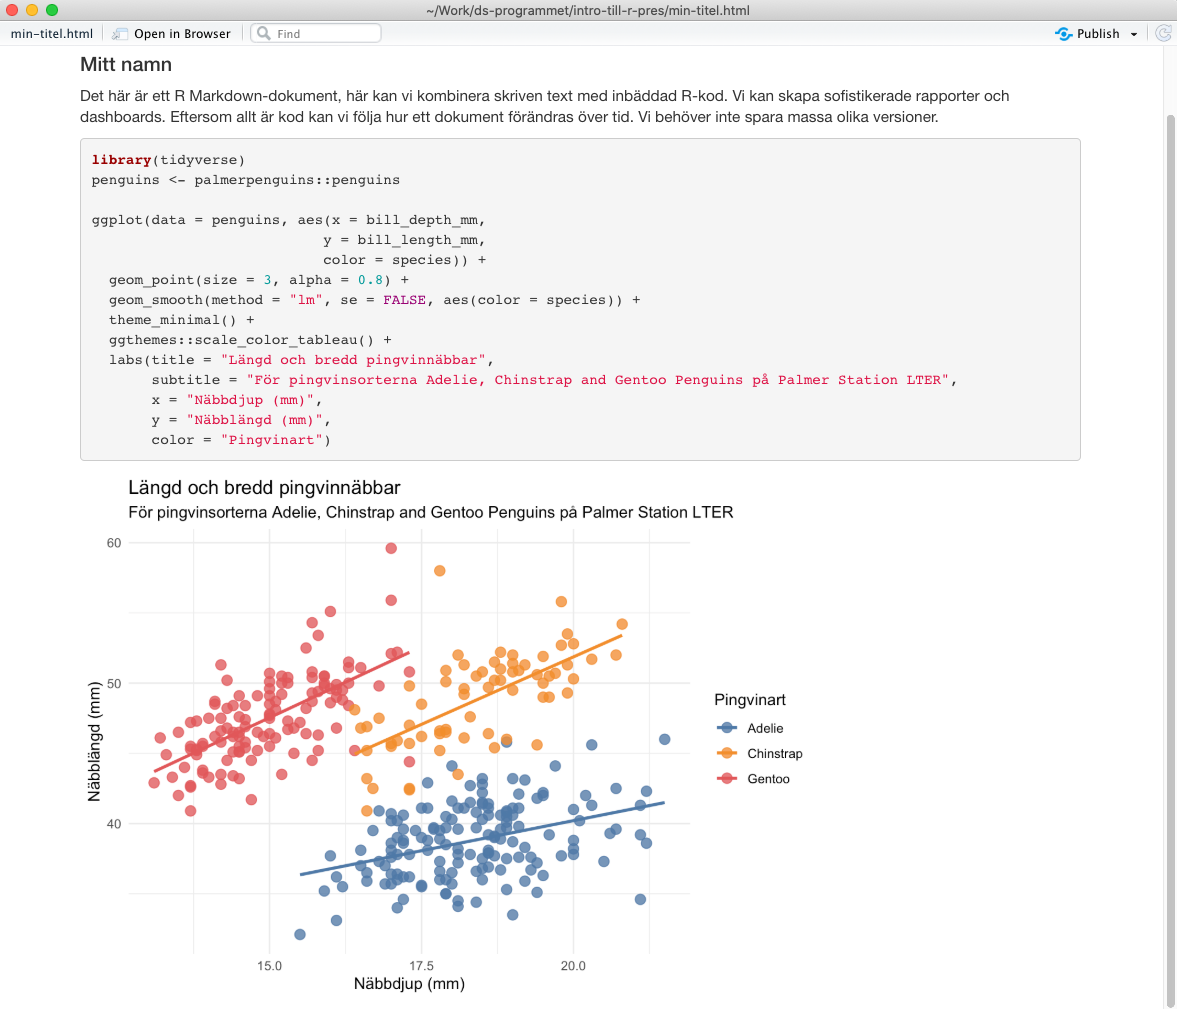
\includegraphics{images/rmd-knitted.png}

\hypertarget{kodstil-att-skriva-kod-i-r}{%
\section{Kodstil: Att skriva kod i R}\label{kodstil-att-skriva-kod-i-r}}

När du skriver kod gör du det dels med hänsyn dels till andra men framför allt med hänsyn till ditt framtida jag. Koden ska med andra ord vara enkel att läsa.

Därför kan det vara bra att följa en stilguide.

Jag följer stilguiden från \texttt{tidyverse} som säger att:

\begin{itemize}
\tightlist
\item
  Namnge alltid variabler, objekt m.m. med små bokstäver.
\end{itemize}

Exempelvis är det enklare att läsa:

\begin{Shaded}
\begin{Highlighting}[]
\NormalTok{min\_egna\_funktion }\OtherTok{\textless{}{-}} \ControlFlowTok{function}\NormalTok{(x)}
\end{Highlighting}
\end{Shaded}

I kontrast till:

\begin{Shaded}
\begin{Highlighting}[]
\NormalTok{MinEgnaFunktion }\OtherTok{\textless{}{-}} \ControlFlowTok{function}\NormalTok{(x)}
\end{Highlighting}
\end{Shaded}

Vi strävar dessutom efter att skriva kod som vi skriver text, med mellanrum mellan \texttt{,} och ord.

Det här är enklare att läsa:

\begin{Shaded}
\begin{Highlighting}[]
\FunctionTok{mean}\NormalTok{(x, }\AttributeTok{na.rm =} \ConstantTok{TRUE}\NormalTok{)}
\end{Highlighting}
\end{Shaded}

Än det här:

\begin{Shaded}
\begin{Highlighting}[]
\FunctionTok{mean}\NormalTok{(x,}\AttributeTok{na.rm=}\ConstantTok{TRUE}\NormalTok{)}
\end{Highlighting}
\end{Shaded}

När vi sparar filer så försöker vi följa den här syntaxen. Därför ska du inte ha mellanrum i när du sparar filer. \texttt{min-r-fil.R} är bra men \texttt{min\ R\ fil.R} är dåligt.

När vi skriver kod försöker vi dessutom inte att skriva för lång uttryck:

Det här är mycket svårare att läsa:

\begin{Shaded}
\begin{Highlighting}[]
\NormalTok{iris }\SpecialCharTok{\%\textgreater{}\%} \FunctionTok{group\_by}\NormalTok{(Species) }\SpecialCharTok{\%\textgreater{}\%} \FunctionTok{summarise}\NormalTok{(}\AttributeTok{Sepal.Length =} \FunctionTok{mean}\NormalTok{(Sepal.Length), }\AttributeTok{Sepal.Width =} \FunctionTok{mean}\NormalTok{(Sepal.Width), }\AttributeTok{Species =} \FunctionTok{n\_distinct}\NormalTok{(Species))}
\end{Highlighting}
\end{Shaded}

Än det här:

\begin{Shaded}
\begin{Highlighting}[]
\NormalTok{iris }\SpecialCharTok{\%\textgreater{}\%}
  \FunctionTok{group\_by}\NormalTok{(Species) }\SpecialCharTok{\%\textgreater{}\%}
  \FunctionTok{summarise}\NormalTok{(}
    \AttributeTok{Sepal.Length =} \FunctionTok{mean}\NormalTok{(Sepal.Length),}
    \AttributeTok{Sepal.Width =} \FunctionTok{mean}\NormalTok{(Sepal.Width),}
    \AttributeTok{Species =} \FunctionTok{n\_distinct}\NormalTok{(Species)}
\NormalTok{  ) }
\end{Highlighting}
\end{Shaded}

\hypertarget{databearbetning}{%
\chapter{Datamanipulering med dplyr}\label{databearbetning}}

Det sägs ofta att en Data Scientist ägnar 80\% av sin tid till att manipulera data så att den går att visualisera och modellera. Därför är det klokt att välja en metod och ett paket som underlättar det arbetet för dig.

I den här introduktionen kommer vi att fokusera på att använda paketet \texttt{dplyr} för att göra datamanipuleringar. \texttt{dplyr} är ett av de mest populära paketen i R och ger dig en bred verktygslåda för att manipulera data. \texttt{dplyr} ingår också i ett samlingspaket \texttt{tidyverse} och samlar flertalet paket för datamanipulering, visualisering och modellering.

\texttt{dplyr} har ett antal \emph{verb} för att göra manipuleringar:

\begin{itemize}
\tightlist
\item
  \textbf{\texttt{filter()}} där du väljer observationer baserat på deras värden
\item
  \textbf{\texttt{arrange()}} som ändrar ordningen på rader
\item
  \textbf{\texttt{select()}} för att välja variabler baserat på deras namn
\item
  \textbf{\texttt{mutate()}} för att skapa nya variabler baserat på funktioner
\item
  \textbf{\texttt{summarise()}} för att summera många värden till ett värde
\end{itemize}

Samtliga av dessa verb kan användas i kombination med funktionen \texttt{group\_by()} som innebär att du utför verben på flera grupper.

Alla verb i \texttt{dplyr} är konsekventa. Det första argumentet är din data och i det andra argumentet specificerar du vad du vill göra med din data. Resultatet är alltid en ny data.frame.

\hypertarget{filter}{%
\section{Filter}\label{filter}}

Med filter kan du enkelt filtrera din data baserat på villkor.

Dessa villkor uttrycks med hjälp av \texttt{relationsoperatorer} och \texttt{logical\ operators}.

I R är dessa:

\begin{tabular}{l|l}
\hline
Relationsoperator & Symbol i R\\
\hline
och (and) & \&\\
\hline
eller(or) & |\\
\hline
icke(not) & !\\
\hline
\end{tabular}

\begin{tabular}{l|l}
\hline
Logical Operators & Symbol i R\\
\hline
lika & ==\\
\hline
inte lika & !=\\
\hline
större än eller lika & >=\\
\hline
mindre än eller lika & <=\\
\hline
större än & >\\
\hline
mindre än & <\\
\hline
finns i & \%in\%\\
\hline
\end{tabular}

Dessa kan du använda i \texttt{filter()}.

\textbf{PS: Det vanligaste misstaget i början av din R-karriär är att skriva \texttt{=} istället för \texttt{==}.}

Så här använder du operatorerna:

Hitta alla flyg som kom fram 08:30 under februari

\begin{Shaded}
\begin{Highlighting}[]
\FunctionTok{library}\NormalTok{(dplyr)}
\FunctionTok{library}\NormalTok{(nycflights13)}
\FunctionTok{filter}\NormalTok{(flights, month }\SpecialCharTok{==} \DecValTok{2}\NormalTok{, arr\_time }\SpecialCharTok{==} \DecValTok{830}\NormalTok{)}
\end{Highlighting}
\end{Shaded}

\begin{verbatim}
## # A tibble: 9 x 19
##    year month   day dep_time sched_dep_time dep_delay arr_time sched_arr_time
##   <int> <int> <int>    <int>          <int>     <dbl>    <int>          <int>
## 1  2013     2     2      656            700        -4      830            839
## 2  2013     2     4      652            600        52      830            759
## 3  2013     2     6      629            630        -1      830            845
## 4  2013     2    13      633            636        -3      830            808
## 5  2013     2    18      717            700        17      830            832
## 6  2013     2    24      557            600        -3      830            837
## 7  2013     2    25      532            540        -8      830            850
## 8  2013     2    26      615            615         0      830            820
## 9  2013     2    28      621            630        -9      830            830
## # ... with 11 more variables: arr_delay <dbl>, carrier <chr>, flight <int>,
## #   tailnum <chr>, origin <chr>, dest <chr>, air_time <dbl>, distance <dbl>,
## #   hour <dbl>, minute <dbl>, time_hour <dttm>
\end{verbatim}

Hitta alla flygbolag som finns i \texttt{c("UA",\ "DL")} i februari eller mars och som inte var försenade.

\begin{Shaded}
\begin{Highlighting}[]
\FunctionTok{filter}\NormalTok{(flights, carrier }\SpecialCharTok{\%in\%} \FunctionTok{c}\NormalTok{(}\StringTok{"UA"}\NormalTok{, }\StringTok{"DL"}\NormalTok{), month }\SpecialCharTok{==} \DecValTok{2} \SpecialCharTok{|}\NormalTok{ month }\SpecialCharTok{==} \DecValTok{3}\NormalTok{, dep\_delay }\SpecialCharTok{\textless{}=} \DecValTok{0}\NormalTok{)}
\end{Highlighting}
\end{Shaded}

\begin{verbatim}
## # A tibble: 10,346 x 19
##     year month   day dep_time sched_dep_time dep_delay arr_time sched_arr_time
##    <int> <int> <int>    <int>          <int>     <dbl>    <int>          <int>
##  1  2013     2     1      520            525        -5      816            820
##  2  2013     2     1      527            530        -3      837            829
##  3  2013     2     1      554            601        -7      920            918
##  4  2013     2     1      558            600        -2      738            759
##  5  2013     2     1      559            600        -1      923            925
##  6  2013     2     1      600            600         0      833            837
##  7  2013     2     1      601            608        -7      703            725
##  8  2013     2     1      601            608        -7      723            755
##  9  2013     2     1      604            610        -6      752            817
## 10  2013     2     1      608            615        -7      837            842
## # ... with 10,336 more rows, and 11 more variables: arr_delay <dbl>,
## #   carrier <chr>, flight <int>, tailnum <chr>, origin <chr>, dest <chr>,
## #   air_time <dbl>, distance <dbl>, hour <dbl>, minute <dbl>, time_hour <dttm>
\end{verbatim}

\hypertarget{uxf6vning}{%
\subsection{Övning}\label{uxf6vning}}

\begin{itemize}
\item
  Öppna dokumentet \texttt{databearbetning-övningar.Rmd}
\item
  Börja med att ladda \texttt{tidyverse} och \texttt{nycflights13}
\item
  Spara \texttt{flights} som en data.frame i din \texttt{environment}, genom \texttt{flights\ \textless{}-\ flights}
\end{itemize}

PS. \texttt{flights} är en \texttt{tibble} som bara är en lite snyggare variant av en \texttt{data.frame}.

Nu till övningarna:

Hur många plan\ldots{}

\begin{enumerate}
\def\labelenumi{\arabic{enumi}.}
\tightlist
\item
  var försenade mer än 1 timme?
\item
  skulle till Boston (``BOS'')
\item
  lämnade JFK och var försenade
\item
  lämnade JFK på julafton
\item
  var försenade, men inte kom fram försent
\item
  flög United Airlines (UA) eller American Airlines?
\end{enumerate}

\hypertarget{arrange}{%
\section{Arrange}\label{arrange}}

\texttt{arrange()} kastar om ordningen på dina rader enligt en av dig vald variabel. Exempelvis kanske vi vill sortera data på försenade avgångar \texttt{dep\_delay}.

\begin{Shaded}
\begin{Highlighting}[]
\FunctionTok{arrange}\NormalTok{(flights, dep\_delay)}
\end{Highlighting}
\end{Shaded}

\begin{verbatim}
## # A tibble: 336,776 x 19
##     year month   day dep_time sched_dep_time dep_delay arr_time sched_arr_time
##    <int> <int> <int>    <int>          <int>     <dbl>    <int>          <int>
##  1  2013    12     7     2040           2123       -43       40           2352
##  2  2013     2     3     2022           2055       -33     2240           2338
##  3  2013    11    10     1408           1440       -32     1549           1559
##  4  2013     1    11     1900           1930       -30     2233           2243
##  5  2013     1    29     1703           1730       -27     1947           1957
##  6  2013     8     9      729            755       -26     1002            955
##  7  2013    10    23     1907           1932       -25     2143           2143
##  8  2013     3    30     2030           2055       -25     2213           2250
##  9  2013     3     2     1431           1455       -24     1601           1631
## 10  2013     5     5      934            958       -24     1225           1309
## # ... with 336,766 more rows, and 11 more variables: arr_delay <dbl>,
## #   carrier <chr>, flight <int>, tailnum <chr>, origin <chr>, dest <chr>,
## #   air_time <dbl>, distance <dbl>, hour <dbl>, minute <dbl>, time_hour <dttm>
\end{verbatim}

\texttt{arrange()} sorterar per default på sjunkande värde (ascending). Vill du sortera på stigande värde (descending) sätter du \texttt{desc()} runt din variabel.

\begin{Shaded}
\begin{Highlighting}[]
\FunctionTok{arrange}\NormalTok{(flights, }\FunctionTok{desc}\NormalTok{(dep\_delay))}
\end{Highlighting}
\end{Shaded}

\begin{verbatim}
## # A tibble: 336,776 x 19
##     year month   day dep_time sched_dep_time dep_delay arr_time sched_arr_time
##    <int> <int> <int>    <int>          <int>     <dbl>    <int>          <int>
##  1  2013     1     9      641            900      1301     1242           1530
##  2  2013     6    15     1432           1935      1137     1607           2120
##  3  2013     1    10     1121           1635      1126     1239           1810
##  4  2013     9    20     1139           1845      1014     1457           2210
##  5  2013     7    22      845           1600      1005     1044           1815
##  6  2013     4    10     1100           1900       960     1342           2211
##  7  2013     3    17     2321            810       911      135           1020
##  8  2013     6    27      959           1900       899     1236           2226
##  9  2013     7    22     2257            759       898      121           1026
## 10  2013    12     5      756           1700       896     1058           2020
## # ... with 336,766 more rows, and 11 more variables: arr_delay <dbl>,
## #   carrier <chr>, flight <int>, tailnum <chr>, origin <chr>, dest <chr>,
## #   air_time <dbl>, distance <dbl>, hour <dbl>, minute <dbl>, time_hour <dttm>
\end{verbatim}

\hypertarget{uxf6vning-1}{%
\subsection{Övning}\label{uxf6vning-1}}

Hitta det flyg som\ldots{}

\begin{enumerate}
\def\labelenumi{\arabic{enumi}.}
\tightlist
\item
  flög längst
\item
  var mest försenat (när det kom fram)
\end{enumerate}

\hypertarget{select}{%
\section{Select}\label{select}}

Medan \texttt{arrange()} kastar om raderna så kastar \texttt{select()} om kolumnerna. Men mest används den för att välja ut kolumner av intresse.

\begin{Shaded}
\begin{Highlighting}[]
\FunctionTok{select}\NormalTok{(flights, dep\_delay, carrier)}
\end{Highlighting}
\end{Shaded}

\begin{verbatim}
## # A tibble: 336,776 x 2
##    dep_delay carrier
##        <dbl> <chr>  
##  1         2 UA     
##  2         4 UA     
##  3         2 AA     
##  4        -1 B6     
##  5        -6 DL     
##  6        -4 UA     
##  7        -5 B6     
##  8        -3 EV     
##  9        -3 B6     
## 10        -2 AA     
## # ... with 336,766 more rows
\end{verbatim}

Om du av något skäl vill flytta en kolumn till början kan du skriva:

\begin{Shaded}
\begin{Highlighting}[]
\FunctionTok{select}\NormalTok{(flights, carrier, }\FunctionTok{everything}\NormalTok{())}
\end{Highlighting}
\end{Shaded}

\begin{verbatim}
## # A tibble: 336,776 x 19
##    carrier  year month   day dep_time sched_dep_time dep_delay arr_time
##    <chr>   <int> <int> <int>    <int>          <int>     <dbl>    <int>
##  1 UA       2013     1     1      517            515         2      830
##  2 UA       2013     1     1      533            529         4      850
##  3 AA       2013     1     1      542            540         2      923
##  4 B6       2013     1     1      544            545        -1     1004
##  5 DL       2013     1     1      554            600        -6      812
##  6 UA       2013     1     1      554            558        -4      740
##  7 B6       2013     1     1      555            600        -5      913
##  8 EV       2013     1     1      557            600        -3      709
##  9 B6       2013     1     1      557            600        -3      838
## 10 AA       2013     1     1      558            600        -2      753
## # ... with 336,766 more rows, and 11 more variables: sched_arr_time <int>,
## #   arr_delay <dbl>, flight <int>, tailnum <chr>, origin <chr>, dest <chr>,
## #   air_time <dbl>, distance <dbl>, hour <dbl>, minute <dbl>, time_hour <dttm>
\end{verbatim}

Du kan även välja alla kolumner mellan två kolumner:

\begin{Shaded}
\begin{Highlighting}[]
\FunctionTok{select}\NormalTok{(flights, year}\SpecialCharTok{:}\NormalTok{day)}
\end{Highlighting}
\end{Shaded}

\begin{verbatim}
## # A tibble: 336,776 x 3
##     year month   day
##    <int> <int> <int>
##  1  2013     1     1
##  2  2013     1     1
##  3  2013     1     1
##  4  2013     1     1
##  5  2013     1     1
##  6  2013     1     1
##  7  2013     1     1
##  8  2013     1     1
##  9  2013     1     1
## 10  2013     1     1
## # ... with 336,766 more rows
\end{verbatim}

Genom att sätta ett minus framför variabelnamnet exkluderar du variabeln.

\begin{Shaded}
\begin{Highlighting}[]
\FunctionTok{select}\NormalTok{(flights, }\SpecialCharTok{{-}}\NormalTok{year)}
\end{Highlighting}
\end{Shaded}

\begin{verbatim}
## # A tibble: 336,776 x 18
##    month   day dep_time sched_dep_time dep_delay arr_time sched_arr_time
##    <int> <int>    <int>          <int>     <dbl>    <int>          <int>
##  1     1     1      517            515         2      830            819
##  2     1     1      533            529         4      850            830
##  3     1     1      542            540         2      923            850
##  4     1     1      544            545        -1     1004           1022
##  5     1     1      554            600        -6      812            837
##  6     1     1      554            558        -4      740            728
##  7     1     1      555            600        -5      913            854
##  8     1     1      557            600        -3      709            723
##  9     1     1      557            600        -3      838            846
## 10     1     1      558            600        -2      753            745
## # ... with 336,766 more rows, and 11 more variables: arr_delay <dbl>,
## #   carrier <chr>, flight <int>, tailnum <chr>, origin <chr>, dest <chr>,
## #   air_time <dbl>, distance <dbl>, hour <dbl>, minute <dbl>, time_hour <dttm>
\end{verbatim}

\hypertarget{select-plus-hjuxe4lpfunktioner}{%
\subsubsection{select() plus hjälpfunktioner}\label{select-plus-hjuxe4lpfunktioner}}

\texttt{select()} kommer med ett antal hjälpfunktioner:

\begin{itemize}
\tightlist
\item
  \texttt{starts\_with("asd")}
\item
  \texttt{ends\_with("air")}
\item
  \texttt{contains("flyg")}
\item
  \texttt{matches("asd")}
\item
  \texttt{num\_range("flyg",\ 1:10)}
\end{itemize}

De används för att identifiera kolumner baserat på text.

Exempelvis kan du hitta alla delay-kolumner med \texttt{contains}.

\begin{Shaded}
\begin{Highlighting}[]
\FunctionTok{select}\NormalTok{(flights, }\FunctionTok{contains}\NormalTok{(}\StringTok{"delay"}\NormalTok{))}
\end{Highlighting}
\end{Shaded}

\begin{verbatim}
## # A tibble: 336,776 x 2
##    dep_delay arr_delay
##        <dbl>     <dbl>
##  1         2        11
##  2         4        20
##  3         2        33
##  4        -1       -18
##  5        -6       -25
##  6        -4        12
##  7        -5        19
##  8        -3       -14
##  9        -3        -8
## 10        -2         8
## # ... with 336,766 more rows
\end{verbatim}

\hypertarget{rename}{%
\subsubsection{rename()}\label{rename}}

En annan nyttig funktion är \texttt{rename()} som kort och gott döper om variabler.

Formeln är \texttt{rename(data,\ ny\_variabel\ =\ gammal\_variabel)}

\hypertarget{uxf6vning-2}{%
\subsection{Övning}\label{uxf6vning-2}}

\begin{enumerate}
\def\labelenumi{\arabic{enumi}.}
\item
  Som innehåller ``dep''
\item
  Som börjar med ``dep''
\item
  Som är numeriska
\item
  Döp om \texttt{dep\_delay} till \texttt{försenad\_avgång}
\end{enumerate}

\hypertarget{kallad-the-pipe}{%
\section{\texorpdfstring{\texttt{\%\textgreater{}\%} kallad ``the pipe''}{\%\textgreater\% kallad ``the pipe''}}\label{kallad-the-pipe}}

\begin{itemize}
\item
  Används för att länka ihop flera uttryck i \emph{R}.
\item
  \texttt{ctrl\ +\ shift\ +\ m} (i Windows) och \texttt{ctrl\ +\ command\ +\ m} (Mac)
\end{itemize}

\begin{Shaded}
\begin{Highlighting}[]
\NormalTok{flights }\SpecialCharTok{\%\textgreater{}\%} 
  \FunctionTok{filter}\NormalTok{(month }\SpecialCharTok{==} \DecValTok{2}\NormalTok{, arr\_time }\SpecialCharTok{==} \DecValTok{830}\NormalTok{) }\SpecialCharTok{\%\textgreater{}\%} 
  \FunctionTok{select}\NormalTok{(dest, year, month, day, arr\_time)}
\end{Highlighting}
\end{Shaded}

\begin{verbatim}
## # A tibble: 9 x 5
##   dest   year month   day arr_time
##   <chr> <int> <int> <int>    <int>
## 1 ORD    2013     2     2      830
## 2 DTW    2013     2     4      830
## 3 CLT    2013     2     6      830
## 4 BNA    2013     2    13      830
## 5 BNA    2013     2    18      830
## 6 ATL    2013     2    24      830
## 7 MIA    2013     2    25      830
## 8 CLT    2013     2    26      830
## 9 CLT    2013     2    28      830
\end{verbatim}

\hypertarget{mutate}{%
\section{Mutate}\label{mutate}}

\texttt{mutate()} används för att skapa nya variabler.

Exempelvis kan vi räkna ut hur mycket tid man vunnit om exempelvis flyget landar tidigare än avsett.

\begin{Shaded}
\begin{Highlighting}[]
\NormalTok{flights }\SpecialCharTok{\%\textgreater{}\%} 
  \FunctionTok{mutate}\NormalTok{(}\AttributeTok{beer\_time =}\NormalTok{ dep\_delay }\SpecialCharTok{{-}}\NormalTok{ arr\_delay)}
\end{Highlighting}
\end{Shaded}

\begin{verbatim}
## # A tibble: 336,776 x 20
##     year month   day dep_time sched_dep_time dep_delay arr_time sched_arr_time
##    <int> <int> <int>    <int>          <int>     <dbl>    <int>          <int>
##  1  2013     1     1      517            515         2      830            819
##  2  2013     1     1      533            529         4      850            830
##  3  2013     1     1      542            540         2      923            850
##  4  2013     1     1      544            545        -1     1004           1022
##  5  2013     1     1      554            600        -6      812            837
##  6  2013     1     1      554            558        -4      740            728
##  7  2013     1     1      555            600        -5      913            854
##  8  2013     1     1      557            600        -3      709            723
##  9  2013     1     1      557            600        -3      838            846
## 10  2013     1     1      558            600        -2      753            745
## # ... with 336,766 more rows, and 12 more variables: arr_delay <dbl>,
## #   carrier <chr>, flight <int>, tailnum <chr>, origin <chr>, dest <chr>,
## #   air_time <dbl>, distance <dbl>, hour <dbl>, minute <dbl>, time_hour <dttm>,
## #   beer_time <dbl>
\end{verbatim}

\texttt{mutate()} kan användas för att slå ihop variabler

\begin{Shaded}
\begin{Highlighting}[]
\NormalTok{flights }\SpecialCharTok{\%\textgreater{}\%} 
  \FunctionTok{mutate}\NormalTok{(}\AttributeTok{date =} \FunctionTok{paste}\NormalTok{(year, month, day, }\AttributeTok{sep =} \StringTok{"{-}"}\NormalTok{)) }\SpecialCharTok{\%\textgreater{}\%} 
  \FunctionTok{select}\NormalTok{(year, month, day, date)}
\end{Highlighting}
\end{Shaded}

\begin{verbatim}
## # A tibble: 336,776 x 4
##     year month   day date    
##    <int> <int> <int> <chr>   
##  1  2013     1     1 2013-1-1
##  2  2013     1     1 2013-1-1
##  3  2013     1     1 2013-1-1
##  4  2013     1     1 2013-1-1
##  5  2013     1     1 2013-1-1
##  6  2013     1     1 2013-1-1
##  7  2013     1     1 2013-1-1
##  8  2013     1     1 2013-1-1
##  9  2013     1     1 2013-1-1
## 10  2013     1     1 2013-1-1
## # ... with 336,766 more rows
\end{verbatim}

I \texttt{mutate()} kan du även använda funktioner såsom \texttt{mean()}.

\begin{Shaded}
\begin{Highlighting}[]
\NormalTok{flights }\SpecialCharTok{\%\textgreater{}\%} 
  \FunctionTok{mutate}\NormalTok{(}\AttributeTok{mean\_delay =} \FunctionTok{mean}\NormalTok{(dep\_delay, }\AttributeTok{na.rm =}\NormalTok{ T)) }\SpecialCharTok{\%\textgreater{}\%} 
  \FunctionTok{select}\NormalTok{(year, month, day, mean\_delay)}
\end{Highlighting}
\end{Shaded}

\begin{verbatim}
## # A tibble: 336,776 x 4
##     year month   day mean_delay
##    <int> <int> <int>      <dbl>
##  1  2013     1     1       12.6
##  2  2013     1     1       12.6
##  3  2013     1     1       12.6
##  4  2013     1     1       12.6
##  5  2013     1     1       12.6
##  6  2013     1     1       12.6
##  7  2013     1     1       12.6
##  8  2013     1     1       12.6
##  9  2013     1     1       12.6
## 10  2013     1     1       12.6
## # ... with 336,766 more rows
\end{verbatim}

\hypertarget{if_else}{%
\subsection{if\_else()}\label{if_else}}

En vanlig funktion i databearbetning är ifelse-satser.

I R gör du det enklast med funktionen \texttt{if\_else()} från \texttt{dplyr}. Det finns även en inbyggd funktion som heter \texttt{ifelse()} som mestadels fungerar bra men den från \texttt{dplyr} är något mer stabil.

Du kan använda den i mutate:

\begin{Shaded}
\begin{Highlighting}[]
\FunctionTok{mutate}\NormalTok{(flights, försenad }\OtherTok{=} \FunctionTok{if\_else}\NormalTok{(dep\_delay  }\SpecialCharTok{\textgreater{}} \DecValTok{5}\NormalTok{, }\StringTok{"försenad"}\NormalTok{, }\StringTok{"ej försenad"}\NormalTok{))}
\end{Highlighting}
\end{Shaded}

\begin{verbatim}
## # A tibble: 336,776 x 20
##     year month   day dep_time sched_dep_time dep_delay arr_time sched_arr_time
##    <int> <int> <int>    <int>          <int>     <dbl>    <int>          <int>
##  1  2013     1     1      517            515         2      830            819
##  2  2013     1     1      533            529         4      850            830
##  3  2013     1     1      542            540         2      923            850
##  4  2013     1     1      544            545        -1     1004           1022
##  5  2013     1     1      554            600        -6      812            837
##  6  2013     1     1      554            558        -4      740            728
##  7  2013     1     1      555            600        -5      913            854
##  8  2013     1     1      557            600        -3      709            723
##  9  2013     1     1      557            600        -3      838            846
## 10  2013     1     1      558            600        -2      753            745
## # ... with 336,766 more rows, and 12 more variables: arr_delay <dbl>,
## #   carrier <chr>, flight <int>, tailnum <chr>, origin <chr>, dest <chr>,
## #   air_time <dbl>, distance <dbl>, hour <dbl>, minute <dbl>, time_hour <dttm>,
## #   försenad <chr>
\end{verbatim}

\hypertarget{case_when}{%
\subsection{case\_when()}\label{case_when}}

Ibland vill man göra flera stycken \texttt{if\_else()} i samma, exempelvis om man vill dela upp en variabel i flera kategorier beroende på ett logiskt villkor. För att göra det kan du använda funktionen \texttt{case\_when()}.

\begin{Shaded}
\begin{Highlighting}[]
\FunctionTok{mutate}\NormalTok{(flights, försenad}\AttributeTok{\_kat =} \FunctionTok{case\_when}\NormalTok{(}
\NormalTok{dep\_delay }\SpecialCharTok{\textless{}} \DecValTok{0} \SpecialCharTok{\textasciitilde{}} \StringTok{"före tid"}\NormalTok{,}
\NormalTok{dep\_delay }\SpecialCharTok{==} \DecValTok{0} \SpecialCharTok{\textasciitilde{}} \StringTok{"i tid"}\NormalTok{,}
\NormalTok{dep\_delay }\SpecialCharTok{\textgreater{}} \DecValTok{0} \SpecialCharTok{\textasciitilde{}} \StringTok{"försenad"}\NormalTok{)) }
\end{Highlighting}
\end{Shaded}

\begin{verbatim}
## # A tibble: 336,776 x 20
##     year month   day dep_time sched_dep_time dep_delay arr_time sched_arr_time
##    <int> <int> <int>    <int>          <int>     <dbl>    <int>          <int>
##  1  2013     1     1      517            515         2      830            819
##  2  2013     1     1      533            529         4      850            830
##  3  2013     1     1      542            540         2      923            850
##  4  2013     1     1      544            545        -1     1004           1022
##  5  2013     1     1      554            600        -6      812            837
##  6  2013     1     1      554            558        -4      740            728
##  7  2013     1     1      555            600        -5      913            854
##  8  2013     1     1      557            600        -3      709            723
##  9  2013     1     1      557            600        -3      838            846
## 10  2013     1     1      558            600        -2      753            745
## # ... with 336,766 more rows, and 12 more variables: arr_delay <dbl>,
## #   carrier <chr>, flight <int>, tailnum <chr>, origin <chr>, dest <chr>,
## #   air_time <dbl>, distance <dbl>, hour <dbl>, minute <dbl>, time_hour <dttm>,
## #   försenad_kat <chr>
\end{verbatim}

\hypertarget{andra-funktioner}{%
\subsection{Andra funktioner}\label{andra-funktioner}}

I \texttt{mutate()} kan du använda de allra flesta funktionerna i R. Här är exempel på några funktioner som kan vara nyttiga i databearbetning:

\begin{itemize}
\tightlist
\item
  Funktioner för att ranka variabler: \texttt{rank()}, \texttt{min\_rank()}, \texttt{dense\_rank()}, \texttt{percent\_rank()}
\item
  För att logaritmiska funktioner: \texttt{log()}, \texttt{log10()}
\item
  För kumulativa beräkningar: \texttt{cumsum()}, \texttt{cummean()}
\item
  För att bara generera radnummer: \texttt{row\_number()}
\item
  För att ta observation innan eller efter: \texttt{lead()} och \texttt{lag()}
\item
  För skapa variabler baserat på värde i andra variabler \texttt{if\_else()} och \texttt{case\_when()}
\end{itemize}

\hypertarget{uxf6vningar}{%
\subsection{Övningar}\label{uxf6vningar}}

\begin{enumerate}
\def\labelenumi{\arabic{enumi}.}
\item
  Skapa en variabel med \texttt{dep\_delay} \emph{minus} medelvärdet för \texttt{dep\_delay}
\item
  Rangordna flygens distans med \texttt{dense\_rank()}. Hur hanterar den distanser är lika långa? Vilka fler rankingfunktioner skulle du kunna använda? Se \texttt{?dense\_rank()}
\item
  Skapa en variabel som anger om flyget går på våren, hösten, vintern eller sommaren med \texttt{case\_when()}
\end{enumerate}

\hypertarget{summarise}{%
\section{Summarise}\label{summarise}}

Ofta vill man summera variabler för att få ut intressant information. Exempelvis vill vi här kanske veta en rad medelvärden.

\begin{Shaded}
\begin{Highlighting}[]
\NormalTok{flights }\SpecialCharTok{\%\textgreater{}\%} 
  \FunctionTok{summarise}\NormalTok{(}
    \AttributeTok{mean\_air\_time =} \FunctionTok{mean}\NormalTok{(air\_time, }\AttributeTok{na.rm =}\NormalTok{ T),}
    \AttributeTok{mean\_dep\_delay =} \FunctionTok{mean}\NormalTok{(dep\_delay, }\AttributeTok{na.rm =}\NormalTok{ T),}
    \AttributeTok{mean\_arr\_delay =} \FunctionTok{mean}\NormalTok{(arr\_delay, }\AttributeTok{na.rm =}\NormalTok{ T)}
\NormalTok{  )}
\end{Highlighting}
\end{Shaded}

\begin{verbatim}
## # A tibble: 1 x 3
##   mean_air_time mean_dep_delay mean_arr_delay
##           <dbl>          <dbl>          <dbl>
## 1          151.           12.6           6.90
\end{verbatim}

Men dessa värden är inte så intressanta i sig, utan vi vill kunna göra jämförelse. Då använder vi \texttt{group\_by()}.

\begin{Shaded}
\begin{Highlighting}[]
\NormalTok{flights }\SpecialCharTok{\%\textgreater{}\%} 
  \FunctionTok{group\_by}\NormalTok{(dest) }\SpecialCharTok{\%\textgreater{}\%}
  \FunctionTok{summarise}\NormalTok{(}\AttributeTok{mean\_air\_time =} \FunctionTok{mean}\NormalTok{(air\_time, }\AttributeTok{na.rm =}\NormalTok{ T),}
          \AttributeTok{mean\_dep\_delay =} \FunctionTok{mean}\NormalTok{(dep\_delay, }\AttributeTok{na.rm =}\NormalTok{ T),}
          \AttributeTok{mean\_arr\_delay =} \FunctionTok{mean}\NormalTok{(arr\_delay, }\AttributeTok{na.rm =}\NormalTok{ T)) }\SpecialCharTok{\%\textgreater{}\%} 
  \FunctionTok{arrange}\NormalTok{(}\FunctionTok{desc}\NormalTok{(mean\_arr\_delay))}
\end{Highlighting}
\end{Shaded}

\begin{verbatim}
## `summarise()` ungrouping output (override with `.groups` argument)
\end{verbatim}

\begin{verbatim}
## # A tibble: 105 x 4
##    dest  mean_air_time mean_dep_delay mean_arr_delay
##    <chr>         <dbl>          <dbl>          <dbl>
##  1 CAE            93.2           35.6           41.8
##  2 TUL           178.            34.9           33.7
##  3 OKC           193.            30.6           30.6
##  4 JAC           264.            26.5           28.1
##  5 TYS            97.7           28.5           24.1
##  6 MSN           123.            23.6           20.2
##  7 RIC            54.0           23.6           20.1
##  8 CAK            64.0           20.8           19.7
##  9 DSM           149.            26.2           19.0
## 10 GRR            97             19.5           18.2
## # ... with 95 more rows
\end{verbatim}

I \texttt{summarise()} kan du använda en rad olika funktioner såsom \texttt{sum()} för summeringar, \texttt{n()} för antal rader, \texttt{median()} för median etc.

\begin{Shaded}
\begin{Highlighting}[]
\NormalTok{flights }\SpecialCharTok{\%\textgreater{}\%} 
 \FunctionTok{group\_by}\NormalTok{(dest) }\SpecialCharTok{\%\textgreater{}\%} 
  \FunctionTok{summarise}\NormalTok{(}
    \AttributeTok{n\_rows =} \FunctionTok{n}\NormalTok{(),}
    \AttributeTok{sum\_air\_time =} \FunctionTok{sum}\NormalTok{(air\_time, }\AttributeTok{na.rm =}\NormalTok{ T),}
    \AttributeTok{median\_air\_time =} \FunctionTok{median}\NormalTok{(air\_time, }\AttributeTok{na.rm =}\NormalTok{ T)) }\SpecialCharTok{\%\textgreater{}\%} 
  \FunctionTok{arrange}\NormalTok{(}\FunctionTok{desc}\NormalTok{(sum\_air\_time))}
\end{Highlighting}
\end{Shaded}

\begin{verbatim}
## `summarise()` ungrouping output (override with `.groups` argument)
\end{verbatim}

\begin{verbatim}
## # A tibble: 105 x 4
##    dest  n_rows sum_air_time median_air_time
##    <chr>  <int>        <dbl>           <dbl>
##  1 LAX    16174      5258470             328
##  2 SFO    13331      4553684             345
##  3 ORD    17283      1914833             114
##  4 ATL    17215      1901410             112
##  5 MCO    14082      1882381             133
##  6 FLL    12055      1811271             151
##  7 LAS     5997      1795662             301
##  8 MIA    11728      1775327             152
##  9 DFW     8738      1667341             198
## 10 DEN     7266      1623626             225
## # ... with 95 more rows
\end{verbatim}

\hypertarget{count}{%
\subsection{count()}\label{count}}

Du kan i \texttt{summarise()} räkna antalet observationer med funktionen \texttt{n()}.

\begin{Shaded}
\begin{Highlighting}[]
\NormalTok{flights }\SpecialCharTok{\%\textgreater{}\%}
  \FunctionTok{group\_by}\NormalTok{(carrier) }\SpecialCharTok{\%\textgreater{}\%}
  \FunctionTok{summarise}\NormalTok{(}\AttributeTok{count =} \FunctionTok{n}\NormalTok{())}
\end{Highlighting}
\end{Shaded}

Men istället för att göra det här kan du använda funktionen \texttt{count()}

\begin{Shaded}
\begin{Highlighting}[]
\NormalTok{flights }\SpecialCharTok{\%\textgreater{}\%}
  \FunctionTok{group\_by}\NormalTok{(carrier) }\SpecialCharTok{\%\textgreater{}\%}
  \FunctionTok{count}\NormalTok{()}
\end{Highlighting}
\end{Shaded}

\begin{verbatim}
## # A tibble: 16 x 2
## # Groups:   carrier [16]
##    carrier     n
##    <chr>   <int>
##  1 9E      18460
##  2 AA      32729
##  3 AS        714
##  4 B6      54635
##  5 DL      48110
##  6 EV      54173
##  7 F9        685
##  8 FL       3260
##  9 HA        342
## 10 MQ      26397
## 11 OO         32
## 12 UA      58665
## 13 US      20536
## 14 VX       5162
## 15 WN      12275
## 16 YV        601
\end{verbatim}

\hypertarget{sample_n}{%
\subsection{\texorpdfstring{\texttt{sample\_n()}}{sample\_n()}}\label{sample_n}}

Att göra slumpmässiga urval är en vanlig arbetsuppgift för en data scientist. Det gör du enkelt med \texttt{sample\_n()} från \texttt{dplyr}.

Om du vill ta ett slumpmässigt urval om 10 från exempelvis \texttt{flights} gör du bara:

\begin{Shaded}
\begin{Highlighting}[]
\FunctionTok{sample\_n}\NormalTok{(flights, }\DecValTok{10}\NormalTok{)}
\end{Highlighting}
\end{Shaded}

\begin{verbatim}
## # A tibble: 10 x 19
##     year month   day dep_time sched_dep_time dep_delay arr_time sched_arr_time
##    <int> <int> <int>    <int>          <int>     <dbl>    <int>          <int>
##  1  2013     1     8     1942           1935         7     2140           2145
##  2  2013    11    20     1800           1801        -1     1946           1944
##  3  2013     2    19     1919           1855        24     2058           2100
##  4  2013     8    26     1550           1550         0     1735           1749
##  5  2013    11    11     2104           2107        -3     2218           2226
##  6  2013    10    24     1618           1615         3     1909           1915
##  7  2013     7    11     1132           1130         2     1333           1327
##  8  2013     1    21     1123           1130        -7     1412           1422
##  9  2013     3    14     1427           1415        12     1632           1631
## 10  2013     6    27     1951           1723       148       NA           2013
## # ... with 11 more variables: arr_delay <dbl>, carrier <chr>, flight <int>,
## #   tailnum <chr>, origin <chr>, dest <chr>, air_time <dbl>, distance <dbl>,
## #   hour <dbl>, minute <dbl>, time_hour <dttm>
\end{verbatim}

Om du istället vill ta ett urval som baseras på \emph{procent} kan du använda \texttt{sample\_frac}, här för \emph{0.1\%}

\begin{Shaded}
\begin{Highlighting}[]
\FunctionTok{sample\_frac}\NormalTok{(flights, }\FloatTok{0.001}\NormalTok{)}
\end{Highlighting}
\end{Shaded}

\begin{verbatim}
## # A tibble: 337 x 19
##     year month   day dep_time sched_dep_time dep_delay arr_time sched_arr_time
##    <int> <int> <int>    <int>          <int>     <dbl>    <int>          <int>
##  1  2013     5    23     2343           2159       104       52           2326
##  2  2013     9    26     1827           1829        -2     2016           2011
##  3  2013     3     9     1137           1139        -2     1430           1446
##  4  2013    10    31      840            630       130     1114            839
##  5  2013     5    22     1835           1700        95     2006           1819
##  6  2013     8     1     1344           1338         6     1642           1634
##  7  2013     1    11      757            755         2      909            930
##  8  2013     3    26     1730           1730         0     1923           1923
##  9  2013     8     5     1513           1520        -7     1705           1710
## 10  2013     8    25     1729           1735        -6     1918           1929
## # ... with 327 more rows, and 11 more variables: arr_delay <dbl>,
## #   carrier <chr>, flight <int>, tailnum <chr>, origin <chr>, dest <chr>,
## #   air_time <dbl>, distance <dbl>, hour <dbl>, minute <dbl>, time_hour <dttm>
\end{verbatim}

\hypertarget{uxf6vningar-1}{%
\subsubsection{Övningar}\label{uxf6vningar-1}}

\begin{enumerate}
\def\labelenumi{\arabic{enumi}.}
\tightlist
\item
  Vilken flygplats har högst medelvärde förförseningar från flygplatsen?
\item
  Vilken flygplats tar emot minst flyg?
\end{enumerate}

\hypertarget{uxf6vning---vuxe4v-ihop-allt-du-luxe4rt-dig}{%
\subsection{Övning - väv ihop allt du lärt dig}\label{uxf6vning---vuxe4v-ihop-allt-du-luxe4rt-dig}}

\begin{enumerate}
\def\labelenumi{\arabic{enumi}.}
\tightlist
\item
  Vilken månad ska du flyga under för att undvika förseningar?
\item
  Vilken tid ska du flyga för att undvika förseningar?
\item
  Hitta det flygbolag som flyger till flest destinationer, rangordna flygbolagen baserat på den informationen.
\end{enumerate}

\hypertarget{eda}{%
\chapter{Explorativ dataanalys}\label{eda}}

\hypertarget{vad-uxe4r-explorativ-dataanalys}{%
\section{Vad är Explorativ Dataanalys?}\label{vad-uxe4r-explorativ-dataanalys}}

\begin{itemize}
\item
  En kreativ iterativ process där man ställer frågor/gör hypoteser om sin data och sedan utforskar dem
\item
  Mera konkret kan det beskrivas som
\end{itemize}

\begin{enumerate}
\def\labelenumi{\arabic{enumi}.}
\tightlist
\item
  Formulera en hypotes
\item
  Transformera din data - om nödvändigt
\item
  Visualisera din data (vårt fokus idag)
\item
  Modellera - om nödvändigt
\item
  Formulera nya hypoteser
\end{enumerate}

\begin{itemize}
\item
  Mindset inte formel!
\item
\end{itemize}

\hypertarget{exempel-puxe5-basala-fruxe5gorhypoteser}{%
\subsection{Exempel på basala frågor/hypoteser}\label{exempel-puxe5-basala-fruxe5gorhypoteser}}

Frågeställningar kan vara vaga!

\begin{itemize}
\item
  Vad för data innehåller de olika kolonnerna?
\item
  Hur ser Datans kvalitét ut? e.g missing values, felaktiga tabellvärden, duplicerade värden
\item
  Finns det outliers?
\item
  Medelvärde, spridning
\item
\end{itemize}

\hypertarget{hur-guxf6r-man-i-r}{%
\subsection{Hur gör man i R?}\label{hur-guxf6r-man-i-r}}

R har basfunktionalitet som kan användas för att snabbt få en numerisk överblick datan t.ex
\texttt{summary()} och \texttt{head()}

\begin{Shaded}
\begin{Highlighting}[]
\FunctionTok{summary}\NormalTok{(iris)}
\end{Highlighting}
\end{Shaded}

\begin{verbatim}
##   Sepal.Length    Sepal.Width     Petal.Length    Petal.Width   
##  Min.   :4.300   Min.   :2.000   Min.   :1.000   Min.   :0.100  
##  1st Qu.:5.100   1st Qu.:2.800   1st Qu.:1.600   1st Qu.:0.300  
##  Median :5.800   Median :3.000   Median :4.350   Median :1.300  
##  Mean   :5.843   Mean   :3.057   Mean   :3.758   Mean   :1.199  
##  3rd Qu.:6.400   3rd Qu.:3.300   3rd Qu.:5.100   3rd Qu.:1.800  
##  Max.   :7.900   Max.   :4.400   Max.   :6.900   Max.   :2.500  
##        Species  
##  setosa    :50  
##  versicolor:50  
##  virginica :50  
##                 
##                 
## 
\end{verbatim}

\begin{Shaded}
\begin{Highlighting}[]
\FunctionTok{head}\NormalTok{(iris)}
\end{Highlighting}
\end{Shaded}

\begin{verbatim}
##   Sepal.Length Sepal.Width Petal.Length Petal.Width Species
## 1          5.1         3.5          1.4         0.2  setosa
## 2          4.9         3.0          1.4         0.2  setosa
## 3          4.7         3.2          1.3         0.2  setosa
## 4          4.6         3.1          1.5         0.2  setosa
## 5          5.0         3.6          1.4         0.2  setosa
## 6          5.4         3.9          1.7         0.4  setosa
\end{verbatim}

\hypertarget{hur-guxf6r-man-i-r-1}{%
\subsection{Hur gör man i R?}\label{hur-guxf6r-man-i-r-1}}

R har även mer avancerade verktyg:
- \texttt{dlookr}, ta fram rapport för datakvalitét

\begin{itemize}
\tightlist
\item
  \texttt{skimr}, snabb explorativ analys (som vi kommer använda idag)
\end{itemize}

\begin{Shaded}
\begin{Highlighting}[]
\FunctionTok{skim}\NormalTok{(iris)}
\end{Highlighting}
\end{Shaded}

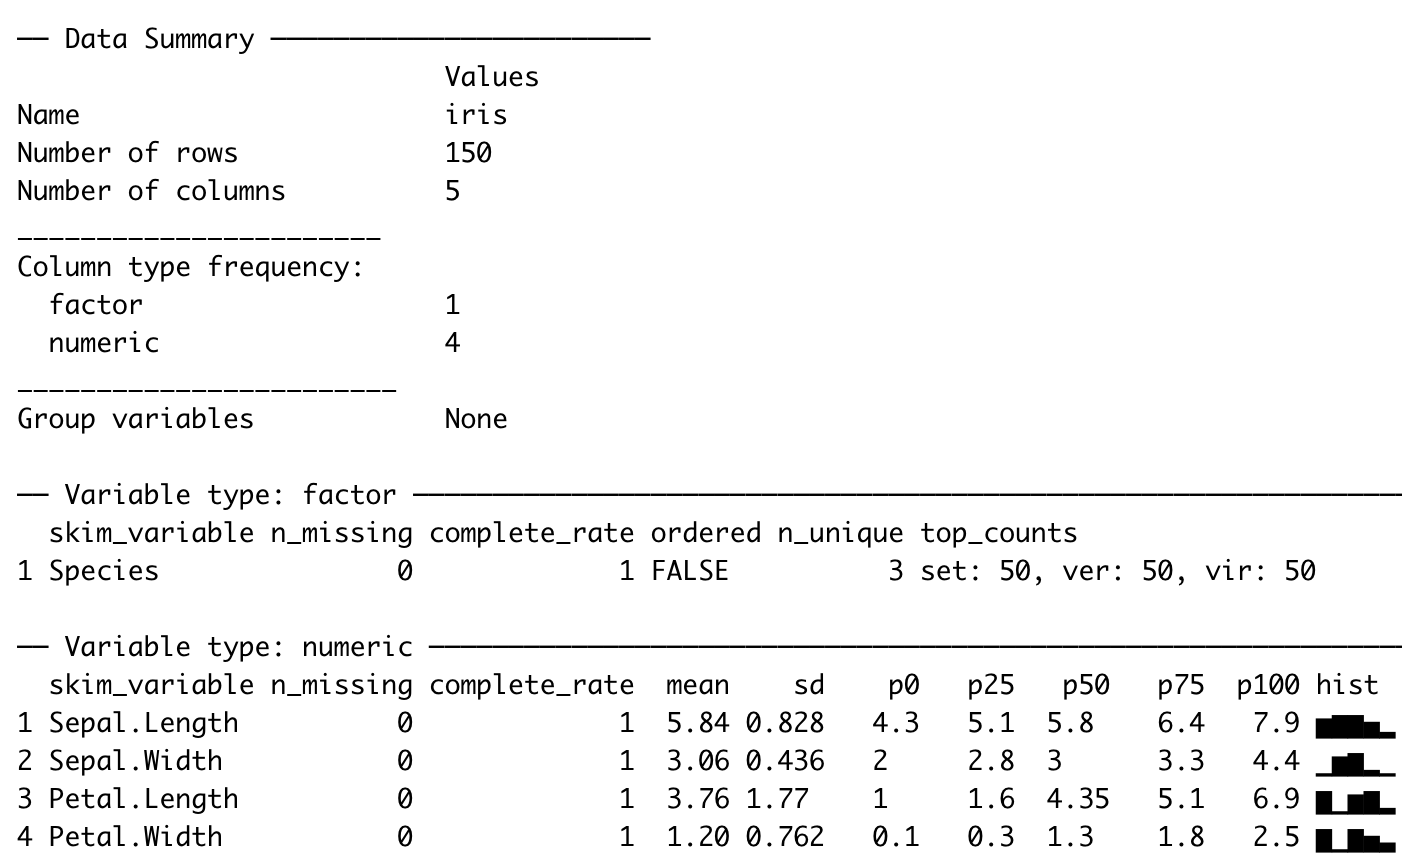
\includegraphics{images/Iris_skim.png}

\hypertarget{datavisualisering}{%
\section{Datavisualisering}\label{datavisualisering}}

\begin{itemize}
\item
  Grunden i explorativ dataanalys
\item
  Visualisering är grundläggande för att människor ska kunna få en överblick av data
\end{itemize}

\hypertarget{varfuxf6r-visualisera}{%
\subsection{Varför visualisera?}\label{varfuxf6r-visualisera}}

Anscombe quartet - Dataset skapat av Francis Anscombe 1973

\begin{verbatim}
##    observation set  x    y
## 1            1   I 10 8.04
## 2            1  II 10 9.14
## 3            1 III 10 7.46
## 4            1  IV  8 6.58
## 5            2   I  8 6.95
## 6            2  II  8 8.14
## 7            2 III  8 6.77
## 8            2  IV  8 5.76
## 9            3   I 13 7.58
## 10           3  II 13 8.74
\end{verbatim}

\hypertarget{vad-uxe4r-det-fuxf6rsta-vi-guxf6r}{%
\subsection{Vad är det första vi gör?}\label{vad-uxe4r-det-fuxf6rsta-vi-guxf6r}}

\begin{verbatim}
## # A tibble: 4 x 5
##   set   x_mean y_mean  x_sd  y_sd
##   <chr>  <dbl>  <dbl> <dbl> <dbl>
## 1 I          9   7.50  3.32  2.03
## 2 II         9   7.50  3.32  2.03
## 3 III        9   7.5   3.32  2.03
## 4 IV         9   7.50  3.32  2.03
\end{verbatim}

Ser bra ut!

\hypertarget{steg-2-anpassar-en-linjuxe4r-modell}{%
\subsection{Steg 2: anpassar en linjär modell}\label{steg-2-anpassar-en-linjuxe4r-modell}}

\begin{Shaded}
\begin{Highlighting}[]
\NormalTok{anscombe\_tidy }\SpecialCharTok{\%\textgreater{}\%} 
  \FunctionTok{nest}\NormalTok{(observation, x, y) }\SpecialCharTok{\%\textgreater{}\%} 
  \FunctionTok{mutate}\NormalTok{(}\AttributeTok{model =} \FunctionTok{map}\NormalTok{(data, }\SpecialCharTok{\textasciitilde{}}\FunctionTok{lm}\NormalTok{(y }\SpecialCharTok{\textasciitilde{}}\NormalTok{ x, }\AttributeTok{data =}\NormalTok{ .x)),}
         \AttributeTok{tidy =} \FunctionTok{map}\NormalTok{(model, broom}\SpecialCharTok{::}\NormalTok{tidy)) }\SpecialCharTok{\%\textgreater{}\%} 
  \FunctionTok{unnest}\NormalTok{(tidy) }\SpecialCharTok{\%\textgreater{}\%} 
  \FunctionTok{filter}\NormalTok{(term }\SpecialCharTok{==} \StringTok{"x"}\NormalTok{) }\SpecialCharTok{\%\textgreater{}\%} 
  \FunctionTok{select}\NormalTok{(set, estimate, std.error, statistic)}
\end{Highlighting}
\end{Shaded}

\begin{verbatim}
## Warning: All elements of `...` must be named.
## Did you want `data = c(observation, x, y)`?
\end{verbatim}

\begin{verbatim}
## # A tibble: 4 x 4
##   set   estimate std.error statistic
##   <chr>    <dbl>     <dbl>     <dbl>
## 1 I        0.500     0.118      4.24
## 2 II       0.5       0.118      4.24
## 3 III      0.500     0.118      4.24
## 4 IV       0.500     0.118      4.24
\end{verbatim}

Ser inte ut som att det är någon skillnad mellan grupperna

Men\ldots{}

\begin{verbatim}
## `geom_smooth()` using formula 'y ~ x'
\end{verbatim}

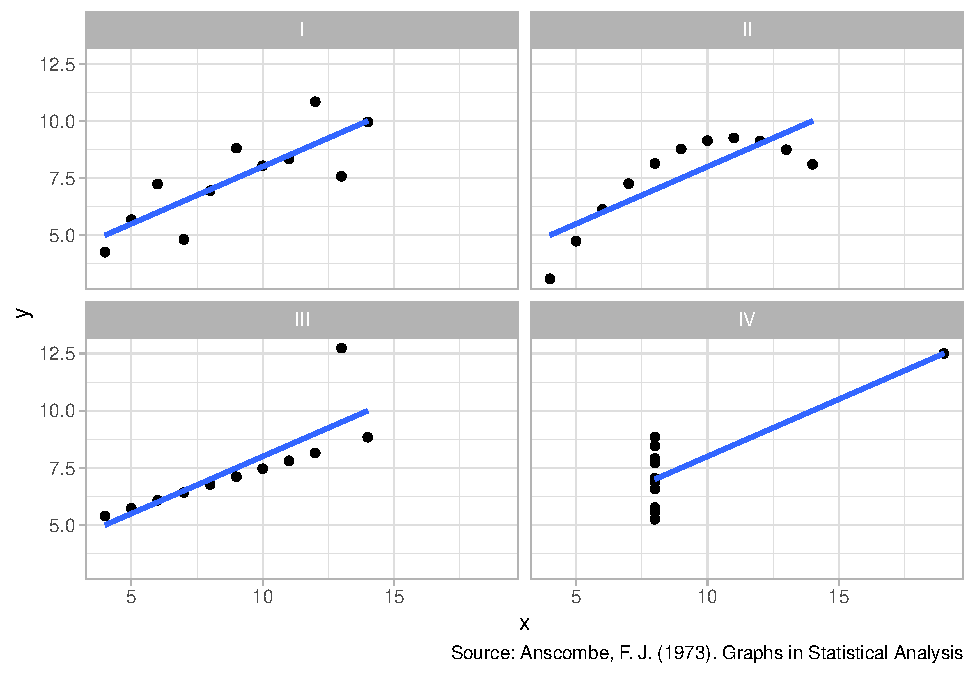
\includegraphics{ds-intro-till-r-bok_files/figure-latex/anscombe_final-1.pdf}

Statistiska mått kan gömma mycket av sanningen!

\hypertarget{datasaurus-dozen}{%
\section{Datasaurus Dozen}\label{datasaurus-dozen}}

Modern variant av Anscombe - skapat av Alberto Cairo

\begin{Shaded}
\begin{Highlighting}[]
\FunctionTok{library}\NormalTok{(datasauRus)}
\NormalTok{datasaurus\_dozen }\SpecialCharTok{\%\textgreater{}\%} 
  \FunctionTok{group\_by}\NormalTok{(dataset) }\SpecialCharTok{\%\textgreater{}\%}
  \FunctionTok{summarise}\NormalTok{(}\AttributeTok{x\_mean =} \FunctionTok{mean}\NormalTok{(x), }\AttributeTok{y\_mean =} \FunctionTok{mean}\NormalTok{(y), }
            \AttributeTok{x\_sd =} \FunctionTok{sd}\NormalTok{(x), }\AttributeTok{y\_sd =} \FunctionTok{sd}\NormalTok{(y),}
            \AttributeTok{corr =} \FunctionTok{cor}\NormalTok{(x,y)) }
\end{Highlighting}
\end{Shaded}

\begin{verbatim}
## `summarise()` ungrouping output (override with `.groups` argument)
\end{verbatim}

\begin{verbatim}
## # A tibble: 13 x 6
##    dataset    x_mean y_mean  x_sd  y_sd    corr
##    <chr>       <dbl>  <dbl> <dbl> <dbl>   <dbl>
##  1 away         54.3   47.8  16.8  26.9 -0.0641
##  2 bullseye     54.3   47.8  16.8  26.9 -0.0686
##  3 circle       54.3   47.8  16.8  26.9 -0.0683
##  4 dino         54.3   47.8  16.8  26.9 -0.0645
##  5 dots         54.3   47.8  16.8  26.9 -0.0603
##  6 h_lines      54.3   47.8  16.8  26.9 -0.0617
##  7 high_lines   54.3   47.8  16.8  26.9 -0.0685
##  8 slant_down   54.3   47.8  16.8  26.9 -0.0690
##  9 slant_up     54.3   47.8  16.8  26.9 -0.0686
## 10 star         54.3   47.8  16.8  26.9 -0.0630
## 11 v_lines      54.3   47.8  16.8  26.9 -0.0694
## 12 wide_lines   54.3   47.8  16.8  26.9 -0.0666
## 13 x_shape      54.3   47.8  16.8  26.9 -0.0656
\end{verbatim}

Datasaurus Dozen

\begin{Shaded}
\begin{Highlighting}[]
\FunctionTok{ggplot}\NormalTok{(datasaurus\_dozen, }\FunctionTok{aes}\NormalTok{(}\AttributeTok{x=}\NormalTok{x, }\AttributeTok{y=}\NormalTok{y))}\SpecialCharTok{+}
  \FunctionTok{geom\_point}\NormalTok{()}\SpecialCharTok{+}
  \FunctionTok{theme\_minimal}\NormalTok{() }\SpecialCharTok{+}
  \FunctionTok{facet\_wrap}\NormalTok{(}\SpecialCharTok{\textasciitilde{}}\NormalTok{dataset)}
\end{Highlighting}
\end{Shaded}

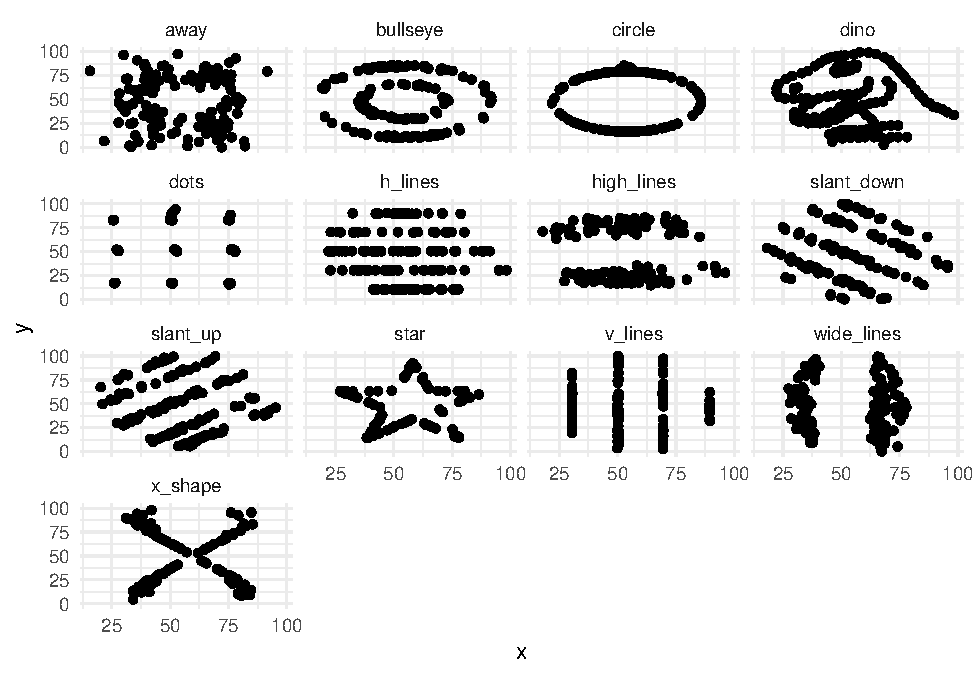
\includegraphics{ds-intro-till-r-bok_files/figure-latex/unnamed-chunk-26-1.pdf}

Eller som animering:

\begin{Shaded}
\begin{Highlighting}[]
\FunctionTok{library}\NormalTok{(datasauRus)}
\FunctionTok{library}\NormalTok{(ggplot2)}
\FunctionTok{library}\NormalTok{(gganimate)}

\FunctionTok{ggplot}\NormalTok{(datasaurus\_dozen, }\FunctionTok{aes}\NormalTok{(}\AttributeTok{x=}\NormalTok{x, }\AttributeTok{y=}\NormalTok{y))}\SpecialCharTok{+}
  \FunctionTok{geom\_point}\NormalTok{()}\SpecialCharTok{+}
  \FunctionTok{theme\_minimal}\NormalTok{() }\SpecialCharTok{+}
  \FunctionTok{transition\_states}\NormalTok{(dataset, }\DecValTok{3}\NormalTok{, }\DecValTok{1}\NormalTok{) }\SpecialCharTok{+} 
  \FunctionTok{ease\_aes}\NormalTok{(}\StringTok{\textquotesingle{}cubic{-}in{-}out\textquotesingle{}}\NormalTok{)}
\end{Highlighting}
\end{Shaded}

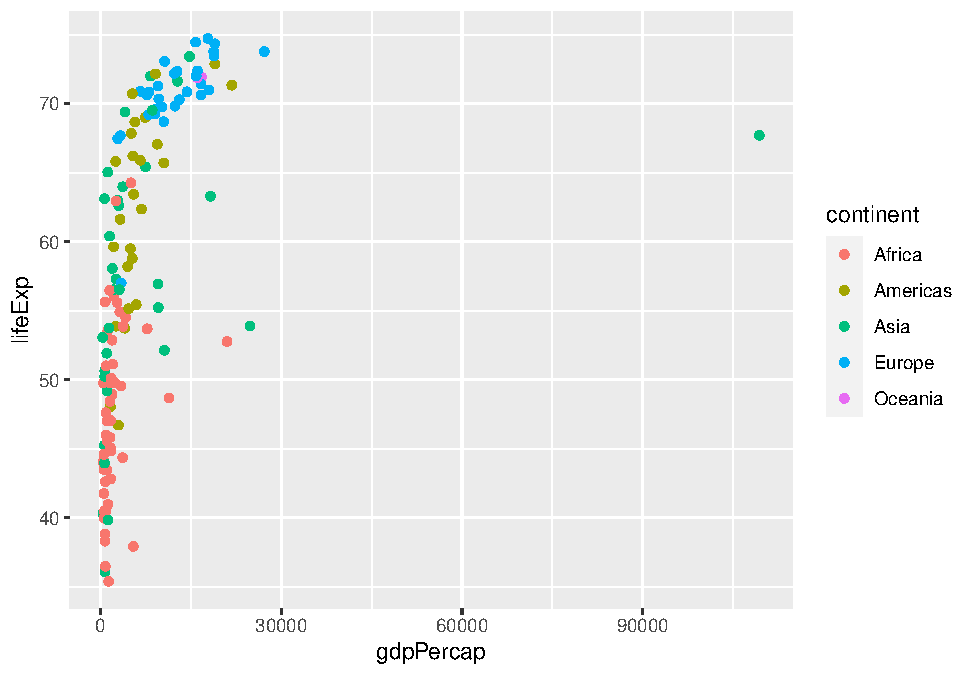
\includegraphics{ds-intro-till-r-bok_files/figure-latex/unnamed-chunk-27-1.pdf} 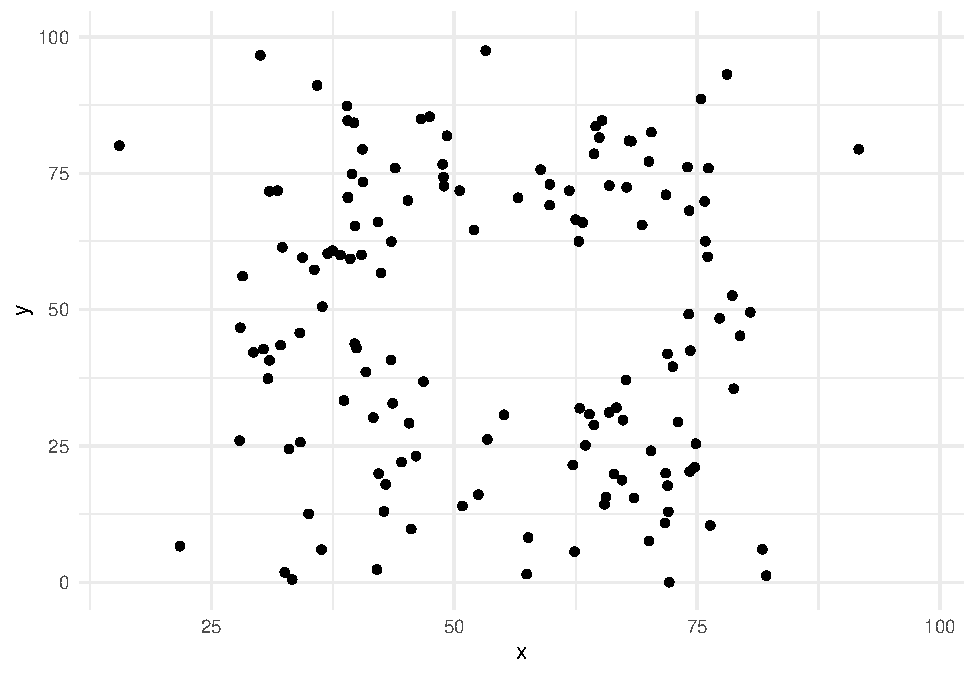
\includegraphics{ds-intro-till-r-bok_files/figure-latex/unnamed-chunk-27-2.pdf} 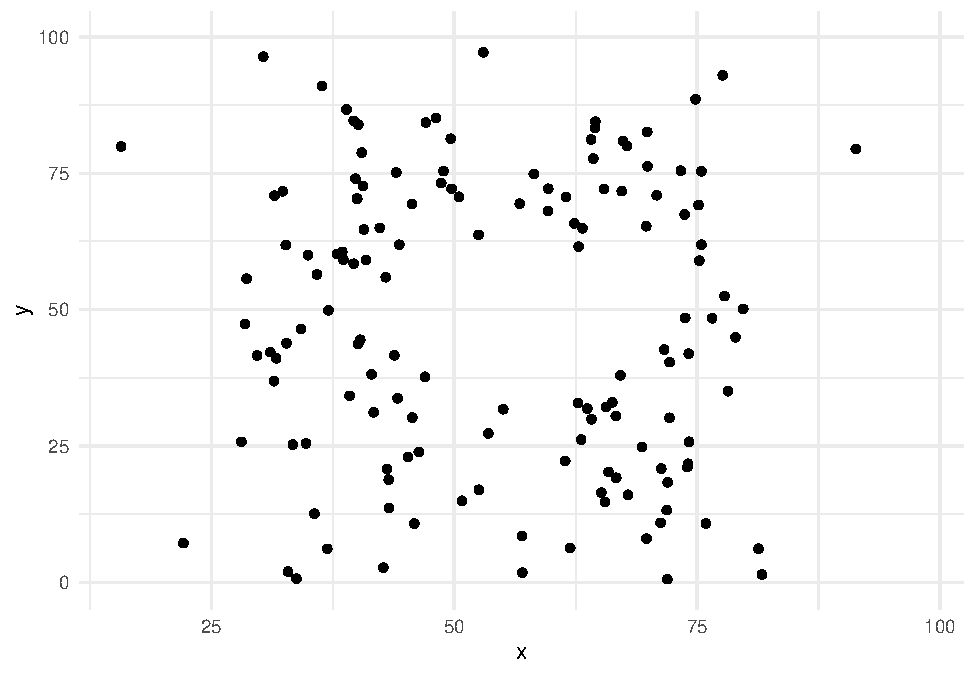
\includegraphics{ds-intro-till-r-bok_files/figure-latex/unnamed-chunk-27-3.pdf} 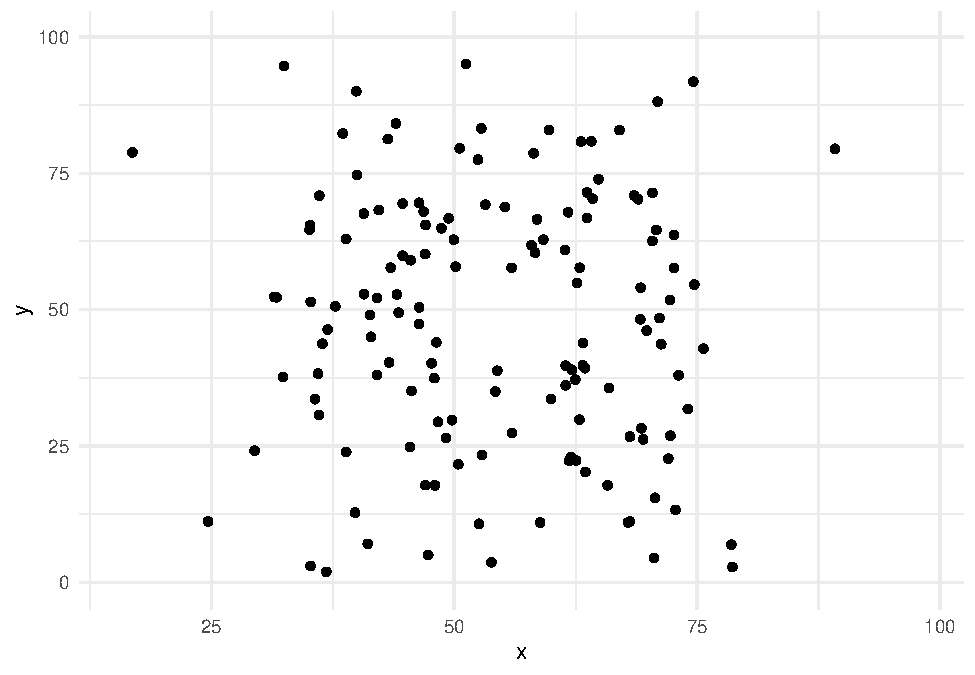
\includegraphics{ds-intro-till-r-bok_files/figure-latex/unnamed-chunk-27-4.pdf} 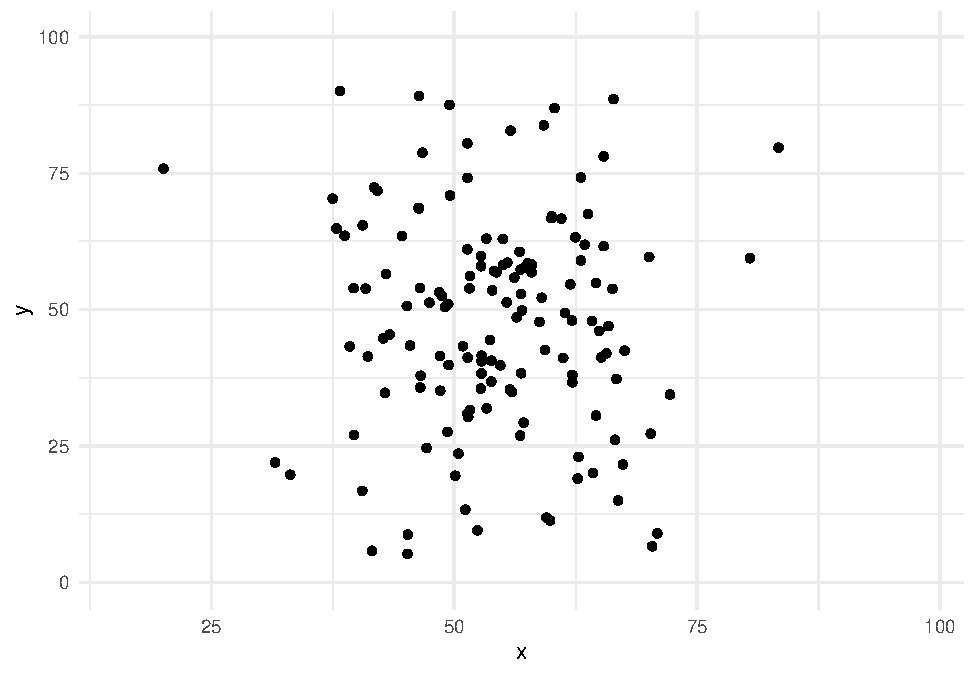
\includegraphics{ds-intro-till-r-bok_files/figure-latex/unnamed-chunk-27-5.pdf} 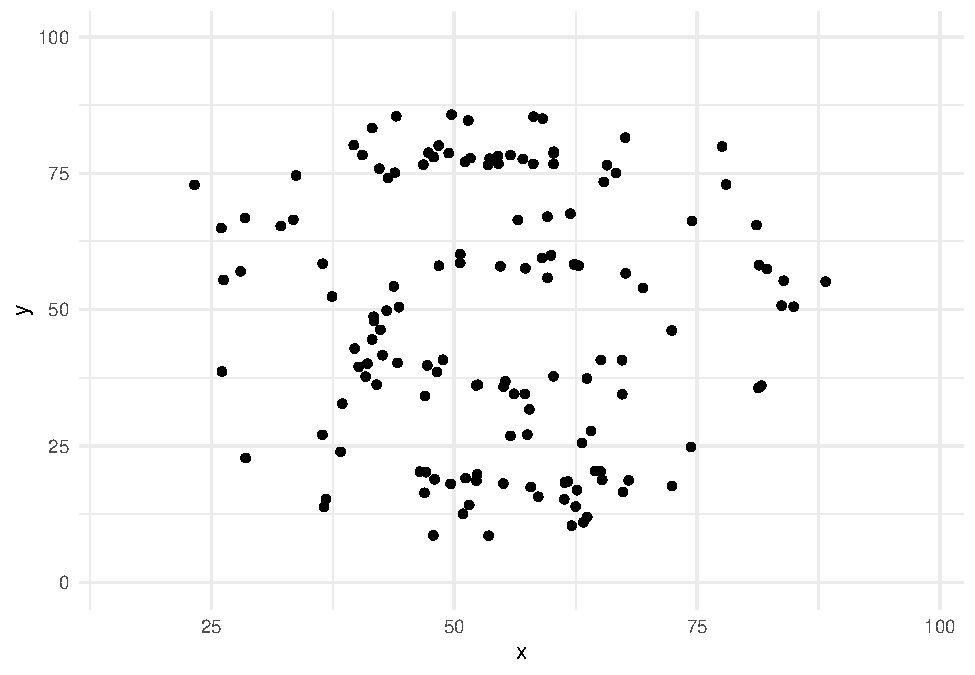
\includegraphics{ds-intro-till-r-bok_files/figure-latex/unnamed-chunk-27-6.pdf} 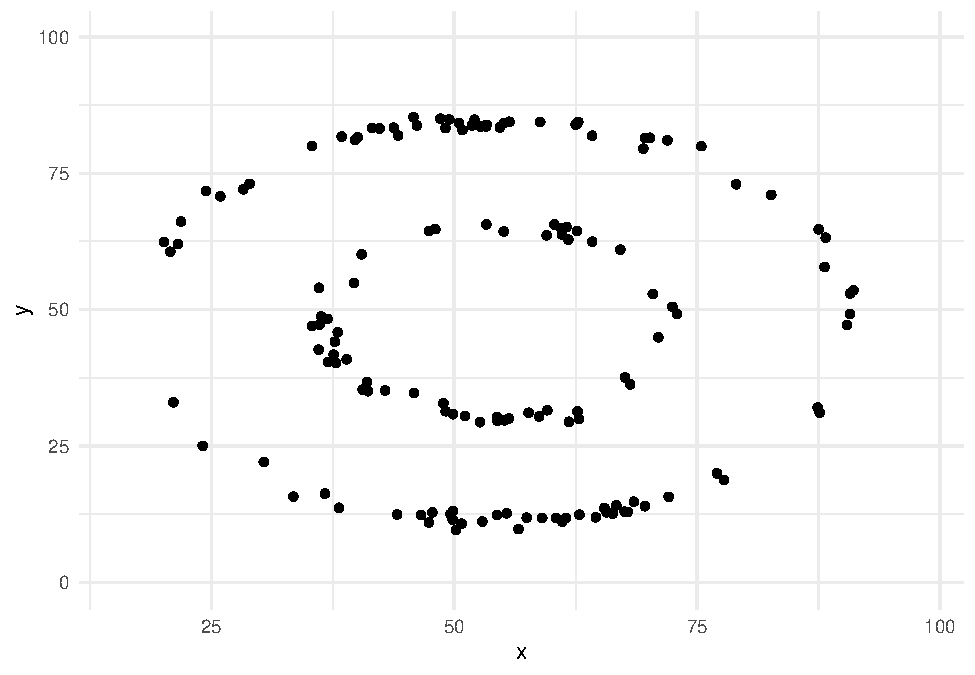
\includegraphics{ds-intro-till-r-bok_files/figure-latex/unnamed-chunk-27-7.pdf} 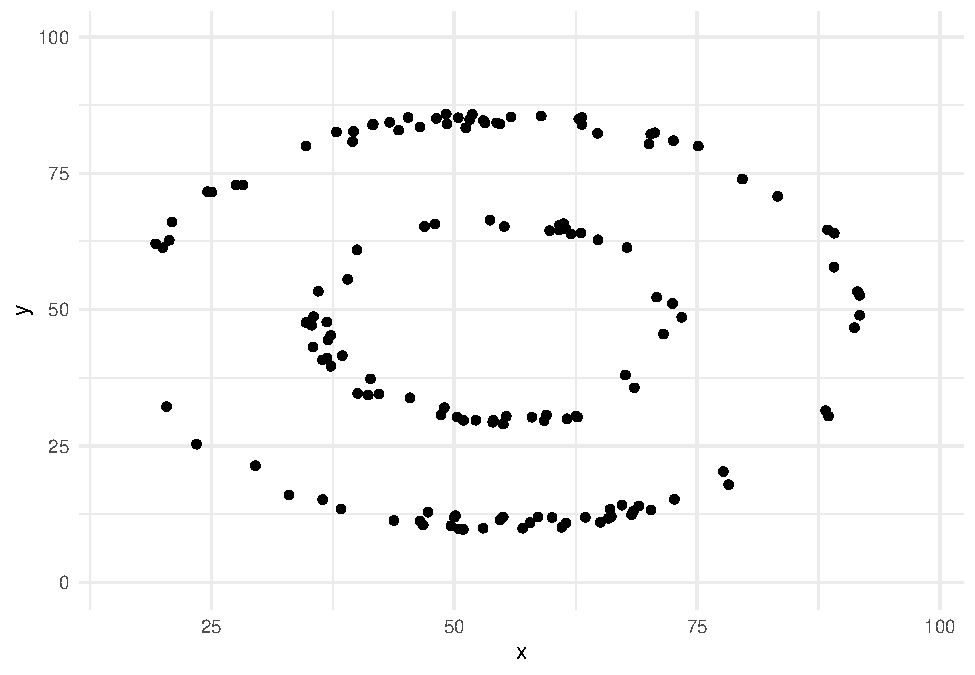
\includegraphics{ds-intro-till-r-bok_files/figure-latex/unnamed-chunk-27-8.pdf} 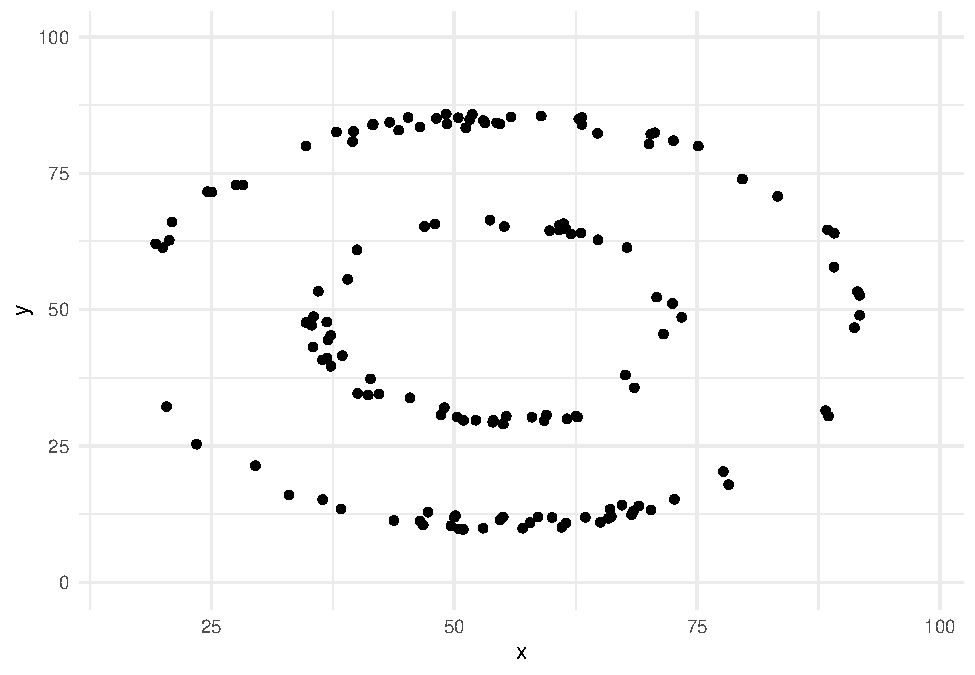
\includegraphics{ds-intro-till-r-bok_files/figure-latex/unnamed-chunk-27-9.pdf} 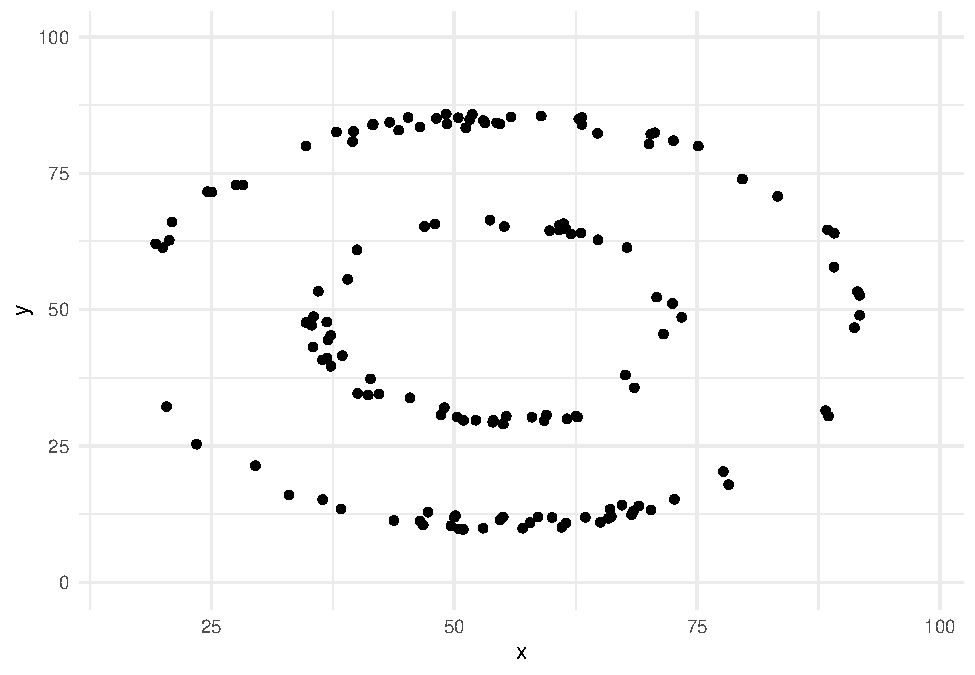
\includegraphics{ds-intro-till-r-bok_files/figure-latex/unnamed-chunk-27-10.pdf} 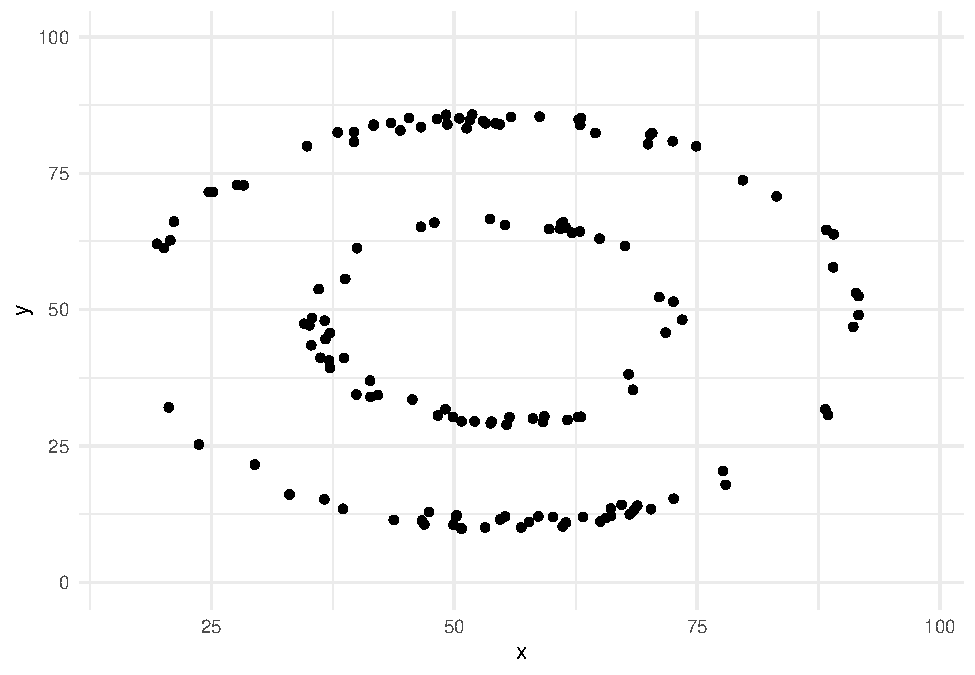
\includegraphics{ds-intro-till-r-bok_files/figure-latex/unnamed-chunk-27-11.pdf} 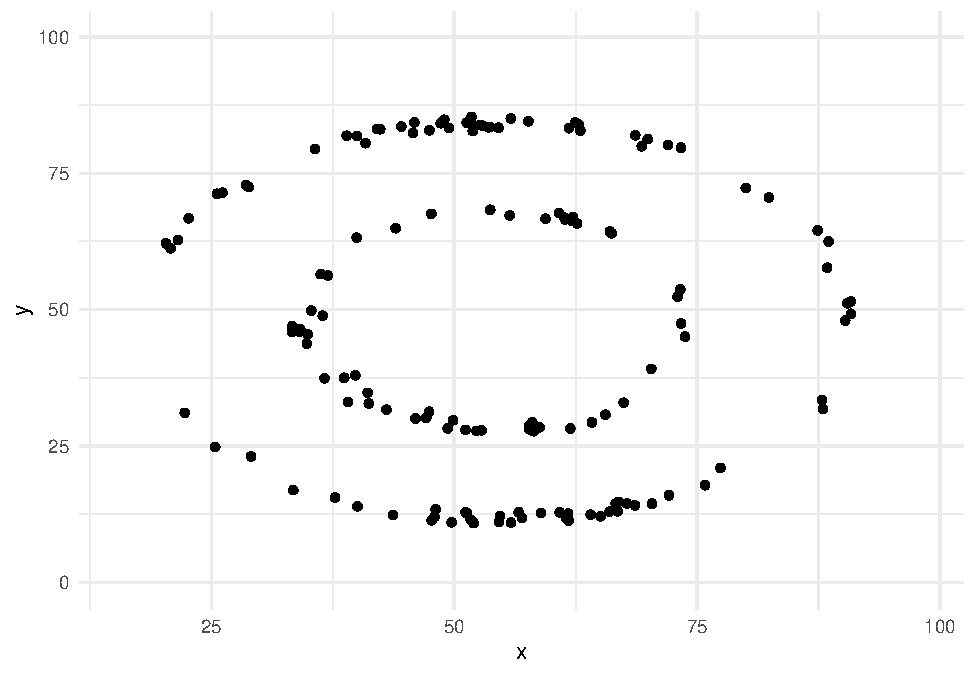
\includegraphics{ds-intro-till-r-bok_files/figure-latex/unnamed-chunk-27-12.pdf} 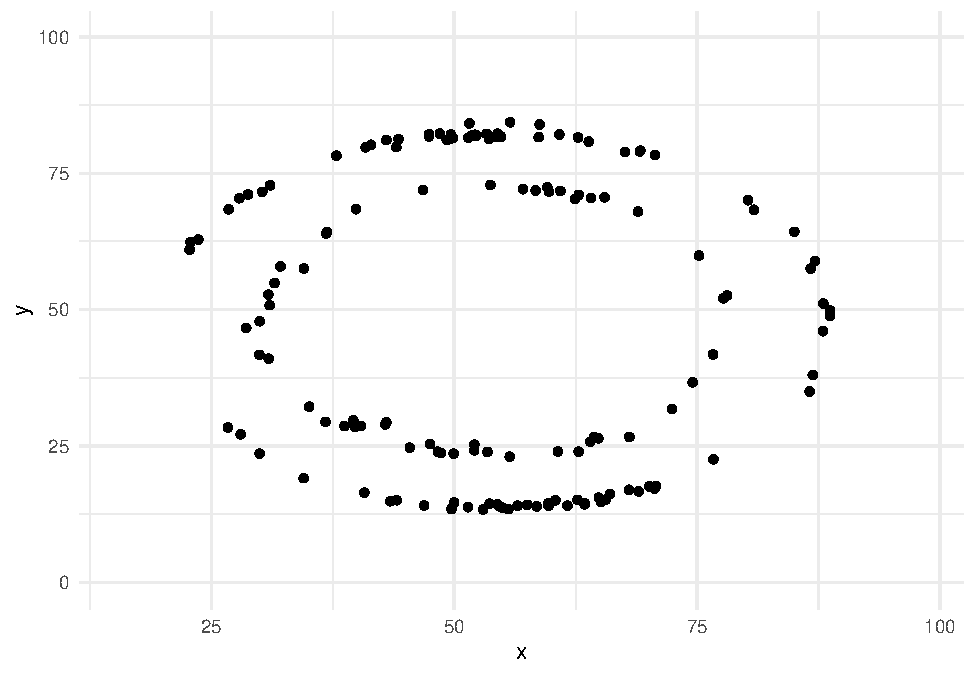
\includegraphics{ds-intro-till-r-bok_files/figure-latex/unnamed-chunk-27-13.pdf} 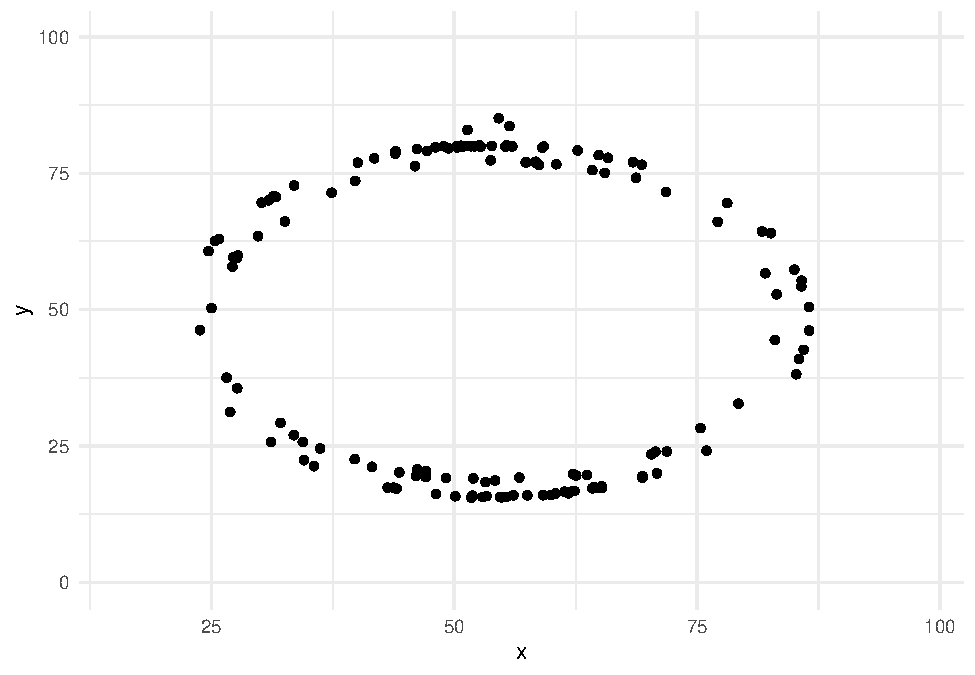
\includegraphics{ds-intro-till-r-bok_files/figure-latex/unnamed-chunk-27-14.pdf} 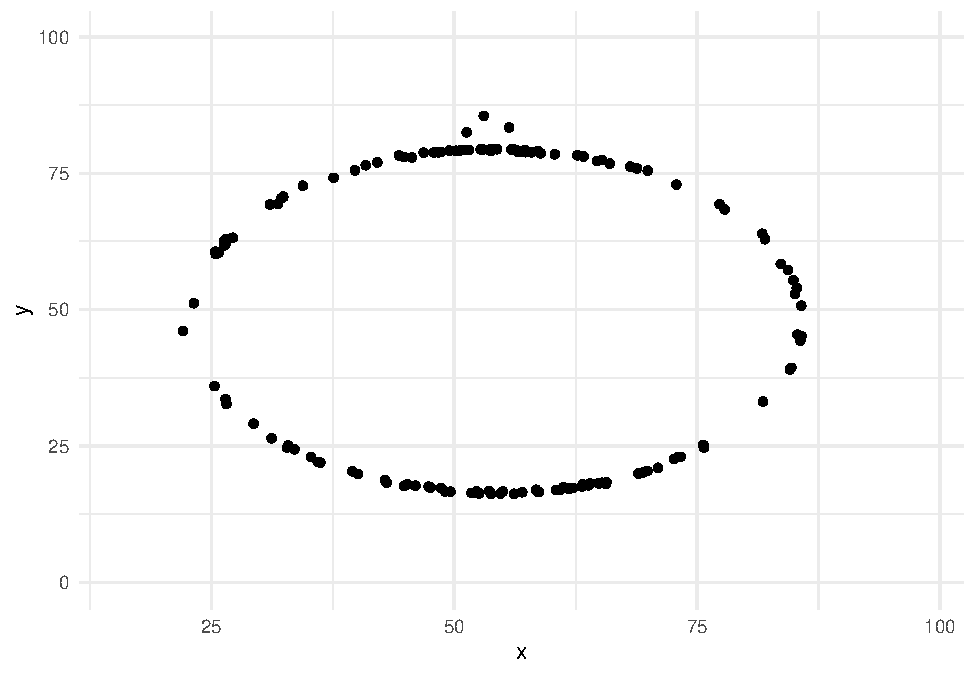
\includegraphics{ds-intro-till-r-bok_files/figure-latex/unnamed-chunk-27-15.pdf} 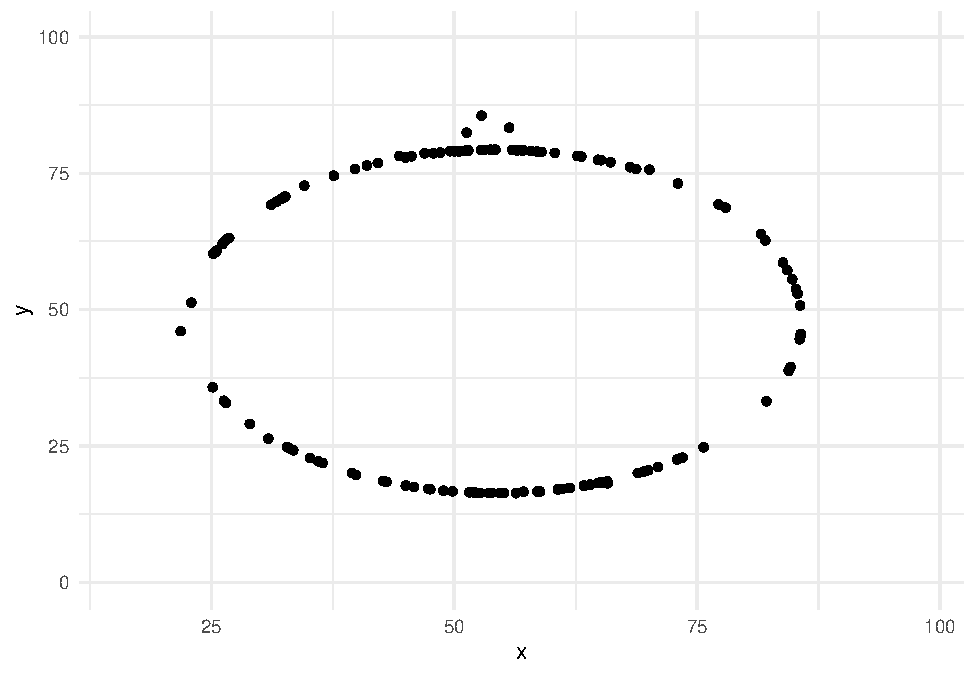
\includegraphics{ds-intro-till-r-bok_files/figure-latex/unnamed-chunk-27-16.pdf} 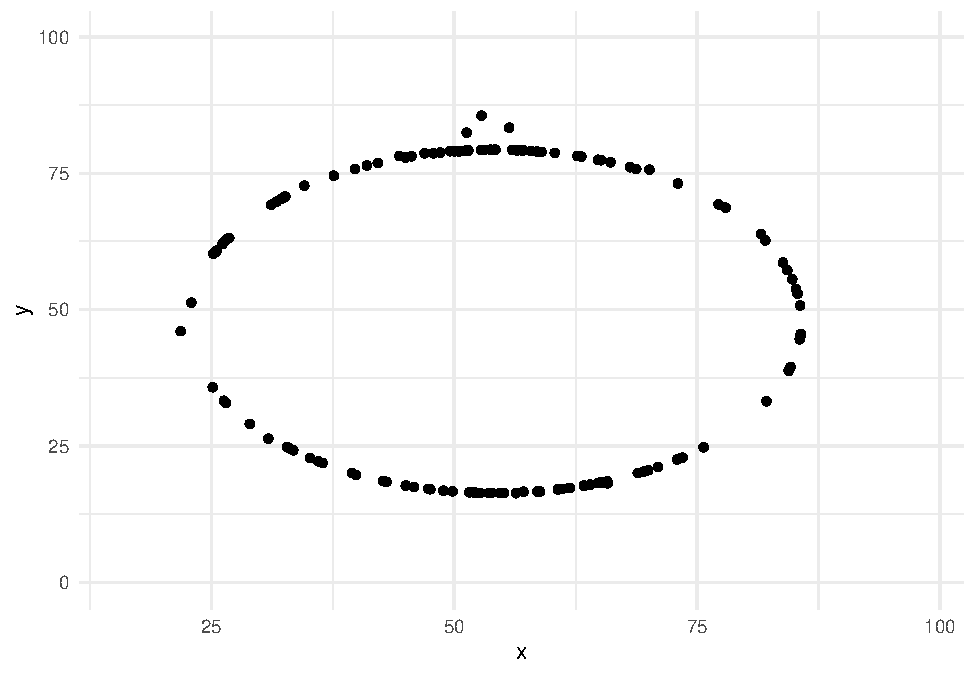
\includegraphics{ds-intro-till-r-bok_files/figure-latex/unnamed-chunk-27-17.pdf} 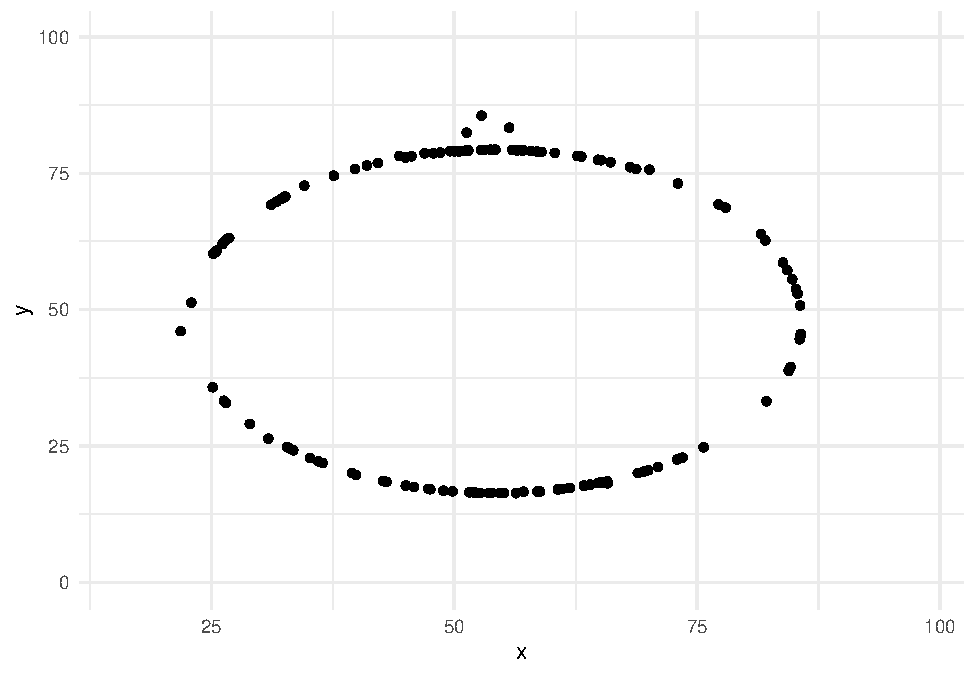
\includegraphics{ds-intro-till-r-bok_files/figure-latex/unnamed-chunk-27-18.pdf} 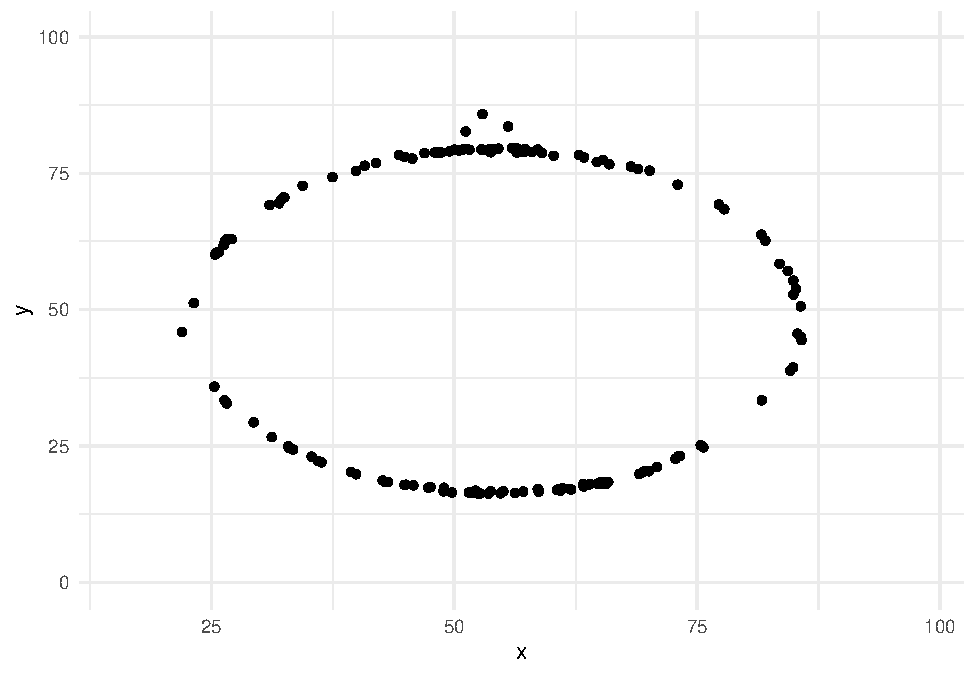
\includegraphics{ds-intro-till-r-bok_files/figure-latex/unnamed-chunk-27-19.pdf} 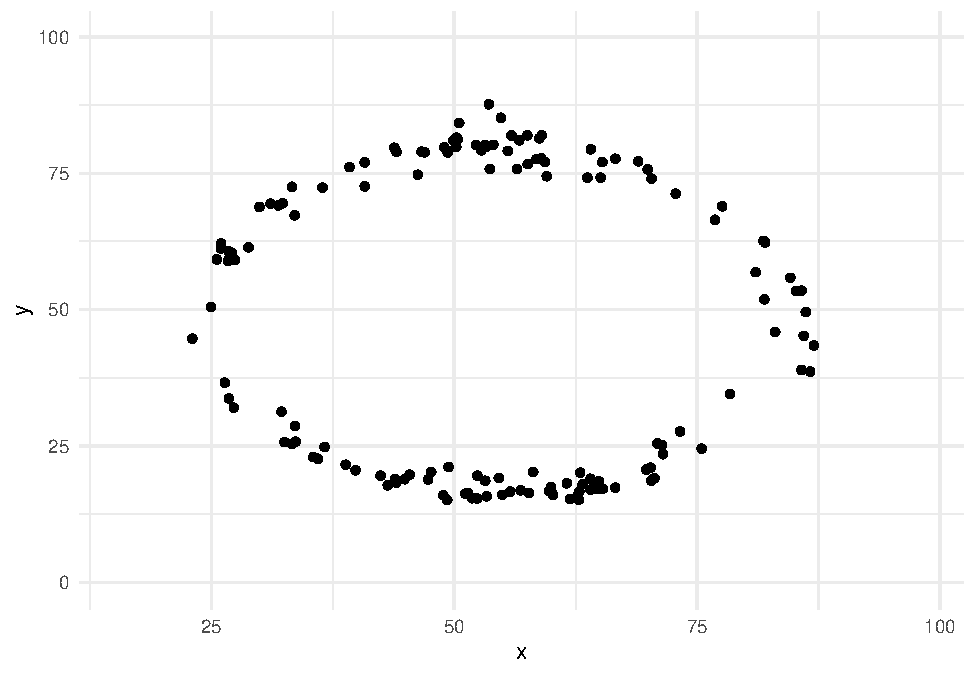
\includegraphics{ds-intro-till-r-bok_files/figure-latex/unnamed-chunk-27-20.pdf} 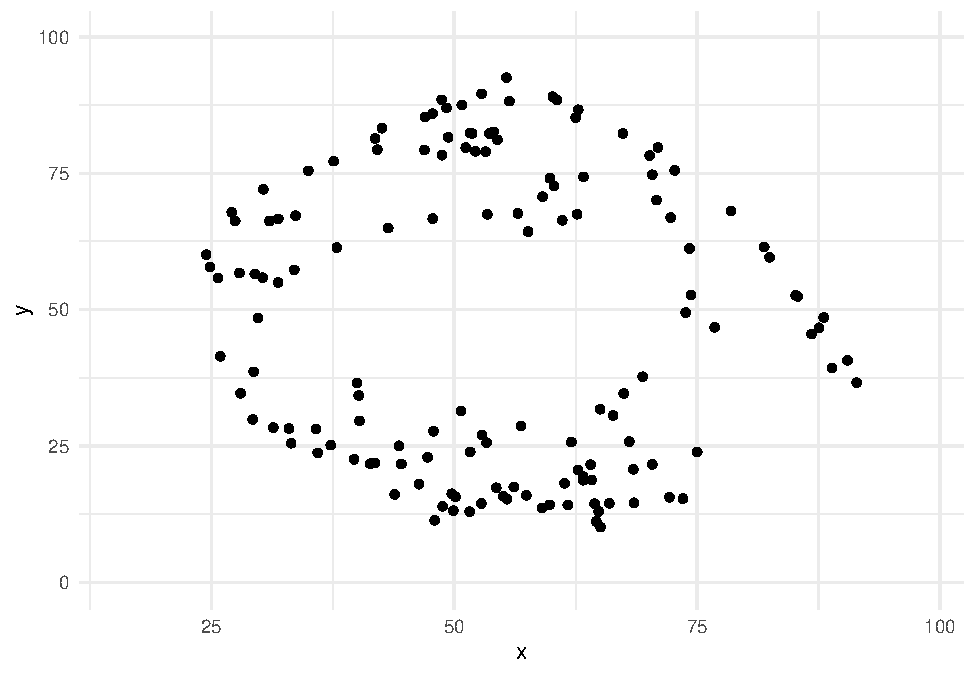
\includegraphics{ds-intro-till-r-bok_files/figure-latex/unnamed-chunk-27-21.pdf} 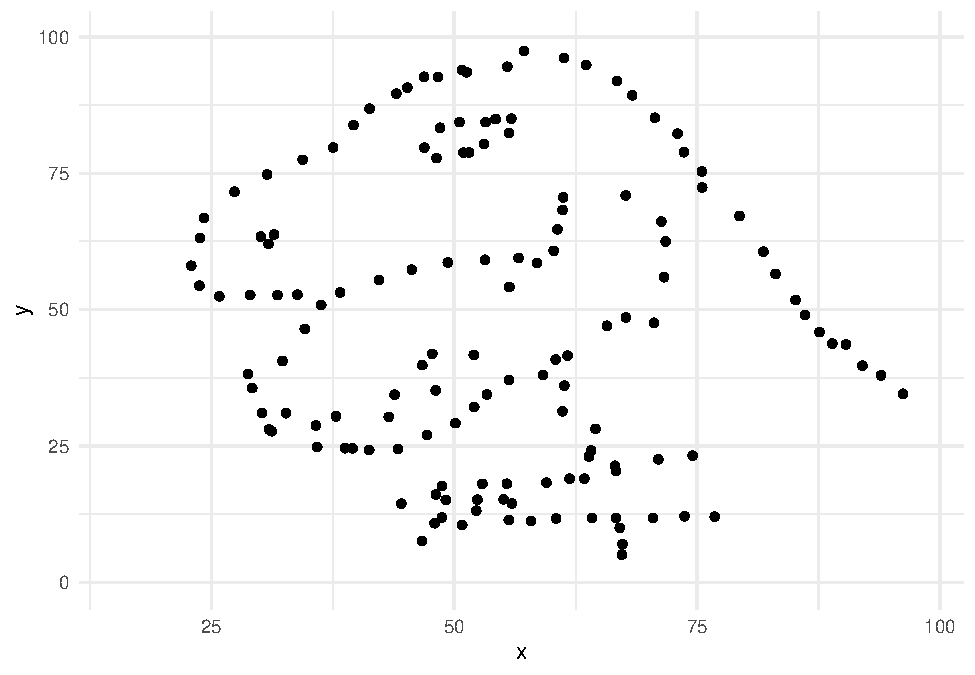
\includegraphics{ds-intro-till-r-bok_files/figure-latex/unnamed-chunk-27-22.pdf} 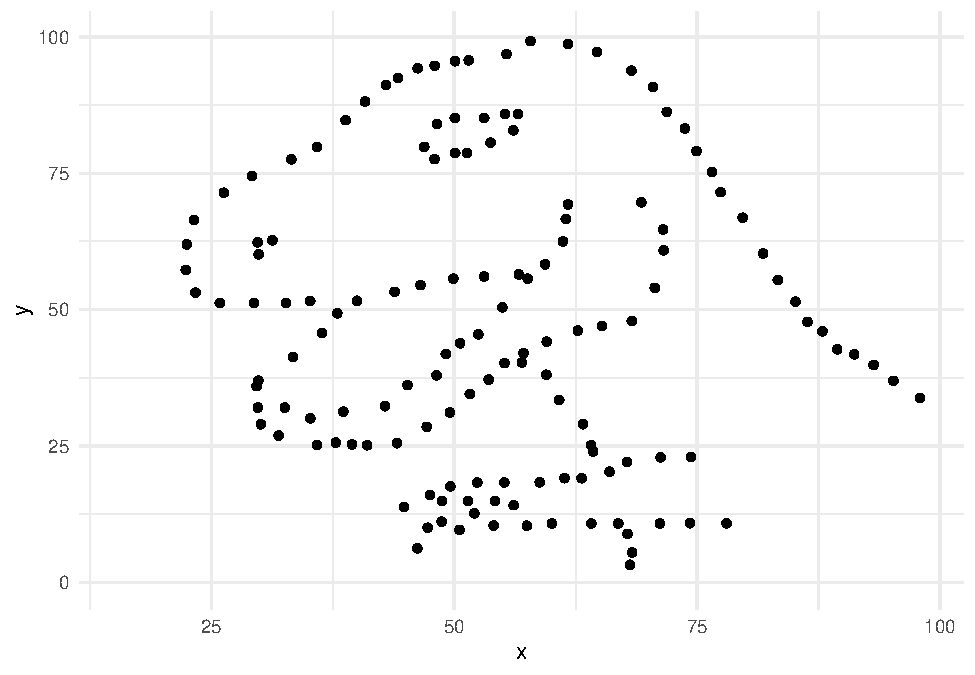
\includegraphics{ds-intro-till-r-bok_files/figure-latex/unnamed-chunk-27-23.pdf} 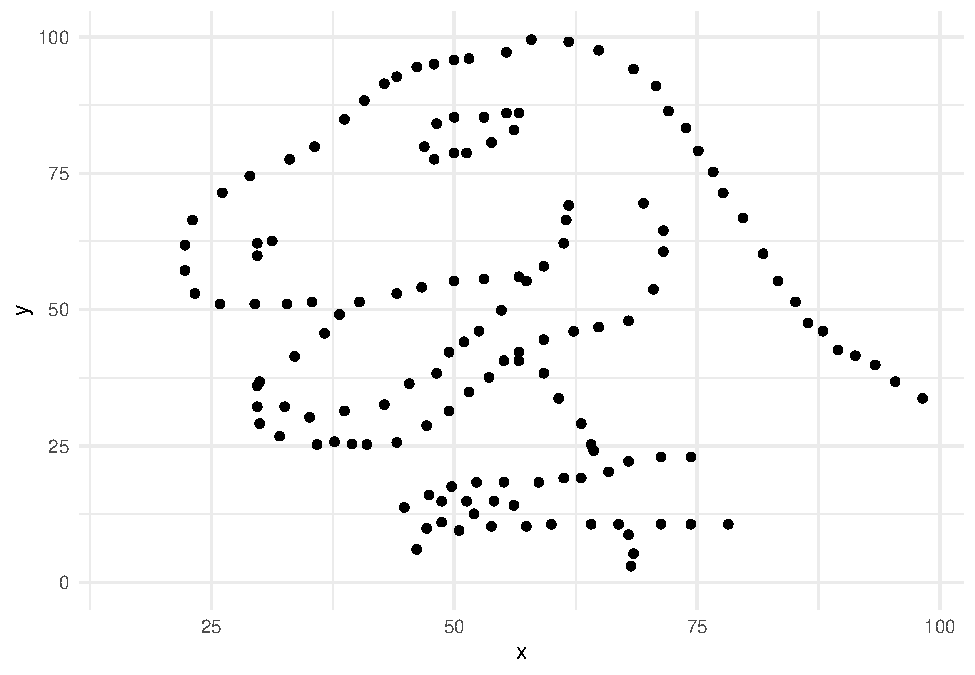
\includegraphics{ds-intro-till-r-bok_files/figure-latex/unnamed-chunk-27-24.pdf} 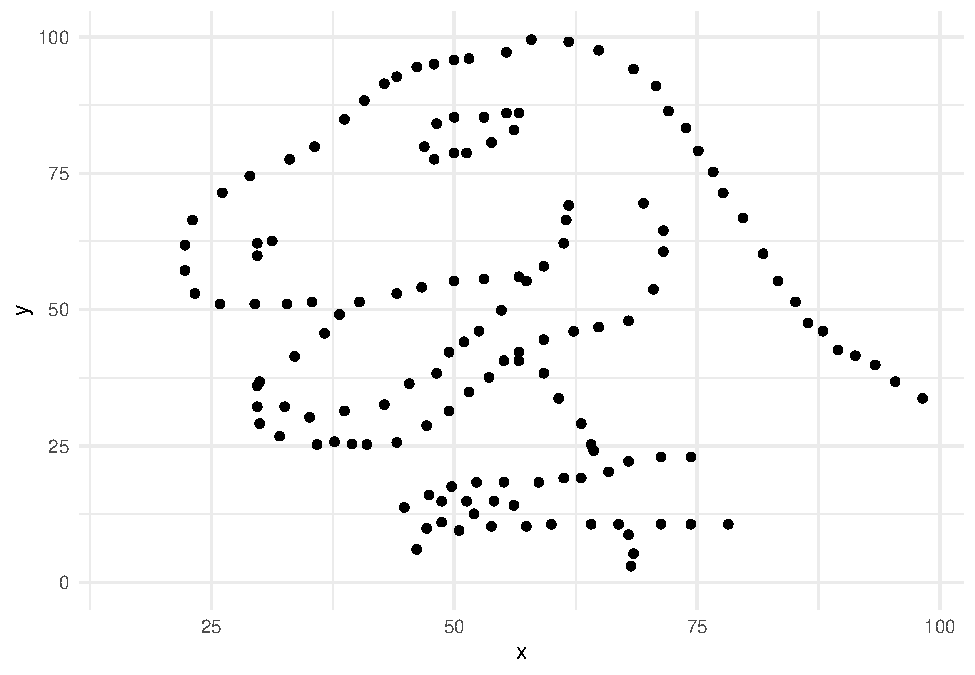
\includegraphics{ds-intro-till-r-bok_files/figure-latex/unnamed-chunk-27-25.pdf} 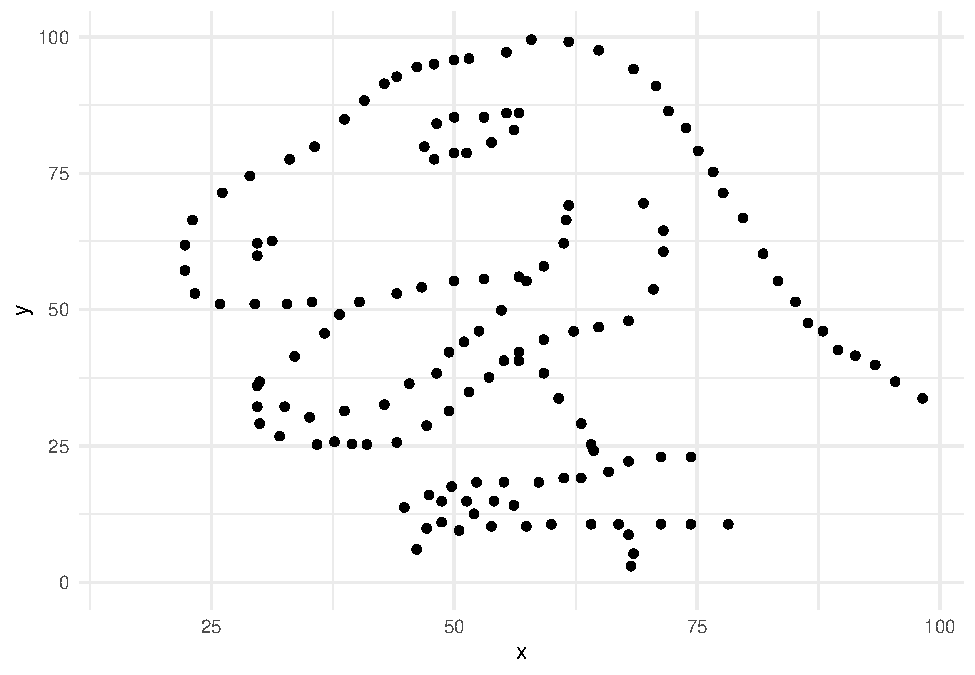
\includegraphics{ds-intro-till-r-bok_files/figure-latex/unnamed-chunk-27-26.pdf} 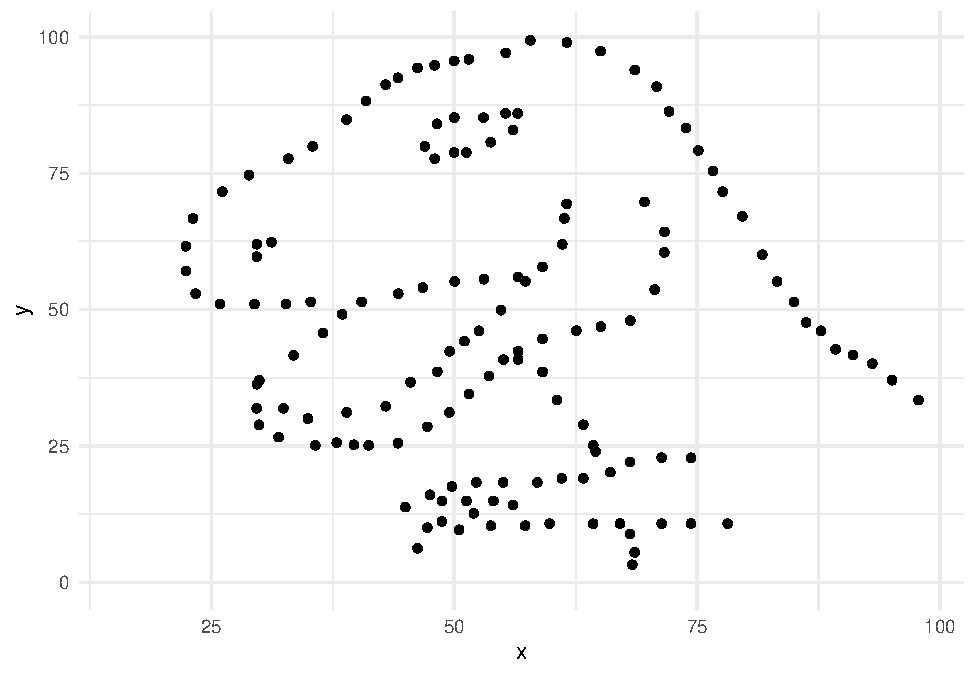
\includegraphics{ds-intro-till-r-bok_files/figure-latex/unnamed-chunk-27-27.pdf} 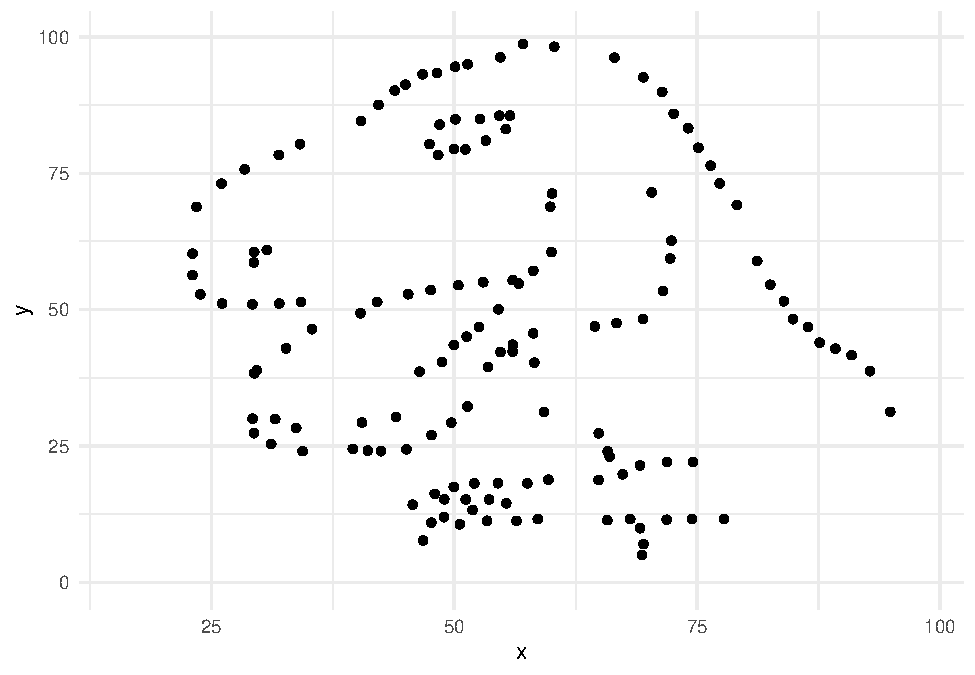
\includegraphics{ds-intro-till-r-bok_files/figure-latex/unnamed-chunk-27-28.pdf} 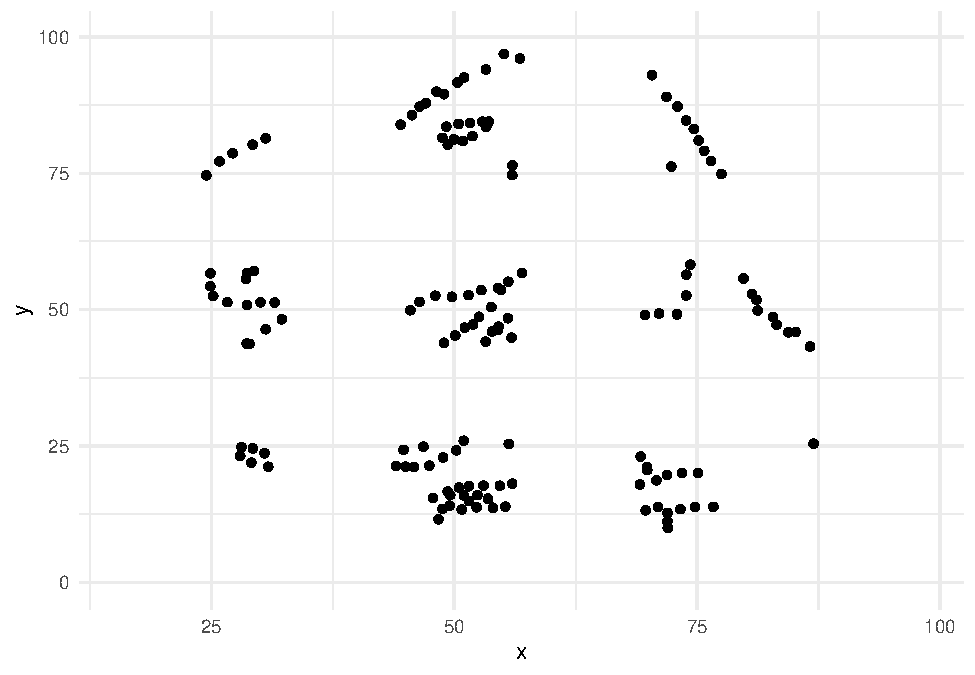
\includegraphics{ds-intro-till-r-bok_files/figure-latex/unnamed-chunk-27-29.pdf} 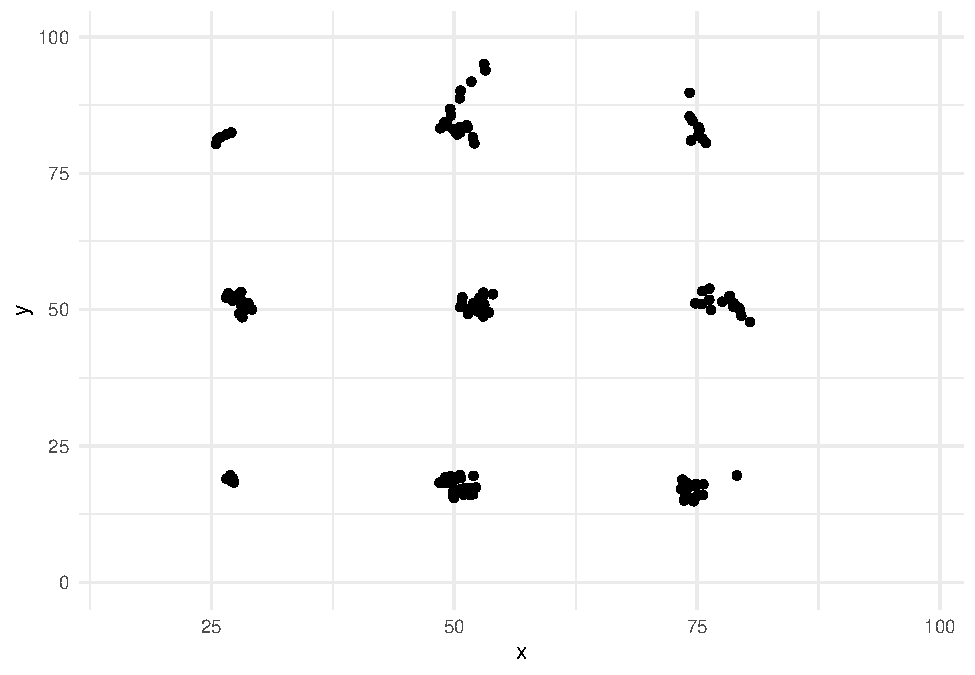
\includegraphics{ds-intro-till-r-bok_files/figure-latex/unnamed-chunk-27-30.pdf} 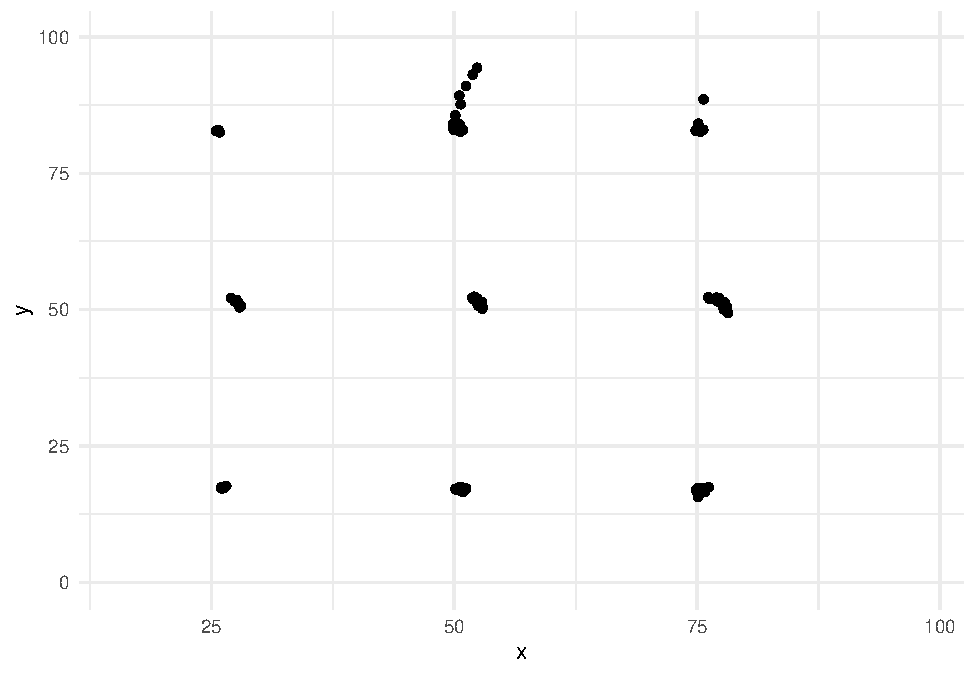
\includegraphics{ds-intro-till-r-bok_files/figure-latex/unnamed-chunk-27-31.pdf} 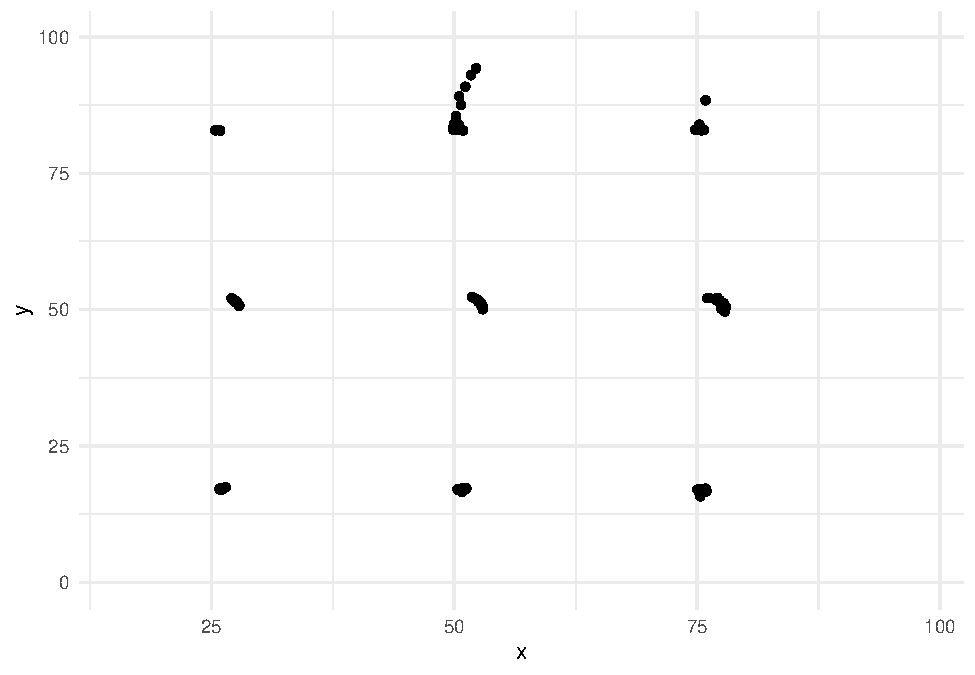
\includegraphics{ds-intro-till-r-bok_files/figure-latex/unnamed-chunk-27-32.pdf} 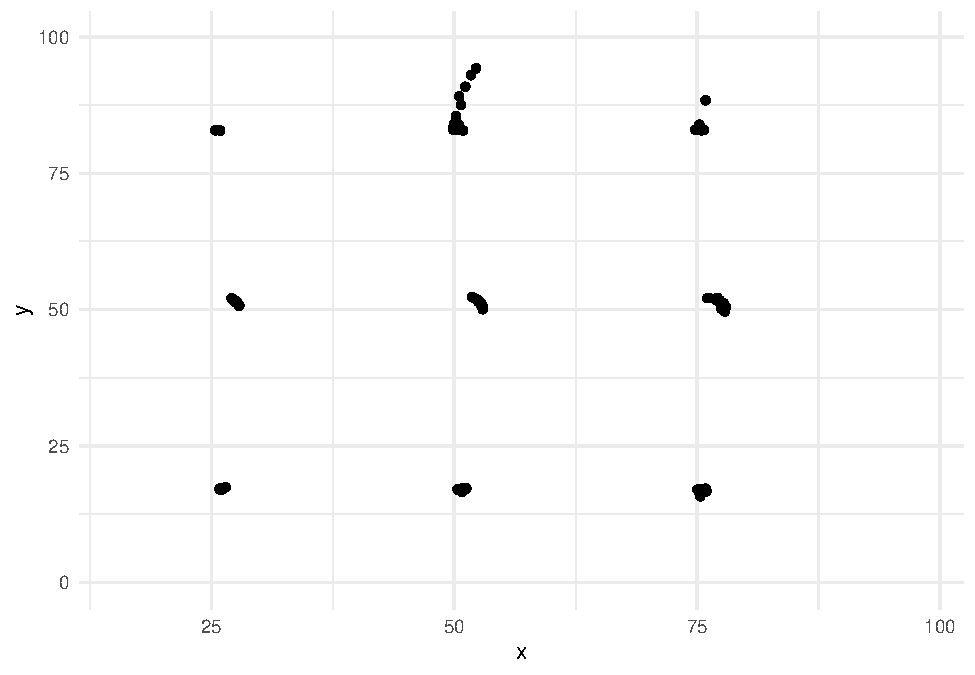
\includegraphics{ds-intro-till-r-bok_files/figure-latex/unnamed-chunk-27-33.pdf} 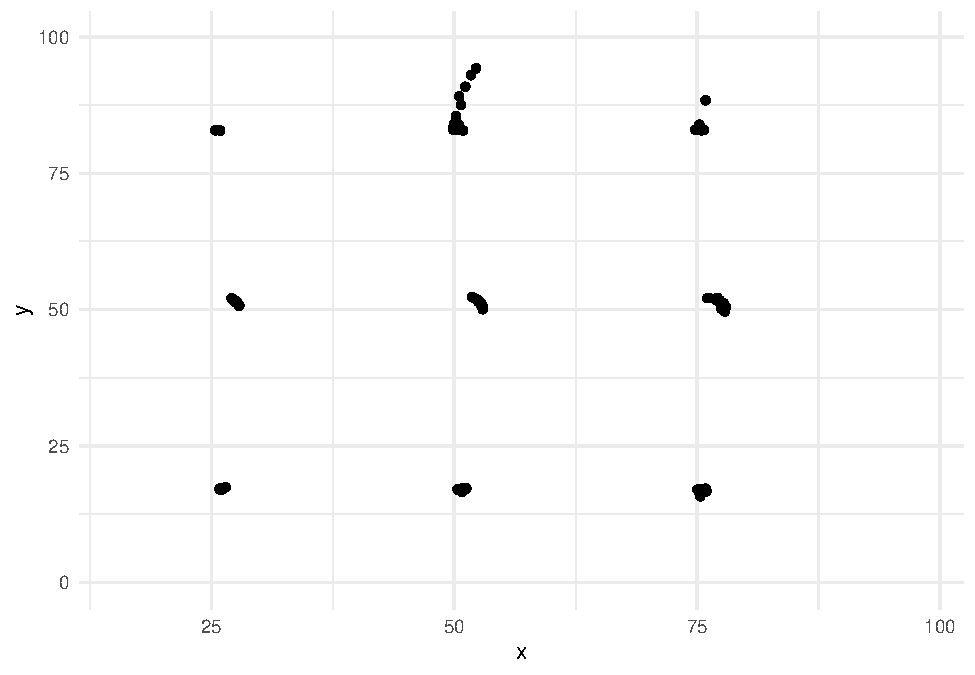
\includegraphics{ds-intro-till-r-bok_files/figure-latex/unnamed-chunk-27-34.pdf} 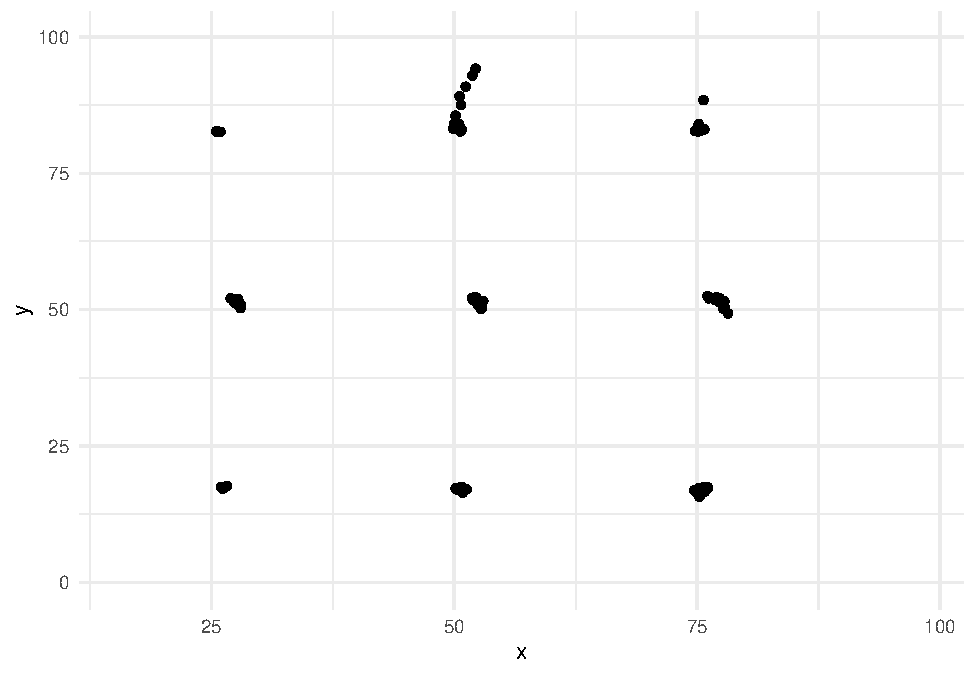
\includegraphics{ds-intro-till-r-bok_files/figure-latex/unnamed-chunk-27-35.pdf} 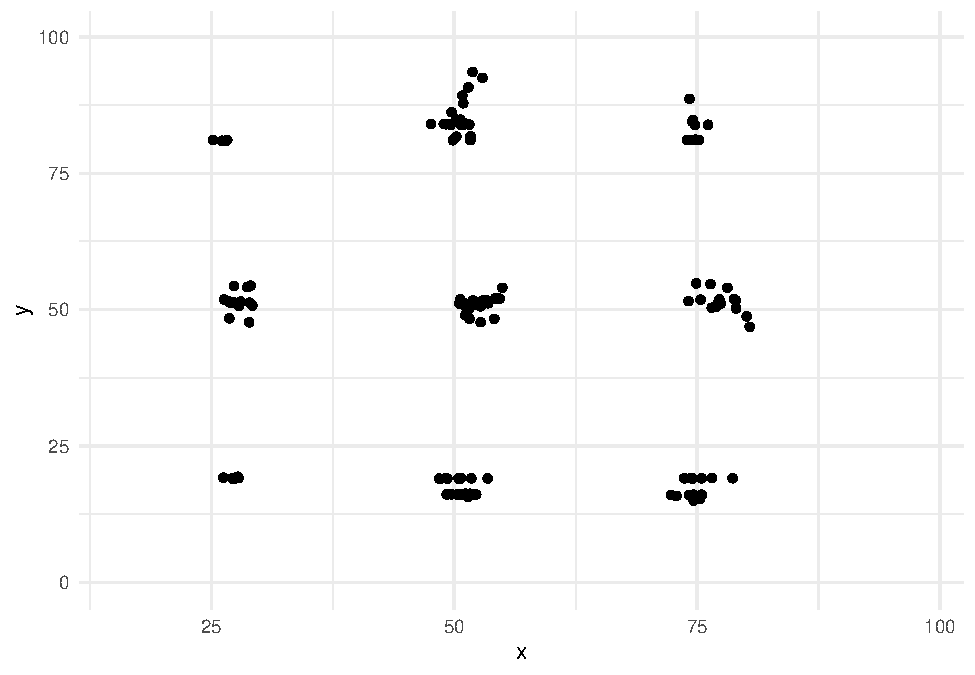
\includegraphics{ds-intro-till-r-bok_files/figure-latex/unnamed-chunk-27-36.pdf} 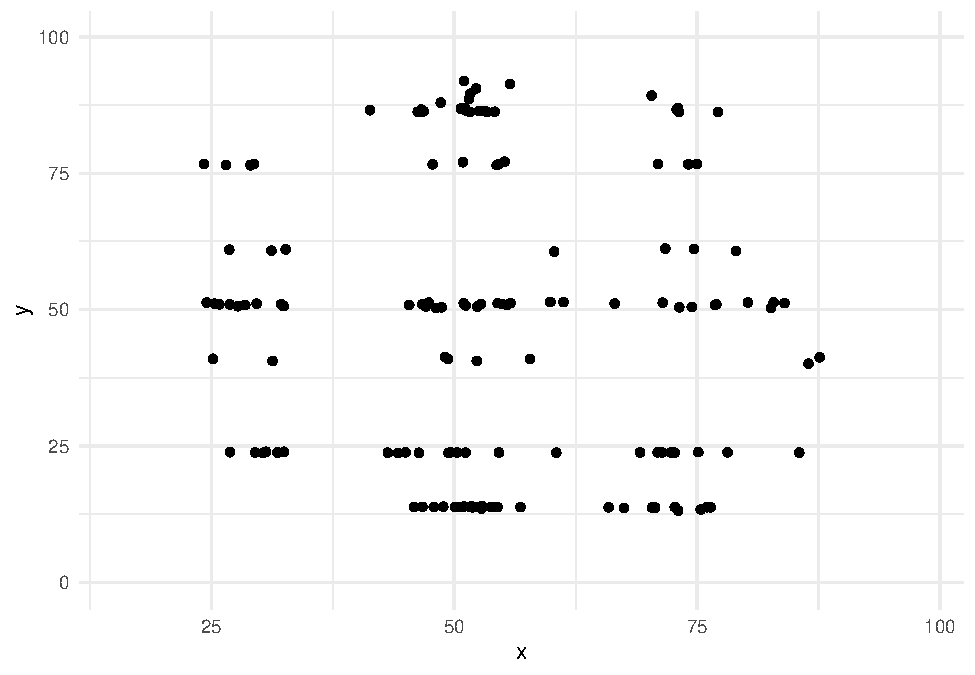
\includegraphics{ds-intro-till-r-bok_files/figure-latex/unnamed-chunk-27-37.pdf} 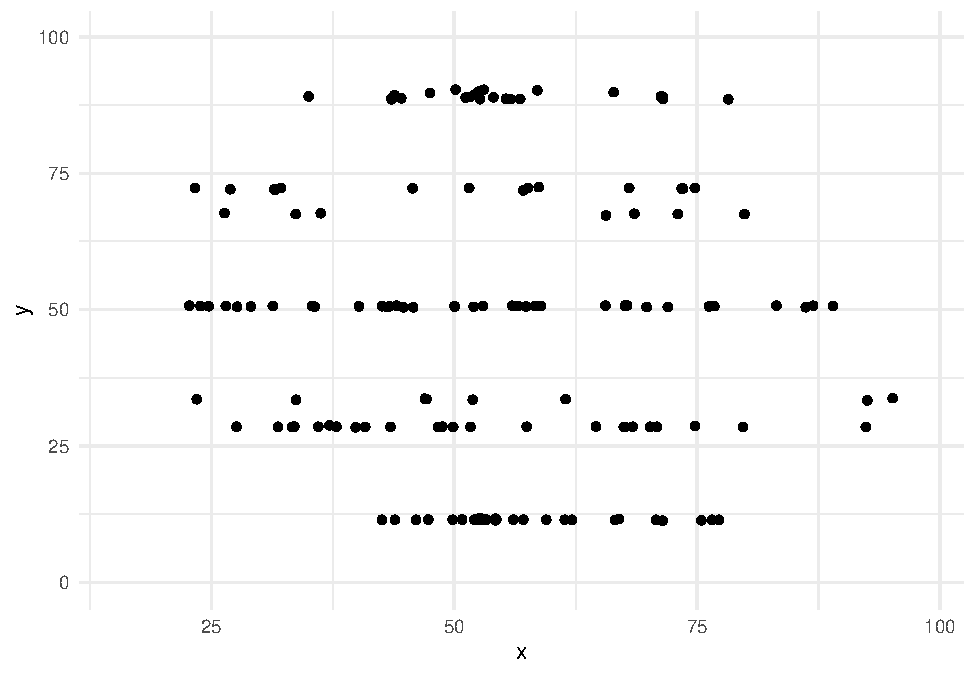
\includegraphics{ds-intro-till-r-bok_files/figure-latex/unnamed-chunk-27-38.pdf} 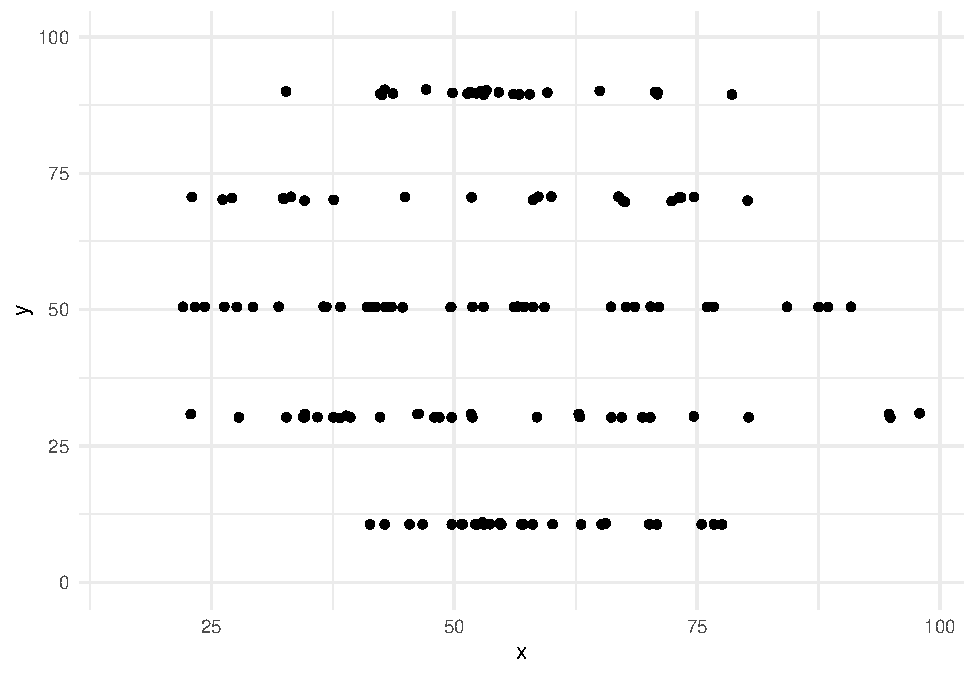
\includegraphics{ds-intro-till-r-bok_files/figure-latex/unnamed-chunk-27-39.pdf} 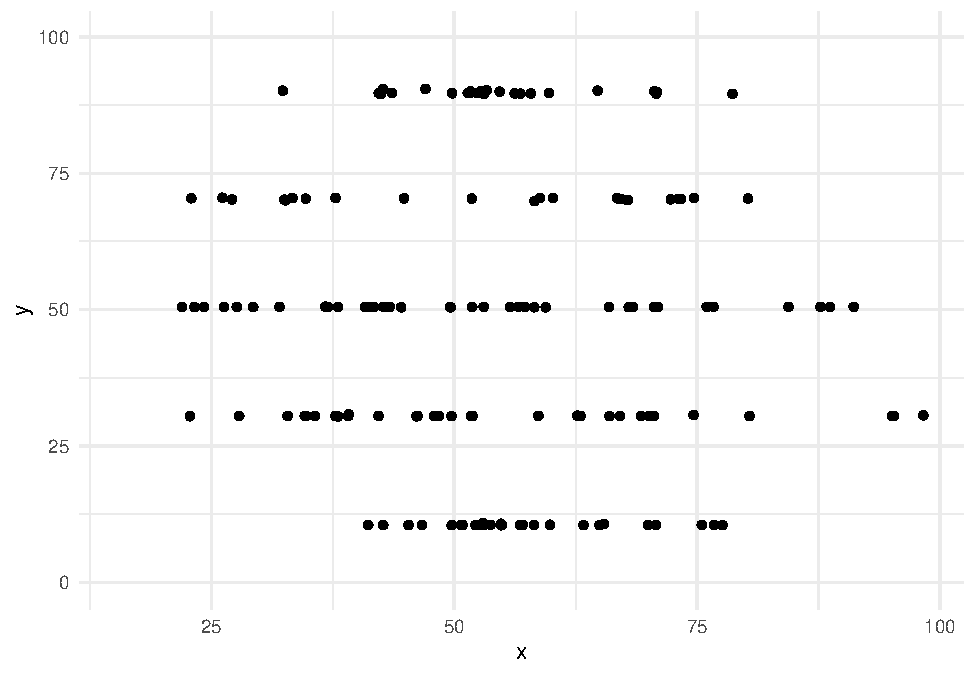
\includegraphics{ds-intro-till-r-bok_files/figure-latex/unnamed-chunk-27-40.pdf} 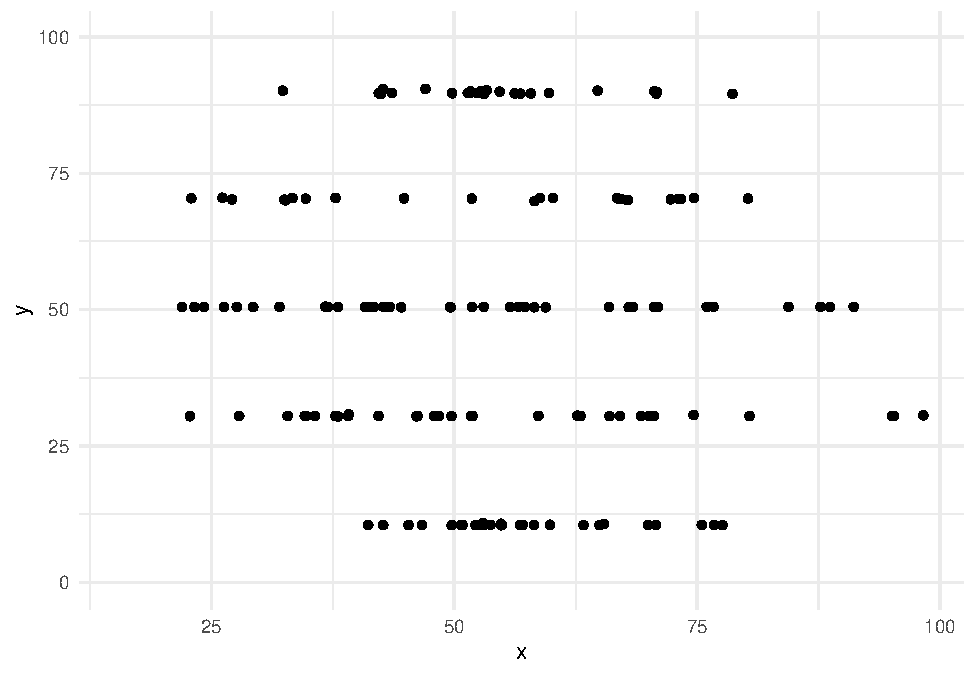
\includegraphics{ds-intro-till-r-bok_files/figure-latex/unnamed-chunk-27-41.pdf} 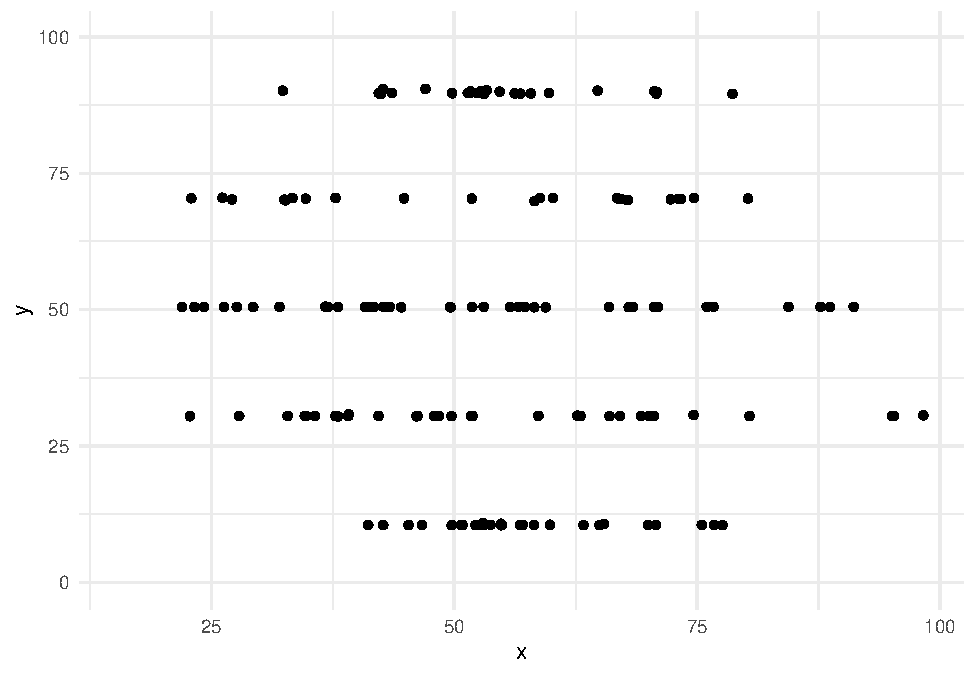
\includegraphics{ds-intro-till-r-bok_files/figure-latex/unnamed-chunk-27-42.pdf} 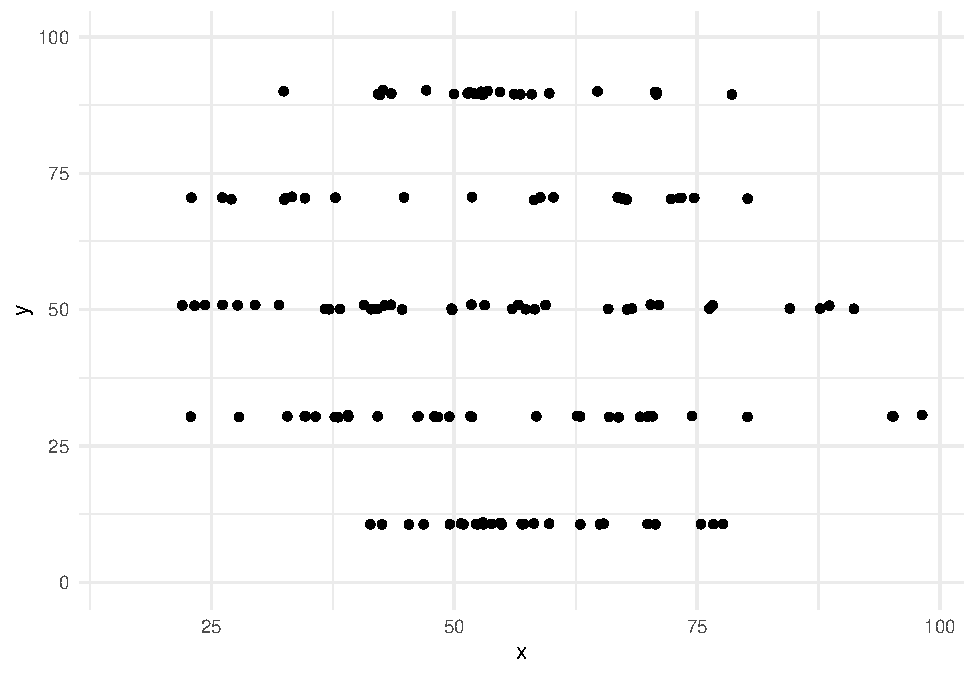
\includegraphics{ds-intro-till-r-bok_files/figure-latex/unnamed-chunk-27-43.pdf} 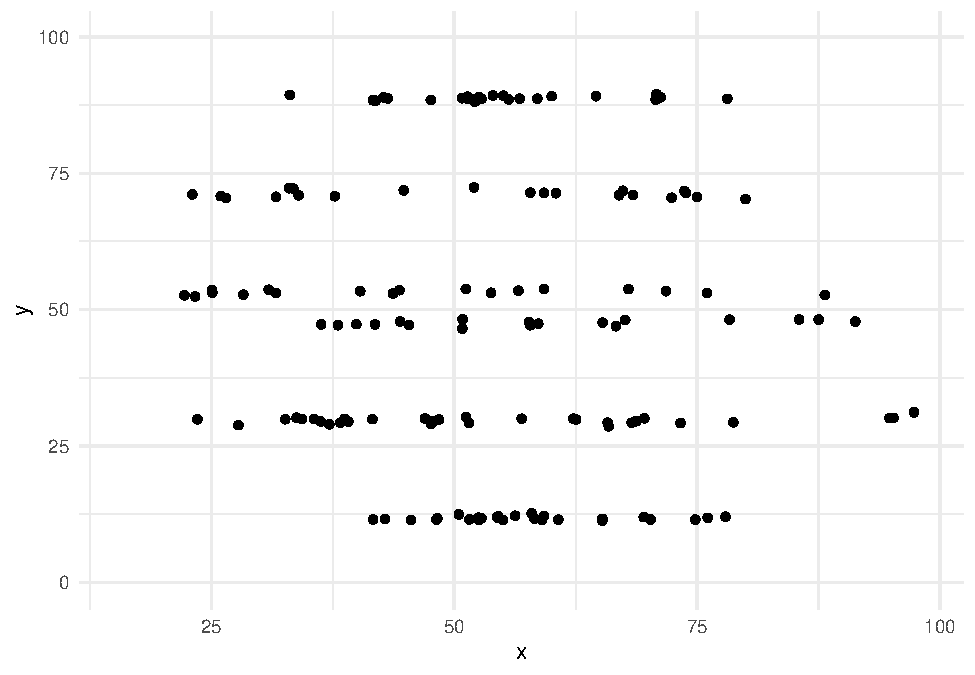
\includegraphics{ds-intro-till-r-bok_files/figure-latex/unnamed-chunk-27-44.pdf} 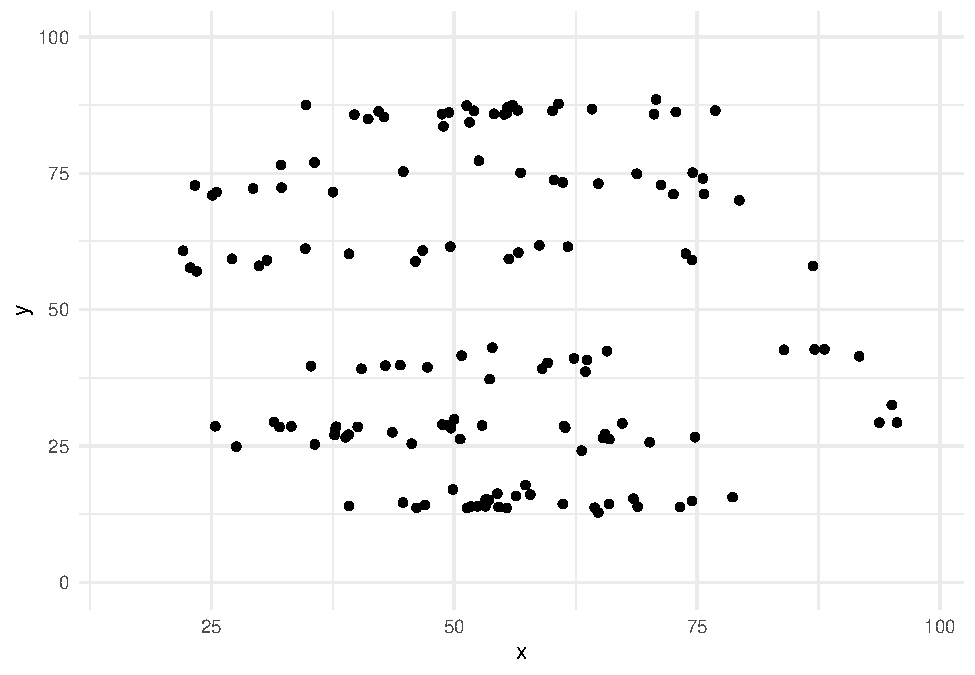
\includegraphics{ds-intro-till-r-bok_files/figure-latex/unnamed-chunk-27-45.pdf} 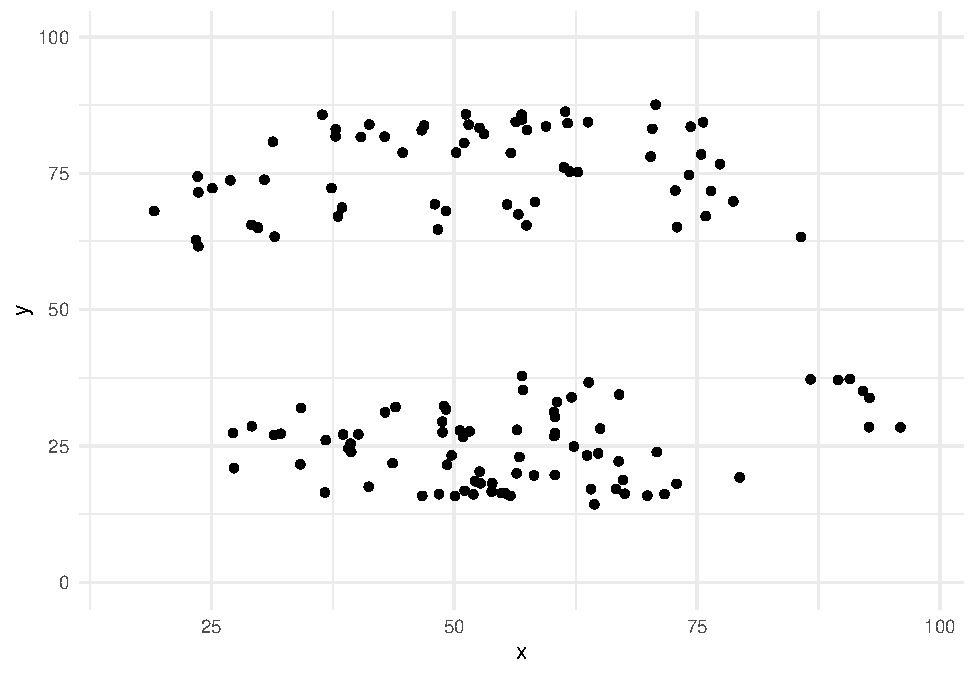
\includegraphics{ds-intro-till-r-bok_files/figure-latex/unnamed-chunk-27-46.pdf} \includegraphics{ds-intro-till-r-bok_files/figure-latex/unnamed-chunk-27-47.pdf} \includegraphics{ds-intro-till-r-bok_files/figure-latex/unnamed-chunk-27-48.pdf} \includegraphics{ds-intro-till-r-bok_files/figure-latex/unnamed-chunk-27-49.pdf} \includegraphics{ds-intro-till-r-bok_files/figure-latex/unnamed-chunk-27-50.pdf} \includegraphics{ds-intro-till-r-bok_files/figure-latex/unnamed-chunk-27-51.pdf} \includegraphics{ds-intro-till-r-bok_files/figure-latex/unnamed-chunk-27-52.pdf} \includegraphics{ds-intro-till-r-bok_files/figure-latex/unnamed-chunk-27-53.pdf} \includegraphics{ds-intro-till-r-bok_files/figure-latex/unnamed-chunk-27-54.pdf} \includegraphics{ds-intro-till-r-bok_files/figure-latex/unnamed-chunk-27-55.pdf} \includegraphics{ds-intro-till-r-bok_files/figure-latex/unnamed-chunk-27-56.pdf} \includegraphics{ds-intro-till-r-bok_files/figure-latex/unnamed-chunk-27-57.pdf} \includegraphics{ds-intro-till-r-bok_files/figure-latex/unnamed-chunk-27-58.pdf} \includegraphics{ds-intro-till-r-bok_files/figure-latex/unnamed-chunk-27-59.pdf} \includegraphics{ds-intro-till-r-bok_files/figure-latex/unnamed-chunk-27-60.pdf} \includegraphics{ds-intro-till-r-bok_files/figure-latex/unnamed-chunk-27-61.pdf} \includegraphics{ds-intro-till-r-bok_files/figure-latex/unnamed-chunk-27-62.pdf} \includegraphics{ds-intro-till-r-bok_files/figure-latex/unnamed-chunk-27-63.pdf} \includegraphics{ds-intro-till-r-bok_files/figure-latex/unnamed-chunk-27-64.pdf} \includegraphics{ds-intro-till-r-bok_files/figure-latex/unnamed-chunk-27-65.pdf} \includegraphics{ds-intro-till-r-bok_files/figure-latex/unnamed-chunk-27-66.pdf} \includegraphics{ds-intro-till-r-bok_files/figure-latex/unnamed-chunk-27-67.pdf} \includegraphics{ds-intro-till-r-bok_files/figure-latex/unnamed-chunk-27-68.pdf} \includegraphics{ds-intro-till-r-bok_files/figure-latex/unnamed-chunk-27-69.pdf} \includegraphics{ds-intro-till-r-bok_files/figure-latex/unnamed-chunk-27-70.pdf} \includegraphics{ds-intro-till-r-bok_files/figure-latex/unnamed-chunk-27-71.pdf} \includegraphics{ds-intro-till-r-bok_files/figure-latex/unnamed-chunk-27-72.pdf} \includegraphics{ds-intro-till-r-bok_files/figure-latex/unnamed-chunk-27-73.pdf} \includegraphics{ds-intro-till-r-bok_files/figure-latex/unnamed-chunk-27-74.pdf} \includegraphics{ds-intro-till-r-bok_files/figure-latex/unnamed-chunk-27-75.pdf} \includegraphics{ds-intro-till-r-bok_files/figure-latex/unnamed-chunk-27-76.pdf} \includegraphics{ds-intro-till-r-bok_files/figure-latex/unnamed-chunk-27-77.pdf} \includegraphics{ds-intro-till-r-bok_files/figure-latex/unnamed-chunk-27-78.pdf} \includegraphics{ds-intro-till-r-bok_files/figure-latex/unnamed-chunk-27-79.pdf} \includegraphics{ds-intro-till-r-bok_files/figure-latex/unnamed-chunk-27-80.pdf} \includegraphics{ds-intro-till-r-bok_files/figure-latex/unnamed-chunk-27-81.pdf} \includegraphics{ds-intro-till-r-bok_files/figure-latex/unnamed-chunk-27-82.pdf} \includegraphics{ds-intro-till-r-bok_files/figure-latex/unnamed-chunk-27-83.pdf} \includegraphics{ds-intro-till-r-bok_files/figure-latex/unnamed-chunk-27-84.pdf} \includegraphics{ds-intro-till-r-bok_files/figure-latex/unnamed-chunk-27-85.pdf} \includegraphics{ds-intro-till-r-bok_files/figure-latex/unnamed-chunk-27-86.pdf} \includegraphics{ds-intro-till-r-bok_files/figure-latex/unnamed-chunk-27-87.pdf} \includegraphics{ds-intro-till-r-bok_files/figure-latex/unnamed-chunk-27-88.pdf} \includegraphics{ds-intro-till-r-bok_files/figure-latex/unnamed-chunk-27-89.pdf} \includegraphics{ds-intro-till-r-bok_files/figure-latex/unnamed-chunk-27-90.pdf} \includegraphics{ds-intro-till-r-bok_files/figure-latex/unnamed-chunk-27-91.pdf} \includegraphics{ds-intro-till-r-bok_files/figure-latex/unnamed-chunk-27-92.pdf} \includegraphics{ds-intro-till-r-bok_files/figure-latex/unnamed-chunk-27-93.pdf} \includegraphics{ds-intro-till-r-bok_files/figure-latex/unnamed-chunk-27-94.pdf} \includegraphics{ds-intro-till-r-bok_files/figure-latex/unnamed-chunk-27-95.pdf} \includegraphics{ds-intro-till-r-bok_files/figure-latex/unnamed-chunk-27-96.pdf} \includegraphics{ds-intro-till-r-bok_files/figure-latex/unnamed-chunk-27-97.pdf} \includegraphics{ds-intro-till-r-bok_files/figure-latex/unnamed-chunk-27-98.pdf} \includegraphics{ds-intro-till-r-bok_files/figure-latex/unnamed-chunk-27-99.pdf} \includegraphics{ds-intro-till-r-bok_files/figure-latex/unnamed-chunk-27-100.pdf}

\hypertarget{workflow-fuxf6r-nytt-dataset}{%
\section{Workflow för nytt dataset}\label{workflow-fuxf6r-nytt-dataset}}

\begin{itemize}
\item
  Börja \emph{alltid} med visualisering, särskilt om du ska göra modellering
\item
  explorativ visualisering är en iterativ process
\item
  Börjar övergripande sedan mera specialiserade beroende på hur dina hypoteser/frågor utvecklas
\end{itemize}

Gör \emph{alltid} explorativ analys med ett programmeringsspråk

\begin{itemize}
\item
  Det gör att din analys finns dokumenterad
\item
  Du kan dela med den till andra
\item
  Den är reproducerbar och kan granskas
\end{itemize}

Saker du bör undvika: BI-verktyg för explorativ analys och Excel.

\hypertarget{gapminder}{%
\section{Gapminder}\label{gapminder}}

\begin{itemize}
\item
  Vi har fått ett dataset \texttt{gapminder} och egentligen inga andra uppgifter och vi vill förstå det
\item
  Vi börjar med att snabbt kolla på datan med \texttt{head()}
\end{itemize}

\begin{Shaded}
\begin{Highlighting}[]
\FunctionTok{library}\NormalTok{(gapminder)}
\FunctionTok{head}\NormalTok{(gapminder)}
\end{Highlighting}
\end{Shaded}

\begin{verbatim}
## # A tibble: 6 x 6
##   country     continent  year lifeExp      pop gdpPercap
##   <fct>       <fct>     <int>   <dbl>    <int>     <dbl>
## 1 Afghanistan Asia       1952    28.8  8425333      779.
## 2 Afghanistan Asia       1957    30.3  9240934      821.
## 3 Afghanistan Asia       1962    32.0 10267083      853.
## 4 Afghanistan Asia       1967    34.0 11537966      836.
## 5 Afghanistan Asia       1972    36.1 13079460      740.
## 6 Afghanistan Asia       1977    38.4 14880372      786.
\end{verbatim}

\begin{itemize}
\tightlist
\item
  Undersöker med hjälp av \texttt{summary()}/\texttt{skim()}
\end{itemize}

\begin{Shaded}
\begin{Highlighting}[]
\FunctionTok{summary}\NormalTok{(gapminder)}
\end{Highlighting}
\end{Shaded}

\begin{verbatim}
##         country        continent        year         lifeExp     
##  Afghanistan:  12   Africa  :624   Min.   :1952   Min.   :23.60  
##  Albania    :  12   Americas:300   1st Qu.:1966   1st Qu.:48.20  
##  Algeria    :  12   Asia    :396   Median :1980   Median :60.71  
##  Angola     :  12   Europe  :360   Mean   :1980   Mean   :59.47  
##  Argentina  :  12   Oceania : 24   3rd Qu.:1993   3rd Qu.:70.85  
##  Australia  :  12                  Max.   :2007   Max.   :82.60  
##  (Other)    :1632                                                
##       pop              gdpPercap       
##  Min.   :6.001e+04   Min.   :   241.2  
##  1st Qu.:2.794e+06   1st Qu.:  1202.1  
##  Median :7.024e+06   Median :  3531.8  
##  Mean   :2.960e+07   Mean   :  7215.3  
##  3rd Qu.:1.959e+07   3rd Qu.:  9325.5  
##  Max.   :1.319e+09   Max.   :113523.1  
## 
\end{verbatim}

\begin{Shaded}
\begin{Highlighting}[]
\FunctionTok{library}\NormalTok{(skimr)}
\FunctionTok{skim}\NormalTok{(gapminder)}
\end{Highlighting}
\end{Shaded}

\includegraphics{images/gapminder_skim.png}

\hypertarget{datapunkter-per-land}{%
\subsection{Datapunkter per land?}\label{datapunkter-per-land}}

\begin{Shaded}
\begin{Highlighting}[]
\NormalTok{gapminder }\SpecialCharTok{\%\textgreater{}\%} \FunctionTok{filter}\NormalTok{(country }\SpecialCharTok{==} \StringTok{"Sweden"}\NormalTok{) }\SpecialCharTok{\%\textgreater{}\%} \FunctionTok{arrange}\NormalTok{(year)}
\end{Highlighting}
\end{Shaded}

\begin{verbatim}
## # A tibble: 12 x 6
##    country continent  year lifeExp     pop gdpPercap
##    <fct>   <fct>     <int>   <dbl>   <int>     <dbl>
##  1 Sweden  Europe     1952    71.9 7124673     8528.
##  2 Sweden  Europe     1957    72.5 7363802     9912.
##  3 Sweden  Europe     1962    73.4 7561588    12329.
##  4 Sweden  Europe     1967    74.2 7867931    15258.
##  5 Sweden  Europe     1972    74.7 8122293    17832.
##  6 Sweden  Europe     1977    75.4 8251648    18856.
##  7 Sweden  Europe     1982    76.4 8325260    20667.
##  8 Sweden  Europe     1987    77.2 8421403    23587.
##  9 Sweden  Europe     1992    78.2 8718867    23880.
## 10 Sweden  Europe     1997    79.4 8897619    25267.
## 11 Sweden  Europe     2002    80.0 8954175    29342.
## 12 Sweden  Europe     2007    80.9 9031088    33860.
\end{verbatim}

\hypertarget{naturlig-fruxe5ga-hur-puxe5verkar-ekonomisk-utveckling-den-fuxf6rvuxe4ntande-livsluxe4ngden-i-ett-land}{%
\subsubsection{Naturlig fråga: Hur påverkar ekonomisk utveckling den förväntande livslängden i ett land?}\label{naturlig-fruxe5ga-hur-puxe5verkar-ekonomisk-utveckling-den-fuxf6rvuxe4ntande-livsluxe4ngden-i-ett-land}}

För att undersöka den här frågan så vill vi göra en visualisering med hjälp av \texttt{ggplot2}

Då behöver vi först

\hypertarget{grammar-of-grahics}{%
\section{Grammar of grahics}\label{grammar-of-grahics}}

\hypertarget{data}{%
\subsection{1. Data}\label{data}}

För att minska mängden data kollar vi bara på ett år

\begin{Shaded}
\begin{Highlighting}[]
\NormalTok{data }\OtherTok{\textless{}{-}}\NormalTok{ gapminder }\SpecialCharTok{\%\textgreater{}\%}
  \FunctionTok{filter}\NormalTok{(year }\SpecialCharTok{==} \DecValTok{1972}\NormalTok{)}

\FunctionTok{ggplot}\NormalTok{(data)}
\end{Highlighting}
\end{Shaded}

\includegraphics{ds-intro-till-r-bok_files/figure-latex/gapminder_data-1.pdf}

\hypertarget{aesthetics}{%
\subsection{2. Aesthetics}\label{aesthetics}}

\begin{itemize}
\item
  Vi behöver \texttt{mappa} data till visualiseringen. Vi mappar data till \texttt{aestethics} i visualiseringen. En \texttt{aesthetic} kan vara exempelvis \texttt{x}-axeln eller \texttt{y}-axeln.
\item
  För att svara på vår fråga kan vi exempelvis mappa \texttt{gdpPercap} till \texttt{x}-axeln och \texttt{lifeExp} till \texttt{y}-axeln
\end{itemize}

\begin{Shaded}
\begin{Highlighting}[]
\FunctionTok{ggplot}\NormalTok{(}\AttributeTok{data =}\NormalTok{ data, }\FunctionTok{aes}\NormalTok{(}\AttributeTok{x =}\NormalTok{ gdpPercap, }\AttributeTok{y =}\NormalTok{ lifeExp))}
\end{Highlighting}
\end{Shaded}

\includegraphics{ds-intro-till-r-bok_files/figure-latex/gapminder_aes-1.pdf}

\hypertarget{geometriska-objekt}{%
\subsection{3. Geometriska objekt}\label{geometriska-objekt}}

Vi behöver geometriska objekt som representerar data, exempelvis punkter, linjer eller staplar.

I ggplot2 kallas dessa för \texttt{geoms}, exempelvis:

\texttt{geom\_point()}: punkter,

\texttt{geom\_line()}: linjer,

\texttt{geom\_bar()}: staplar

\begin{Shaded}
\begin{Highlighting}[]
\FunctionTok{ggplot}\NormalTok{(}\AttributeTok{data =}\NormalTok{ data, }\FunctionTok{aes}\NormalTok{(}\AttributeTok{x =}\NormalTok{ gdpPercap, }\AttributeTok{y =}\NormalTok{ lifeExp)) }\SpecialCharTok{+}
  \FunctionTok{geom\_point}\NormalTok{()}
\end{Highlighting}
\end{Shaded}

\includegraphics{ds-intro-till-r-bok_files/figure-latex/gapminder_geoms-1.pdf}

Det verkar finnas ett samband, kan vi förstå mera?

Mer \texttt{aesthetics}

\begin{Shaded}
\begin{Highlighting}[]
\NormalTok{p }\OtherTok{\textless{}{-}} \FunctionTok{ggplot}\NormalTok{(}\AttributeTok{data =}\NormalTok{ data,}
            \FunctionTok{aes}\NormalTok{(}\AttributeTok{x =}\NormalTok{ gdpPercap,}
                \AttributeTok{y =}\NormalTok{ lifeExp,}
                \AttributeTok{color =}\NormalTok{ continent)) }\SpecialCharTok{+}
  \FunctionTok{geom\_point}\NormalTok{()}
\end{Highlighting}
\end{Shaded}

\includegraphics{ds-intro-till-r-bok_files/figure-latex/unnamed-chunk-29-1.pdf}

\hypertarget{storlek-invuxe5nare}{%
\subsubsection{Storlek \textasciitilde{} invånare}\label{storlek-invuxe5nare}}

ännu mer \texttt{aesthetics}

\begin{Shaded}
\begin{Highlighting}[]
\FunctionTok{ggplot}\NormalTok{(}\AttributeTok{data =}\NormalTok{ data,}
       \FunctionTok{aes}\NormalTok{(}\AttributeTok{x =}\NormalTok{ gdpPercap,}
                     \AttributeTok{y =}\NormalTok{ lifeExp,}
                     \AttributeTok{color =}\NormalTok{ continent,}
                     \AttributeTok{size =}\NormalTok{ pop)) }\SpecialCharTok{+} 
  \FunctionTok{geom\_point}\NormalTok{()}
\end{Highlighting}
\end{Shaded}

\includegraphics{ds-intro-till-r-bok_files/figure-latex/gapminder_aes_size-1.pdf}

\hypertarget{skala}{%
\subsection{4. Skala}\label{skala}}

Vilken skala ska axlarna i grafen ha?

\begin{Shaded}
\begin{Highlighting}[]
\FunctionTok{ggplot}\NormalTok{(}\AttributeTok{data =}\NormalTok{ data, }\FunctionTok{aes}\NormalTok{(}\AttributeTok{x =}\NormalTok{ gdpPercap, }\AttributeTok{y =}\NormalTok{ lifeExp,}
                                  \AttributeTok{size =}\NormalTok{ pop, }\AttributeTok{color =}\NormalTok{ continent)) }\SpecialCharTok{+}
  \FunctionTok{geom\_point}\NormalTok{() }\SpecialCharTok{+}
  \FunctionTok{scale\_y\_continuous}\NormalTok{() }\SpecialCharTok{+} \DocumentationTok{\#\# Default value}
  \FunctionTok{scale\_x\_continuous}\NormalTok{() }
\end{Highlighting}
\end{Shaded}

\includegraphics{ds-intro-till-r-bok_files/figure-latex/gapminder_scale1-1.pdf}

\hypertarget{gdp-per-capita-uxe4r-skevt-fuxf6rdelad}{%
\subsection{GDP per capita är skevt fördelad}\label{gdp-per-capita-uxe4r-skevt-fuxf6rdelad}}

Vanligt i variabler som motsvarar pengar

\begin{Shaded}
\begin{Highlighting}[]
\FunctionTok{ggplot}\NormalTok{(data, }\FunctionTok{aes}\NormalTok{(}\AttributeTok{x =}\NormalTok{ gdpPercap)) }\SpecialCharTok{+}
  \FunctionTok{geom\_density}\NormalTok{()}
\end{Highlighting}
\end{Shaded}

\includegraphics{ds-intro-till-r-bok_files/figure-latex/gapminder_gdp-1.pdf}

\hypertarget{logaritmisk-skala}{%
\subsubsection{Logaritmisk skala}\label{logaritmisk-skala}}

Genom att ta logaritmen kan vi justera för den skeva fördelningen

\begin{Shaded}
\begin{Highlighting}[]
\FunctionTok{ggplot}\NormalTok{(data, }\FunctionTok{aes}\NormalTok{(}\AttributeTok{x =}\NormalTok{ gdpPercap)) }\SpecialCharTok{+}
  \FunctionTok{geom\_density}\NormalTok{() }\SpecialCharTok{+}
  \FunctionTok{scale\_x\_log10}\NormalTok{() }\DocumentationTok{\#\#}
\end{Highlighting}
\end{Shaded}

\includegraphics{ds-intro-till-r-bok_files/figure-latex/gapminder_gdplog-1.pdf}

\begin{Shaded}
\begin{Highlighting}[]
\FunctionTok{ggplot}\NormalTok{(}\AttributeTok{data =}\NormalTok{ data, }\FunctionTok{aes}\NormalTok{(}\AttributeTok{x =}\NormalTok{ gdpPercap,}
                                  \AttributeTok{y =}\NormalTok{ lifeExp,}
                                  \AttributeTok{size =}\NormalTok{ pop,}
                                  \AttributeTok{color =}\NormalTok{ continent)) }\SpecialCharTok{+}
  \FunctionTok{geom\_point}\NormalTok{() }\SpecialCharTok{+}
  \FunctionTok{scale\_x\_log10}\NormalTok{() }
\end{Highlighting}
\end{Shaded}

\includegraphics{ds-intro-till-r-bok_files/figure-latex/gapminder_log-1.pdf}

\#\#\textless4 Hans Roslings berömda visualisering

\begin{Shaded}
\begin{Highlighting}[]
\FunctionTok{library}\NormalTok{(gganimate)}
\FunctionTok{library}\NormalTok{(gapminder)}

\FunctionTok{ggplot}\NormalTok{(gapminder, }\FunctionTok{aes}\NormalTok{(gdpPercap, lifeExp, }\AttributeTok{size =}\NormalTok{ pop, }\AttributeTok{colour =}\NormalTok{ continent)) }\SpecialCharTok{+}
  \FunctionTok{geom\_point}\NormalTok{(}\AttributeTok{alpha =} \FloatTok{0.7}\NormalTok{) }\SpecialCharTok{+}
  \CommentTok{\#scale\_colour\_manual(values = country\_colors) +}
  \FunctionTok{scale\_size}\NormalTok{(}\AttributeTok{range =} \FunctionTok{c}\NormalTok{(}\DecValTok{2}\NormalTok{, }\DecValTok{12}\NormalTok{)) }\SpecialCharTok{+}
  \FunctionTok{scale\_x\_log10}\NormalTok{() }\SpecialCharTok{+}
  \FunctionTok{guides}\NormalTok{(}\AttributeTok{color=} \FunctionTok{guide\_legend}\NormalTok{(), }\AttributeTok{size=}\ConstantTok{FALSE}\NormalTok{) }\SpecialCharTok{+}
  \FunctionTok{theme\_light}\NormalTok{() }\SpecialCharTok{+}
  \FunctionTok{labs}\NormalTok{(}\AttributeTok{title =} \StringTok{\textquotesingle{}Year: \{frame\_time\}\textquotesingle{}}\NormalTok{, }
       \AttributeTok{x =} \StringTok{\textquotesingle{}GDP per capita\textquotesingle{}}\NormalTok{,}
       \AttributeTok{y =} \StringTok{\textquotesingle{}life expectancy\textquotesingle{}}\NormalTok{) }\SpecialCharTok{+}
  \FunctionTok{transition\_time}\NormalTok{(year) }\SpecialCharTok{+}
  \FunctionTok{ease\_aes}\NormalTok{(}\StringTok{\textquotesingle{}linear\textquotesingle{}}\NormalTok{)}
\end{Highlighting}
\end{Shaded}

\includegraphics{ds-intro-till-r-bok_files/figure-latex/hans_rosling-1.pdf} \includegraphics{ds-intro-till-r-bok_files/figure-latex/hans_rosling-2.pdf} \includegraphics{ds-intro-till-r-bok_files/figure-latex/hans_rosling-3.pdf} \includegraphics{ds-intro-till-r-bok_files/figure-latex/hans_rosling-4.pdf} \includegraphics{ds-intro-till-r-bok_files/figure-latex/hans_rosling-5.pdf} \includegraphics{ds-intro-till-r-bok_files/figure-latex/hans_rosling-6.pdf} \includegraphics{ds-intro-till-r-bok_files/figure-latex/hans_rosling-7.pdf} \includegraphics{ds-intro-till-r-bok_files/figure-latex/hans_rosling-8.pdf} \includegraphics{ds-intro-till-r-bok_files/figure-latex/hans_rosling-9.pdf} \includegraphics{ds-intro-till-r-bok_files/figure-latex/hans_rosling-10.pdf} \includegraphics{ds-intro-till-r-bok_files/figure-latex/hans_rosling-11.pdf} \includegraphics{ds-intro-till-r-bok_files/figure-latex/hans_rosling-12.pdf} \includegraphics{ds-intro-till-r-bok_files/figure-latex/hans_rosling-13.pdf} \includegraphics{ds-intro-till-r-bok_files/figure-latex/hans_rosling-14.pdf} \includegraphics{ds-intro-till-r-bok_files/figure-latex/hans_rosling-15.pdf} \includegraphics{ds-intro-till-r-bok_files/figure-latex/hans_rosling-16.pdf} \includegraphics{ds-intro-till-r-bok_files/figure-latex/hans_rosling-17.pdf} \includegraphics{ds-intro-till-r-bok_files/figure-latex/hans_rosling-18.pdf} \includegraphics{ds-intro-till-r-bok_files/figure-latex/hans_rosling-19.pdf} \includegraphics{ds-intro-till-r-bok_files/figure-latex/hans_rosling-20.pdf} \includegraphics{ds-intro-till-r-bok_files/figure-latex/hans_rosling-21.pdf} \includegraphics{ds-intro-till-r-bok_files/figure-latex/hans_rosling-22.pdf} \includegraphics{ds-intro-till-r-bok_files/figure-latex/hans_rosling-23.pdf} \includegraphics{ds-intro-till-r-bok_files/figure-latex/hans_rosling-24.pdf} \includegraphics{ds-intro-till-r-bok_files/figure-latex/hans_rosling-25.pdf} \includegraphics{ds-intro-till-r-bok_files/figure-latex/hans_rosling-26.pdf} \includegraphics{ds-intro-till-r-bok_files/figure-latex/hans_rosling-27.pdf} \includegraphics{ds-intro-till-r-bok_files/figure-latex/hans_rosling-28.pdf} \includegraphics{ds-intro-till-r-bok_files/figure-latex/hans_rosling-29.pdf} \includegraphics{ds-intro-till-r-bok_files/figure-latex/hans_rosling-30.pdf} \includegraphics{ds-intro-till-r-bok_files/figure-latex/hans_rosling-31.pdf} \includegraphics{ds-intro-till-r-bok_files/figure-latex/hans_rosling-32.pdf} \includegraphics{ds-intro-till-r-bok_files/figure-latex/hans_rosling-33.pdf} \includegraphics{ds-intro-till-r-bok_files/figure-latex/hans_rosling-34.pdf} \includegraphics{ds-intro-till-r-bok_files/figure-latex/hans_rosling-35.pdf} \includegraphics{ds-intro-till-r-bok_files/figure-latex/hans_rosling-36.pdf} \includegraphics{ds-intro-till-r-bok_files/figure-latex/hans_rosling-37.pdf} \includegraphics{ds-intro-till-r-bok_files/figure-latex/hans_rosling-38.pdf} \includegraphics{ds-intro-till-r-bok_files/figure-latex/hans_rosling-39.pdf} \includegraphics{ds-intro-till-r-bok_files/figure-latex/hans_rosling-40.pdf} \includegraphics{ds-intro-till-r-bok_files/figure-latex/hans_rosling-41.pdf} \includegraphics{ds-intro-till-r-bok_files/figure-latex/hans_rosling-42.pdf} \includegraphics{ds-intro-till-r-bok_files/figure-latex/hans_rosling-43.pdf} \includegraphics{ds-intro-till-r-bok_files/figure-latex/hans_rosling-44.pdf} \includegraphics{ds-intro-till-r-bok_files/figure-latex/hans_rosling-45.pdf} \includegraphics{ds-intro-till-r-bok_files/figure-latex/hans_rosling-46.pdf} \includegraphics{ds-intro-till-r-bok_files/figure-latex/hans_rosling-47.pdf} \includegraphics{ds-intro-till-r-bok_files/figure-latex/hans_rosling-48.pdf} \includegraphics{ds-intro-till-r-bok_files/figure-latex/hans_rosling-49.pdf} \includegraphics{ds-intro-till-r-bok_files/figure-latex/hans_rosling-50.pdf} \includegraphics{ds-intro-till-r-bok_files/figure-latex/hans_rosling-51.pdf} \includegraphics{ds-intro-till-r-bok_files/figure-latex/hans_rosling-52.pdf} \includegraphics{ds-intro-till-r-bok_files/figure-latex/hans_rosling-53.pdf} \includegraphics{ds-intro-till-r-bok_files/figure-latex/hans_rosling-54.pdf} \includegraphics{ds-intro-till-r-bok_files/figure-latex/hans_rosling-55.pdf} \includegraphics{ds-intro-till-r-bok_files/figure-latex/hans_rosling-56.pdf} \includegraphics{ds-intro-till-r-bok_files/figure-latex/hans_rosling-57.pdf} \includegraphics{ds-intro-till-r-bok_files/figure-latex/hans_rosling-58.pdf} \includegraphics{ds-intro-till-r-bok_files/figure-latex/hans_rosling-59.pdf} \includegraphics{ds-intro-till-r-bok_files/figure-latex/hans_rosling-60.pdf} \includegraphics{ds-intro-till-r-bok_files/figure-latex/hans_rosling-61.pdf} \includegraphics{ds-intro-till-r-bok_files/figure-latex/hans_rosling-62.pdf} \includegraphics{ds-intro-till-r-bok_files/figure-latex/hans_rosling-63.pdf} \includegraphics{ds-intro-till-r-bok_files/figure-latex/hans_rosling-64.pdf} \includegraphics{ds-intro-till-r-bok_files/figure-latex/hans_rosling-65.pdf} \includegraphics{ds-intro-till-r-bok_files/figure-latex/hans_rosling-66.pdf} \includegraphics{ds-intro-till-r-bok_files/figure-latex/hans_rosling-67.pdf} \includegraphics{ds-intro-till-r-bok_files/figure-latex/hans_rosling-68.pdf} \includegraphics{ds-intro-till-r-bok_files/figure-latex/hans_rosling-69.pdf} \includegraphics{ds-intro-till-r-bok_files/figure-latex/hans_rosling-70.pdf} \includegraphics{ds-intro-till-r-bok_files/figure-latex/hans_rosling-71.pdf} \includegraphics{ds-intro-till-r-bok_files/figure-latex/hans_rosling-72.pdf} \includegraphics{ds-intro-till-r-bok_files/figure-latex/hans_rosling-73.pdf} \includegraphics{ds-intro-till-r-bok_files/figure-latex/hans_rosling-74.pdf} \includegraphics{ds-intro-till-r-bok_files/figure-latex/hans_rosling-75.pdf} \includegraphics{ds-intro-till-r-bok_files/figure-latex/hans_rosling-76.pdf} \includegraphics{ds-intro-till-r-bok_files/figure-latex/hans_rosling-77.pdf} \includegraphics{ds-intro-till-r-bok_files/figure-latex/hans_rosling-78.pdf} \includegraphics{ds-intro-till-r-bok_files/figure-latex/hans_rosling-79.pdf} \includegraphics{ds-intro-till-r-bok_files/figure-latex/hans_rosling-80.pdf} \includegraphics{ds-intro-till-r-bok_files/figure-latex/hans_rosling-81.pdf} \includegraphics{ds-intro-till-r-bok_files/figure-latex/hans_rosling-82.pdf} \includegraphics{ds-intro-till-r-bok_files/figure-latex/hans_rosling-83.pdf} \includegraphics{ds-intro-till-r-bok_files/figure-latex/hans_rosling-84.pdf} \includegraphics{ds-intro-till-r-bok_files/figure-latex/hans_rosling-85.pdf} \includegraphics{ds-intro-till-r-bok_files/figure-latex/hans_rosling-86.pdf} \includegraphics{ds-intro-till-r-bok_files/figure-latex/hans_rosling-87.pdf} \includegraphics{ds-intro-till-r-bok_files/figure-latex/hans_rosling-88.pdf} \includegraphics{ds-intro-till-r-bok_files/figure-latex/hans_rosling-89.pdf} \includegraphics{ds-intro-till-r-bok_files/figure-latex/hans_rosling-90.pdf} \includegraphics{ds-intro-till-r-bok_files/figure-latex/hans_rosling-91.pdf} \includegraphics{ds-intro-till-r-bok_files/figure-latex/hans_rosling-92.pdf} \includegraphics{ds-intro-till-r-bok_files/figure-latex/hans_rosling-93.pdf} \includegraphics{ds-intro-till-r-bok_files/figure-latex/hans_rosling-94.pdf} \includegraphics{ds-intro-till-r-bok_files/figure-latex/hans_rosling-95.pdf} \includegraphics{ds-intro-till-r-bok_files/figure-latex/hans_rosling-96.pdf} \includegraphics{ds-intro-till-r-bok_files/figure-latex/hans_rosling-97.pdf} \includegraphics{ds-intro-till-r-bok_files/figure-latex/hans_rosling-98.pdf} \includegraphics{ds-intro-till-r-bok_files/figure-latex/hans_rosling-99.pdf} \includegraphics{ds-intro-till-r-bok_files/figure-latex/hans_rosling-100.pdf}

\hypertarget{statistiska-beruxe4kningar}{%
\subsection{5. Statistiska beräkningar}\label{statistiska-beruxe4kningar}}

För att kvantifiera sammanbandet mera kan vi också lägga till statistiska beräkningar till grafen

\begin{Shaded}
\begin{Highlighting}[]
\FunctionTok{ggplot}\NormalTok{(}\AttributeTok{data =}\NormalTok{ data, }\FunctionTok{aes}\NormalTok{(}\AttributeTok{x =}\NormalTok{ gdpPercap,}
                                  \AttributeTok{y =}\NormalTok{ lifeExp,}
                                  \AttributeTok{size =}\NormalTok{ pop,}
                                  \AttributeTok{color =}\NormalTok{ continent)) }\SpecialCharTok{+}
  \FunctionTok{geom\_point}\NormalTok{() }\SpecialCharTok{+}
  \FunctionTok{scale\_x\_log10}\NormalTok{() }\SpecialCharTok{+}
  \FunctionTok{stat\_smooth}\NormalTok{(}\AttributeTok{method =} \StringTok{"lm"}\NormalTok{)}
\end{Highlighting}
\end{Shaded}

\begin{verbatim}
## `geom_smooth()` using formula 'y ~ x'
\end{verbatim}

\begin{verbatim}
## Warning in qt((1 - level)/2, df): NaNs produced
\end{verbatim}

\begin{verbatim}
## Warning in max(ids, na.rm = TRUE): no non-missing arguments to max; returning -
## Inf
\end{verbatim}

\includegraphics{ds-intro-till-r-bok_files/figure-latex/gapminder_lm-1.pdf}

\begin{itemize}
\item
  Nu beräknas statistik per grupp. Det är eftersom att vi specificerat i vår \texttt{aes()} i \texttt{ggplot()}.
\item
  Vi kan flytta \texttt{aes()} till våra geometriska objekt om vi vill beräkna statistik för hela gruppen.
\end{itemize}

\begin{Shaded}
\begin{Highlighting}[]
\FunctionTok{ggplot}\NormalTok{(}\AttributeTok{data =}\NormalTok{ data, }\FunctionTok{aes}\NormalTok{(}\AttributeTok{x =}\NormalTok{ gdpPercap, }\AttributeTok{y =}\NormalTok{ lifeExp)) }\SpecialCharTok{+}
  \FunctionTok{geom\_point}\NormalTok{(}\FunctionTok{aes}\NormalTok{(}\AttributeTok{size =}\NormalTok{ pop, }\AttributeTok{color =}\NormalTok{ continent)) }\SpecialCharTok{+}
  \FunctionTok{scale\_x\_log10}\NormalTok{() }\SpecialCharTok{+}
  \FunctionTok{stat\_smooth}\NormalTok{(}\AttributeTok{method =} \StringTok{"lm"}\NormalTok{)}
\end{Highlighting}
\end{Shaded}

\begin{verbatim}
## `geom_smooth()` using formula 'y ~ x'
\end{verbatim}

\includegraphics{ds-intro-till-r-bok_files/figure-latex/gapminder_lm_all-1.pdf}

\hypertarget{facets}{%
\subsection{6. Facets}\label{facets}}

Vi kan också dela upp grafen i flera visualiseringar

\begin{Shaded}
\begin{Highlighting}[]
\FunctionTok{ggplot}\NormalTok{(}\AttributeTok{data =}\NormalTok{ data, }\FunctionTok{aes}\NormalTok{(}\AttributeTok{x =}\NormalTok{ gdpPercap,}
                                  \AttributeTok{y =}\NormalTok{ lifeExp,}
                                  \AttributeTok{size =}\NormalTok{ pop,}
                                  \AttributeTok{color =}\NormalTok{ continent)) }\SpecialCharTok{+}
  \FunctionTok{geom\_point}\NormalTok{() }\SpecialCharTok{+}
  \FunctionTok{scale\_x\_log10}\NormalTok{() }\SpecialCharTok{+}
  \FunctionTok{stat\_smooth}\NormalTok{(}\AttributeTok{method =} \StringTok{"lm"}\NormalTok{) }\SpecialCharTok{+}
  \FunctionTok{facet\_wrap}\NormalTok{(}\SpecialCharTok{\textasciitilde{}}\NormalTok{continent)}
\end{Highlighting}
\end{Shaded}

\begin{verbatim}
## `geom_smooth()` using formula 'y ~ x'
\end{verbatim}

\begin{verbatim}
## Warning in qt((1 - level)/2, df): NaNs produced
\end{verbatim}

\begin{verbatim}
## Warning in max(ids, na.rm = TRUE): no non-missing arguments to max; returning -
## Inf
\end{verbatim}

\includegraphics{ds-intro-till-r-bok_files/figure-latex/gapminder_facets-1.pdf}

Vi kan också specificera skalorna för varje subplot

\begin{Shaded}
\begin{Highlighting}[]
\FunctionTok{ggplot}\NormalTok{(}\AttributeTok{data =}\NormalTok{ data, }\FunctionTok{aes}\NormalTok{(}\AttributeTok{x =}\NormalTok{ gdpPercap,}
                                  \AttributeTok{y =}\NormalTok{ lifeExp,}
                                  \AttributeTok{size =}\NormalTok{ pop,}
                                  \AttributeTok{color =}\NormalTok{ continent)) }\SpecialCharTok{+}
  \FunctionTok{geom\_point}\NormalTok{() }\SpecialCharTok{+}
  \FunctionTok{scale\_x\_log10}\NormalTok{() }\SpecialCharTok{+}
  \FunctionTok{stat\_smooth}\NormalTok{(}\AttributeTok{method =} \StringTok{"lm"}\NormalTok{) }\SpecialCharTok{+}
  \FunctionTok{facet\_wrap}\NormalTok{(}\SpecialCharTok{\textasciitilde{}}\NormalTok{continent, }\AttributeTok{scales =} \StringTok{"free"}\NormalTok{)}
\end{Highlighting}
\end{Shaded}

\begin{verbatim}
## `geom_smooth()` using formula 'y ~ x'
\end{verbatim}

\begin{verbatim}
## Warning in qt((1 - level)/2, df): NaNs produced
\end{verbatim}

\begin{verbatim}
## Warning in max(ids, na.rm = TRUE): no non-missing arguments to max; returning -
## Inf
\end{verbatim}

\includegraphics{ds-intro-till-r-bok_files/figure-latex/gapminder_facet_scale-1.pdf}

\hypertarget{koordinatsystem}{%
\subsection{7. Koordinatsystem}\label{koordinatsystem}}

\begin{itemize}
\tightlist
\item
  Ett sista lager vi skulle kunna använda för att ändra vår graf
\item
  Exempelvis Kartesiskt eller Polärt
\item
  Polärt för exempelvis cirkeldiagram
\end{itemize}

\includegraphics{images/Nightingale-mortality.jpg}

\hypertarget{grammar-of-graphics}{%
\subsection{Grammar of graphics}\label{grammar-of-graphics}}

R Paketet som har använts heter \texttt{ggplot2} och det bygger på en variant av \emph{The Grammar of Graphics} och består av de 7 beståndsdelar vi precis gått igenom

.footnote{[}
Wickham, H (2010), \emph{``A layered Grammar of Graphics''}, Journal of Computational and Graphical Statistics, vol.~19, no. 1, pp.~3--28,{]}

\begin{enumerate}
\def\labelenumi{\arabic{enumi}.}
\item
  Data
\item
  Aesthetics
\item
  Geometric Objects
\item
  Scale
\item
  Statistics
\item
  Facets
\item
  Coordinate systems
\end{enumerate}

(8.) Labels, titlar, legends

Som kan manipuleras för att skapa de visualiseringar vi vill ha

\hypertarget{gapminder---fortsuxe4ttning}{%
\section{Gapminder - fortsättning}\label{gapminder---fortsuxe4ttning}}

Vi såg att det fanns en outlier i \texttt{gdpPercap} per \texttt{lifeExp}

\includegraphics{ds-intro-till-r-bok_files/figure-latex/unnamed-chunk-30-1.pdf}

Vilket land är det?

\begin{Shaded}
\begin{Highlighting}[]
\NormalTok{data }\SpecialCharTok{\%\textgreater{}\%} \FunctionTok{arrange}\NormalTok{(}\FunctionTok{desc}\NormalTok{(gdpPercap))}
\end{Highlighting}
\end{Shaded}

\begin{verbatim}
## # A tibble: 142 x 6
##    country       continent  year lifeExp       pop gdpPercap
##    <fct>         <fct>     <int>   <dbl>     <int>     <dbl>
##  1 Kuwait        Asia       1972    67.7    841934   109348.
##  2 Switzerland   Europe     1972    73.8   6401400    27195.
##  3 Saudi Arabia  Asia       1972    53.9   6472756    24837.
##  4 United States Americas   1972    71.3 209896000    21806.
##  5 Libya         Africa     1972    52.8   2183877    21011.
##  6 Canada        Americas   1972    72.9  22284500    18971.
##  7 Norway        Europe     1972    74.3   3933004    18965.
##  8 Denmark       Europe     1972    73.5   4991596    18866.
##  9 Netherlands   Europe     1972    73.8  13329874    18795.
## 10 Bahrain       Asia       1972    63.3    230800    18269.
## # ... with 132 more rows
\end{verbatim}

Är det en utveckling som håller i sig?

\begin{Shaded}
\begin{Highlighting}[]
\NormalTok{kuwait\_data }\OtherTok{\textless{}{-}}\NormalTok{ gapminder }\SpecialCharTok{\%\textgreater{}\%} 
  \FunctionTok{filter}\NormalTok{(country }\SpecialCharTok{==} \StringTok{"Kuwait"}\NormalTok{)}

\NormalTok{kuwait\_data }\SpecialCharTok{\%\textgreater{}\%}
  \FunctionTok{ggplot}\NormalTok{(}\FunctionTok{aes}\NormalTok{(}\AttributeTok{x=}\NormalTok{year, }\AttributeTok{y=}\NormalTok{gdpPercap)) }\SpecialCharTok{+}
  \FunctionTok{geom\_line}\NormalTok{(}\AttributeTok{color=}\StringTok{\textquotesingle{}red\textquotesingle{}}\NormalTok{) }\SpecialCharTok{+} \FunctionTok{scale\_color\_identity}\NormalTok{()}
\end{Highlighting}
\end{Shaded}

\includegraphics{ds-intro-till-r-bok_files/figure-latex/unnamed-chunk-32-1.pdf}

I jämförelse med utveckingen i resten av toppländerna 1972?

\begin{Shaded}
\begin{Highlighting}[]
\NormalTok{top\_countries }\OtherTok{\textless{}{-}}\NormalTok{ data }\SpecialCharTok{\%\textgreater{}\%}  \FunctionTok{top\_n}\NormalTok{(}\DecValTok{11}\NormalTok{, gdpPercap) }\SpecialCharTok{\%\textgreater{}\%} 
  \FunctionTok{filter}\NormalTok{( country}\SpecialCharTok{!=} \StringTok{\textquotesingle{}Kuwait\textquotesingle{}}\NormalTok{) }\SpecialCharTok{\%\textgreater{}\%} 
  \FunctionTok{pull}\NormalTok{(country)}
\NormalTok{top\_countries}
\end{Highlighting}
\end{Shaded}

\begin{verbatim}
##  [1] Bahrain       Canada        Denmark       Germany       Libya        
##  [6] Netherlands   Norway        Saudi Arabia  Switzerland   United States
## 142 Levels: Afghanistan Albania Algeria Angola Argentina Australia ... Zimbabwe
\end{verbatim}

\begin{Shaded}
\begin{Highlighting}[]
\NormalTok{top\_mean }\OtherTok{\textless{}{-}}\NormalTok{ gapminder }\SpecialCharTok{\%\textgreater{}\%} 
  \FunctionTok{filter}\NormalTok{(country }\SpecialCharTok{\%in\%}\NormalTok{ top\_countries) }\SpecialCharTok{\%\textgreater{}\%} 
  \FunctionTok{group\_by}\NormalTok{(year) }\SpecialCharTok{\%\textgreater{}\%}  
  \FunctionTok{summarise}\NormalTok{(}\AttributeTok{gdp\_mean =} \FunctionTok{mean}\NormalTok{(gdpPercap))}
\end{Highlighting}
\end{Shaded}

\begin{verbatim}
## `summarise()` ungrouping output (override with `.groups` argument)
\end{verbatim}

\begin{Shaded}
\begin{Highlighting}[]
\NormalTok{top\_mean}
\end{Highlighting}
\end{Shaded}

\begin{verbatim}
## # A tibble: 12 x 2
##     year gdp_mean
##    <int>    <dbl>
##  1  1952    9468.
##  2  1957   11271.
##  3  1962   13393.
##  4  1967   17146.
##  5  1972   20673.
##  6  1977   23406.
##  7  1982   23799.
##  8  1987   24323.
##  9  1992   25740.
## 10  1997   27633.
## 11  2002   29947.
## 12  2007   33389.
\end{verbatim}

\begin{Shaded}
\begin{Highlighting}[]
\NormalTok{data\_added\_mean }\OtherTok{\textless{}{-}}\NormalTok{ kuwait\_data }\SpecialCharTok{\%\textgreater{}\%} \FunctionTok{add\_column}\NormalTok{(}
  \StringTok{"mean"} \OtherTok{=}\NormalTok{ top\_mean}\SpecialCharTok{$}\NormalTok{gdp\_mean)}

\NormalTok{data\_added\_mean }\SpecialCharTok{\%\textgreater{}\%} 
  \FunctionTok{ggplot}\NormalTok{(}\FunctionTok{aes}\NormalTok{(}\AttributeTok{x =}\NormalTok{ year)) }\SpecialCharTok{+} 
  \FunctionTok{geom\_line}\NormalTok{(}\FunctionTok{aes}\NormalTok{(}\AttributeTok{y =}\NormalTok{ gdpPercap), }\AttributeTok{color =} \StringTok{\textquotesingle{}red\textquotesingle{}}\NormalTok{) }\SpecialCharTok{+}
  \FunctionTok{geom\_line}\NormalTok{(}\FunctionTok{aes}\NormalTok{(}\AttributeTok{y =}\NormalTok{ mean), }\AttributeTok{color =} \StringTok{\textquotesingle{}gray\textquotesingle{}}\NormalTok{) }\SpecialCharTok{+} 
  \FunctionTok{scale\_color\_identity}\NormalTok{()}
\end{Highlighting}
\end{Shaded}

\includegraphics{ds-intro-till-r-bok_files/figure-latex/unnamed-chunk-33-1.pdf}

\hypertarget{eda-uxe4r-en-nyfiken-process-utan-slut}{%
\section{EDA är en nyfiken process utan slut!}\label{eda-uxe4r-en-nyfiken-process-utan-slut}}

Det finns i princip alltid mera saker man skulle kunna undersöka som:

\begin{itemize}
\item
  Hur ser utvecklingen ut om vi istället för att undersöka BNP per kapita, undersöker totala BNP per land?
\item
  Om vi utesluter Kuwait som en outlier 1972?
\item
  Om vi inför en annan gruppering?
\item
  etc..
\end{itemize}

\hypertarget{det-ni-ska-ta-med-er-idag-uxe4r-inte-de-specifika-sakerna-vi-har-undersuxf6kt-utan-ett-mindset}{%
\subsection{Det ni ska ta med er idag är inte de specifika sakerna vi har undersökt, utan ett mindset!}\label{det-ni-ska-ta-med-er-idag-uxe4r-inte-de-specifika-sakerna-vi-har-undersuxf6kt-utan-ett-mindset}}

\hypertarget{luxe4nkar-till-resurser}{%
\section{Länkar till resurser}\label{luxe4nkar-till-resurser}}

\begin{itemize}
\item
  \href{https://r4ds.had.co.nz/}{R for Data Science} - fantastisk bok som har bra material om alling Data Science
\item
  \href{https://ft-interactive.github.io/visual-vocabulary/}{Visual Vocabulary} - Financial Times referensmaterial för visualiseringar
\item
  \href{https://ggplot2.tidyverse.org/}{ggplot2} - dokumentation för ggplot2
\item
  \href{https://www.kaggle.com/}{kaggle} - Hemsida med AI/ML tävlingar och källa till gratis dataset
\item
  \href{https://www.stackoverflow.com}{stack overflow} - Forum för programmeringsfrågor, där svar på nästan alla problem man stöter på finns
\end{itemize}

\hypertarget{uxf6vningar-explorativ-dataanalys}{%
\section{Övningar Explorativ dataanalys}\label{uxf6vningar-explorativ-dataanalys}}

Datan vi använder idag kommer från Hemnet!

\begin{Shaded}
\begin{Highlighting}[]
\FunctionTok{library}\NormalTok{(tidyverse)      }\CommentTok{\# Innehåller många mindre paket bl.a ggplot2}
\FunctionTok{library}\NormalTok{(scales)         }\CommentTok{\# Färghanteringspaket}
\FunctionTok{library}\NormalTok{(gapminder)      }\CommentTok{\# Datasetet gapminder}
\FunctionTok{library}\NormalTok{(hrbrthemes)     }\CommentTok{\# Teman till ggplot2}

\NormalTok{hem }\OtherTok{\textless{}{-}} \FunctionTok{read\_csv}\NormalTok{(}\StringTok{"https://raw.githubusercontent.com/Ferrologic/ds{-}program{-}block2/master/data/hemnet\_data.csv"}\NormalTok{)}

\NormalTok{hem}
\end{Highlighting}
\end{Shaded}

\begin{verbatim}
## # A tibble: 99,838 x 15
##    sold_date  final_price square_m_price type  area  city   sq_m rooms   fee
##    <date>           <dbl>          <dbl> <chr> <chr> <chr> <dbl> <dbl> <dbl>
##  1 2019-01-11     2800000          56000 bost~ järv~ solna    50     2  3087
##  2 2019-01-11     1280000          18003 bost~ östr~ malmö   711     3  4346
##  3 2019-01-11     7250000          76316 frit~ sote~ sote~    95     6    NA
##  4 2019-01-11     2130000          38727 bost~ väll~ stoc~    55     2  3838
##  5 2019-01-11      950000          11176 fril~ cent~ kil      85     3    NA
##  6 2019-01-11     2195000          39909 bost~ edsä~ soll~    55     2  3208
##  7 2019-01-11     2900000          30851 par/~ bran~ hani~    94     3    NA
##  8 2019-01-11     4200000          46154 bost~ minn~ stoc~    91     4  4641
##  9 2019-01-11     2825000          49045 bost~ erik~ göte~   576     2  2875
## 10 2019-01-11     1995000          29556 bost~ stoc~ stoc~   675     2  5218
## # ... with 99,828 more rows, and 6 more variables: add_area_sqm <dbl>,
## #   perc_change <dbl>, list_price <dbl>, price_diff <dbl>, month <chr>,
## #   weekday <chr>
\end{verbatim}

Vi kan börja med att använda \texttt{skim()} från \texttt{skimr} på vårt dataset.

\begin{Shaded}
\begin{Highlighting}[]
\FunctionTok{library}\NormalTok{(\_\_\_)}

\FunctionTok{skim}\NormalTok{(\_\_\_)}
\end{Highlighting}
\end{Shaded}

\begin{verbatim}
## Error: <text>:1:9: unexpected input
## 1: library(_
##             ^
\end{verbatim}

Det var mycket information. Men vi kan försöka plocka ut några delar.

Hur många rader och kolumner har datasetet?

Vad för typ av data är kolumnen \texttt{area}?

I vilken kolumn saknas det flest värden?

Men vad innehåller egentligen kolumnerna \texttt{area}, \texttt{type}? För att svara på det så kan vi titta på några rader av dataset med R:s inbyggda funktion \texttt{head()}

\begin{Shaded}
\begin{Highlighting}[]
\FunctionTok{head}\NormalTok{(\_\_\_)}
\end{Highlighting}
\end{Shaded}

\begin{verbatim}
## Error: <text>:1:6: unexpected input
## 1: head(_
##          ^
\end{verbatim}

Säg att det företag du jobbar på endast är intresserad av Stockholm, Malmö och Göteborg då börjar vi med att endast titta på de försäljningar som gjorts där:

Om du känner att du hellre vill undersöka några andra städer så är det bara att skriva in dem istället, men försäkra dig om att städerna finns med genom att exempelvis använda \texttt{hem\ \%\textgreater{}\%\ filter(city\ ==\ \textquotesingle{}din\ stad\textquotesingle{})} eller \texttt{hem{[}hem\$city\ ==\ \textquotesingle{}din\ stad\textquotesingle{},{]}}.

\begin{Shaded}
\begin{Highlighting}[]
\NormalTok{hem\_storstad }\OtherTok{\textless{}{-}}\NormalTok{ hem }\SpecialCharTok{\%\textgreater{}\%} \FunctionTok{filter}\NormalTok{(city }\SpecialCharTok{\%in\%} \FunctionTok{c}\NormalTok{(}\StringTok{\textquotesingle{}stockholm\textquotesingle{}}\NormalTok{, }\StringTok{\textquotesingle{}malmö\textquotesingle{}}\NormalTok{, \_\_\_))}
\end{Highlighting}
\end{Shaded}

\begin{verbatim}
## Error: <text>:1:66: unexpected input
## 1: hem_storstad <- hem %>% filter(city %in% c('stockholm', 'malmö', _
##                                                                      ^
\end{verbatim}

Hur har de slutgiltiga priserna i storstäderna sett ut?

\begin{Shaded}
\begin{Highlighting}[]
\FunctionTok{ggplot}\NormalTok{(\_\_\_, }
          \FunctionTok{aes}\NormalTok{(}\AttributeTok{x =}\NormalTok{ \_\_\_)) }\SpecialCharTok{+}
  \FunctionTok{geom\_density}\NormalTok{()}
\end{Highlighting}
\end{Shaded}

\begin{verbatim}
## Error: <text>:1:8: unexpected input
## 1: ggplot(_
##            ^
\end{verbatim}

Är det nån skillnad mellan städerna? Det kan vi undersöka med hjälp av färg och en ridgeplot:

\begin{Shaded}
\begin{Highlighting}[]
\FunctionTok{library}\NormalTok{(ggridges)}
\FunctionTok{ggplot}\NormalTok{(\_\_\_, }
          \FunctionTok{aes}\NormalTok{(}\AttributeTok{x =}\NormalTok{ \_\_\_, }
              \AttributeTok{y =}\NormalTok{ city,}
              \AttributeTok{color =}\NormalTok{ \_\_\_,}
              \AttributeTok{fill =}\NormalTok{ city)) }\SpecialCharTok{+} \FunctionTok{geom\_density\_ridges}\NormalTok{()}
\end{Highlighting}
\end{Shaded}

\begin{verbatim}
## Error: <text>:2:8: unexpected input
## 1: library(ggridges)
## 2: ggplot(_
##           ^
\end{verbatim}

Vill vi göra en lättare jämförelse mellan städerna kan vi använda \texttt{geom\_density()} istället och färg. Notera användandet av \texttt{alpha} och jämför med det tidigare kommandot. Det är också värt att notera användandet av parametern \texttt{alpha}, som styr hur genomskinliga de olika densiteterna är.

\begin{Shaded}
\begin{Highlighting}[]
\NormalTok{\_\_\_ }\SpecialCharTok{\%\textgreater{}\%} \FunctionTok{ggplot}\NormalTok{(}\FunctionTok{aes}\NormalTok{(}\AttributeTok{x =}\NormalTok{ \_\_\_,}
                            \AttributeTok{color =}\NormalTok{ city, }
                            \AttributeTok{fill =}\NormalTok{ city)) }\SpecialCharTok{+}
  \FunctionTok{geom\_density}\NormalTok{(}\AttributeTok{alpha=}\FloatTok{0.5}\NormalTok{)}
\end{Highlighting}
\end{Shaded}

\begin{verbatim}
## Error: <text>:1:1: unexpected input
## 1: _
##     ^
\end{verbatim}

Som i \texttt{gapminder}-exemplet från presentationen så är fördelningen för final price skev.
Igen så kan vi använda en logaritmisk skala på x axeln \texttt{scale\_x\_log10()} för att motverka detta.

\begin{Shaded}
\begin{Highlighting}[]
\NormalTok{hem\_storstad }\OtherTok{\textless{}{-}}\NormalTok{ hem }\SpecialCharTok{\%\textgreater{}\%} \FunctionTok{filter}\NormalTok{(city }\SpecialCharTok{\%in\%} \FunctionTok{c}\NormalTok{(}\StringTok{\textquotesingle{}stockholm\textquotesingle{}}\NormalTok{, }\StringTok{\textquotesingle{}malmö\textquotesingle{}}\NormalTok{, }\StringTok{"göteborg"}\NormalTok{))}

\NormalTok{hem\_storstad }\SpecialCharTok{\%\textgreater{}\%} \FunctionTok{ggplot}\NormalTok{(}\FunctionTok{aes}\NormalTok{(}\AttributeTok{x =}\NormalTok{ final\_price, }
                            \AttributeTok{color =}\NormalTok{ city, }\AttributeTok{fill =}\NormalTok{ city)) }\SpecialCharTok{+}
  \FunctionTok{geom\_density}\NormalTok{(}\AttributeTok{alpha =} \FloatTok{0.5}\NormalTok{) }\SpecialCharTok{+}
  \FunctionTok{scale\_x\_log10}\NormalTok{()}
\end{Highlighting}
\end{Shaded}

\includegraphics{ds-intro-till-r-bok_files/figure-latex/unnamed-chunk-35-1.pdf}

Vad kan vi se för skillnader mellan fördelingen av slutpriser mellan de städerna?
Vilken stad är dyrast?
Vad är det vanligaste priset ungefär?
Är det någon stad som är mer olik de andra?

Det går självklart att fortsätta att ställa mera frågor och undersöka dem, men nu kommer resten av övningarna att fokusera på att introducera flera sorters visualiseringar!

\hypertarget{fuxf6rdelningar}{%
\section{Fördelningar}\label{fuxf6rdelningar}}

I de flesta fall är vi intresserade av fördelningar. De vanligaste typerna av visualiserings för fördelingar är dessa:

Densitetsdiagram:

\begin{Shaded}
\begin{Highlighting}[]
\FunctionTok{library}\NormalTok{(gapminder)}
\FunctionTok{ggplot}\NormalTok{(gapminder, }\FunctionTok{aes}\NormalTok{(}\AttributeTok{x =}\NormalTok{ gdpPercap)) }\SpecialCharTok{+}
  \FunctionTok{geom\_density}\NormalTok{()}
\end{Highlighting}
\end{Shaded}

\includegraphics{ds-intro-till-r-bok_files/figure-latex/p_den-1.pdf}

Histogram:

\begin{Shaded}
\begin{Highlighting}[]
\FunctionTok{ggplot}\NormalTok{(gapminder, }\FunctionTok{aes}\NormalTok{(}\AttributeTok{x =}\NormalTok{ gdpPercap)) }\SpecialCharTok{+}
  \FunctionTok{geom\_histogram}\NormalTok{()}
\end{Highlighting}
\end{Shaded}

\begin{verbatim}
## `stat_bin()` using `bins = 30`. Pick better value with `binwidth`.
\end{verbatim}

\includegraphics{ds-intro-till-r-bok_files/figure-latex/p_hist-1.pdf}

Boxplots:

\begin{Shaded}
\begin{Highlighting}[]
\FunctionTok{ggplot}\NormalTok{(gapminder, }\FunctionTok{aes}\NormalTok{(}\AttributeTok{x =}\NormalTok{ continent, }\AttributeTok{y =}\NormalTok{ gdpPercap)) }\SpecialCharTok{+}
  \FunctionTok{geom\_boxplot}\NormalTok{()}
\end{Highlighting}
\end{Shaded}

\includegraphics{ds-intro-till-r-bok_files/figure-latex/p_box-1.pdf}

Fioldiagram:

\begin{Shaded}
\begin{Highlighting}[]
\FunctionTok{ggplot}\NormalTok{(gapminder, }\FunctionTok{aes}\NormalTok{(}\AttributeTok{x =}\NormalTok{ continent, }\AttributeTok{y =}\NormalTok{ gdpPercap)) }\SpecialCharTok{+}
  \FunctionTok{geom\_violin}\NormalTok{()}
\end{Highlighting}
\end{Shaded}

\includegraphics{ds-intro-till-r-bok_files/figure-latex/p_fiol-1.pdf}

Ridgediagram:

\begin{Shaded}
\begin{Highlighting}[]
\FunctionTok{library}\NormalTok{(ggridges)}
\FunctionTok{ggplot}\NormalTok{(gapminder, }\FunctionTok{aes}\NormalTok{(}\AttributeTok{x =}\NormalTok{ gdpPercap, }\AttributeTok{y =}\NormalTok{ continent, }\AttributeTok{fill =}\NormalTok{ continent)) }\SpecialCharTok{+}
  \FunctionTok{geom\_density\_ridges}\NormalTok{() }\SpecialCharTok{+}
  \FunctionTok{theme\_ridges}\NormalTok{() }\SpecialCharTok{+} 
  \FunctionTok{theme}\NormalTok{(}\AttributeTok{legend.position =} \StringTok{"none"}\NormalTok{)}
\end{Highlighting}
\end{Shaded}

\begin{verbatim}
## Picking joint bandwidth of 1650
\end{verbatim}

\includegraphics{ds-intro-till-r-bok_files/figure-latex/p_ridges-1.pdf}

För att direkt jämföra grupperna går även ett densitetsdiagram med färg att använda

\begin{Shaded}
\begin{Highlighting}[]
\FunctionTok{ggplot}\NormalTok{(gapminder, }\FunctionTok{aes}\NormalTok{(}\AttributeTok{x =}\NormalTok{ gdpPercap, }\AttributeTok{color =}\NormalTok{ continent)) }\SpecialCharTok{+}
  \FunctionTok{geom\_density}\NormalTok{(}\FunctionTok{aes}\NormalTok{(}\AttributeTok{fill =}\NormalTok{ continent, }\AttributeTok{alpha =} \FloatTok{0.7}\NormalTok{))}
\end{Highlighting}
\end{Shaded}

\includegraphics{ds-intro-till-r-bok_files/figure-latex/unnamed-chunk-36-1.pdf}

\hypertarget{skalor-och-fuxf6rdelningar}{%
\subsection{Skalor och fördelningar}\label{skalor-och-fuxf6rdelningar}}

I verkligheten är data sällan normalt fördelad. Med den underliggande statistiska processen kan ofta vara det. Därför kan det vara klokt, om data är skevt fördelat, att testa att använda en annan skala på data. Det finns flera olika sätt att transformera data till en annan skala men ett av de vanligaste är att ta logaritmen.

Nedan skalar vi x-axeln med \texttt{log10()}, som är den logaritm vi oftast använder i ``verkligheten''.

\begin{Shaded}
\begin{Highlighting}[]
\FunctionTok{ggplot}\NormalTok{(gapminder, }\FunctionTok{aes}\NormalTok{(}\AttributeTok{x =}\NormalTok{ gdpPercap)) }\SpecialCharTok{+}
  \FunctionTok{geom\_histogram}\NormalTok{() }\SpecialCharTok{+}
  \FunctionTok{scale\_x\_log10}\NormalTok{()}
\end{Highlighting}
\end{Shaded}

\begin{verbatim}
## `stat_bin()` using `bins = 30`. Pick better value with `binwidth`.
\end{verbatim}

\includegraphics{ds-intro-till-r-bok_files/figure-latex/p_log-1.pdf}

\hypertarget{uxf6vningar---fuxf6rdelning}{%
\subsection{Övningar - Fördelning}\label{uxf6vningar---fuxf6rdelning}}

Nu är det din tur att prova på de här graferna på hemnetdatan \texttt{hem}.
Hur ser fördelningen ut för \texttt{final\_price}?

\begin{Shaded}
\begin{Highlighting}[]
\FunctionTok{ggplot}\NormalTok{(}\FunctionTok{aes}\NormalTok{(\_)) }\SpecialCharTok{+}
\NormalTok{  geom\_}
\end{Highlighting}
\end{Shaded}

\begin{verbatim}
## Error: <text>:1:12: unexpected input
## 1: ggplot(aes(_
##                ^
\end{verbatim}

Hur ser fördelningen ut för respektive \texttt{type}? Nedan använder du dig av en ridge-plot.

\begin{Shaded}
\begin{Highlighting}[]
\FunctionTok{library}\NormalTok{(ggridges)}
\FunctionTok{ggplot}\NormalTok{(hem, }\FunctionTok{aes}\NormalTok{(}\AttributeTok{x =}\NormalTok{ final\_price, }\AttributeTok{y =}\NormalTok{ \_, }\AttributeTok{fill =}\NormalTok{ type)) }\SpecialCharTok{+}
  \FunctionTok{geom\_density\_ridges}\NormalTok{() }\SpecialCharTok{+}
  \FunctionTok{theme\_ridges}\NormalTok{() }\SpecialCharTok{+} 
  \FunctionTok{theme}\NormalTok{(}\AttributeTok{legend.position =}\NormalTok{ \_) }\SpecialCharTok{+}
  \FunctionTok{scale\_x\_continuous}\NormalTok{(}\AttributeTok{labels =}\NormalTok{ scales}\SpecialCharTok{::}\NormalTok{number)}
\end{Highlighting}
\end{Shaded}

\begin{verbatim}
## Error: <text>:2:38: unexpected input
## 1: library(ggridges)
## 2: ggplot(hem, aes(x = final_price, y = _
##                                         ^
\end{verbatim}

Boxplot är en annan värdefull visualiseringstyp. Den kalkylerar även outliers, som är de svarta prickarna. Outliers är här definierade som Q3 + 1.5*IQR, d.v.s. den tredje kvartilen + 1.5 gånger avståndet mellan kvartil 1 och kvartil 3.

\begin{itemize}
\tightlist
\item
  Visualisera slutpris per bostadstyp
\item
  Notera att vi använder \texttt{scales} i \texttt{scale\_x\_continuous()} för att få snyggare formatering på x-axlen. \texttt{scales} har också formateringsalternativ för procent, kr/\$/€ med mera.
\end{itemize}

\begin{Shaded}
\begin{Highlighting}[]
\FunctionTok{ggplot}\NormalTok{(hem, }\FunctionTok{aes}\NormalTok{(}\AttributeTok{x =}\NormalTok{ final\_price, }\AttributeTok{y =}\NormalTok{ \_, }\AttributeTok{fill =}\NormalTok{ \_)) }\SpecialCharTok{+}
  \FunctionTok{geom\_boxplot}\NormalTok{() }\SpecialCharTok{+} 
  \FunctionTok{theme}\NormalTok{(}\AttributeTok{legend.position =} \StringTok{"none"}\NormalTok{) }\SpecialCharTok{+}
  \FunctionTok{scale\_x\_continuous}\NormalTok{(}\AttributeTok{labels =}\NormalTok{ scales}\SpecialCharTok{::}\FunctionTok{number\_format}\NormalTok{(}\AttributeTok{suffix =} \StringTok{"kr"}\NormalTok{))}
\end{Highlighting}
\end{Shaded}

\begin{verbatim}
## Error: <text>:1:38: unexpected input
## 1: ggplot(hem, aes(x = final_price, y = _
##                                          ^
\end{verbatim}

\hypertarget{korrelation}{%
\section{Korrelation}\label{korrelation}}

Visualisera relationen mellan \texttt{list\_price} och \texttt{final\_price}.

\begin{itemize}
\tightlist
\item
  Vad är dina \texttt{aesthetics}?
\item
  Vilken \texttt{geom\_} använder du?
\item
  Passar skalan?
\item
  Finns det någon passande statistic för att visuellt beskriva relationen?
\end{itemize}

\begin{Shaded}
\begin{Highlighting}[]
\FunctionTok{ggplot}\NormalTok{(\_, }\FunctionTok{aes}\NormalTok{(}\AttributeTok{x =}\NormalTok{ \_, }\AttributeTok{y =}\NormalTok{ \_)) }\SpecialCharTok{+}
\NormalTok{  geom\_ }\SpecialCharTok{+}
\NormalTok{  stat\_}
\end{Highlighting}
\end{Shaded}

\begin{verbatim}
## Error: <text>:1:8: unexpected input
## 1: ggplot(_
##            ^
\end{verbatim}

\hypertarget{pimp-my-plot}{%
\section{Pimp my plot!}\label{pimp-my-plot}}

Vi kan addera titlar och data-etiketter med \texttt{labs()}.

\begin{Shaded}
\begin{Highlighting}[]
\NormalTok{p }\OtherTok{\textless{}{-}} \FunctionTok{ggplot}\NormalTok{(mtcars, }\FunctionTok{aes}\NormalTok{(mpg, hp, }\AttributeTok{color =}\NormalTok{ am)) }\SpecialCharTok{+}
  \FunctionTok{geom\_point}\NormalTok{() }\SpecialCharTok{+}
  \FunctionTok{labs}\NormalTok{(}\AttributeTok{title =} \StringTok{"Min titel"}\NormalTok{,}
       \AttributeTok{x =} \StringTok{"Min x{-}axel"}\NormalTok{,}
       \AttributeTok{y =} \StringTok{"Min y{-}axel"}\NormalTok{, }
       \AttributeTok{subtitle =} \StringTok{"Min subtitle"}\NormalTok{,}
       \AttributeTok{caption =} \StringTok{"Källa: Min caption"}\NormalTok{,}
       \AttributeTok{color =} \StringTok{"Legend{-}titel"}\NormalTok{)}

\NormalTok{p}
\end{Highlighting}
\end{Shaded}

\includegraphics{ds-intro-till-r-bok_files/figure-latex/p_labs-1.pdf}

\hypertarget{vi-kan-uxe4ndra-tema-med-theme_...}{%
\section{\texorpdfstring{Vi kan ändra tema med \texttt{theme\_...}}{Vi kan ändra tema med theme\_...}}\label{vi-kan-uxe4ndra-tema-med-theme_...}}

\begin{Shaded}
\begin{Highlighting}[]
\NormalTok{p }\SpecialCharTok{+} \FunctionTok{theme\_minimal}\NormalTok{()}
\end{Highlighting}
\end{Shaded}

\includegraphics{ds-intro-till-r-bok_files/figure-latex/p_theme-1.pdf}

Utgå från relationen mellan slutpris och listpris. Ändra labs och lägg till ett tema.

\emph{OBS} Det finns en uppsjö av olika teman. Exempelvis i paketen \texttt{hrbrthemes}, \texttt{ggthemes}, \texttt{ggthemr} m.m. Du kan också skapa dina egna teman exempelvis med företagsfont och färger. Testa gärna exempelvis theme\_economist() och theme\_solarized\_2()

\begin{Shaded}
\begin{Highlighting}[]
\FunctionTok{library}\NormalTok{(ggthemes)}
\FunctionTok{ggplot}\NormalTok{(hem, }\FunctionTok{aes}\NormalTok{(}\AttributeTok{x =}\NormalTok{ list\_price, }\AttributeTok{y =}\NormalTok{ final\_price)) }\SpecialCharTok{+}
  \FunctionTok{geom\_point}\NormalTok{() }\SpecialCharTok{+}
  \FunctionTok{stat\_smooth}\NormalTok{() }\SpecialCharTok{+}
  \FunctionTok{labs}\NormalTok{(}\AttributeTok{title =} \StringTok{""}\NormalTok{,}
       \AttributeTok{x =} \StringTok{""}\NormalTok{,}
       \AttributeTok{y =} \StringTok{""}\NormalTok{, }
       \AttributeTok{subtitle =} \StringTok{""}\NormalTok{,}
       \AttributeTok{caption =} \StringTok{""}\NormalTok{) }\SpecialCharTok{+}
\NormalTok{  theme\_}
\end{Highlighting}
\end{Shaded}

\begin{verbatim}
## Error in eval(expr, envir, enclos): object 'theme_' not found
\end{verbatim}

\hypertarget{andra-aesthetics}{%
\section{Andra aesthetics}\label{andra-aesthetics}}

\begin{itemize}
\tightlist
\item
  Utgå från din visualisering av relationen mellan utropspris och slutpris
\item
  Mappa vår aesthetic \texttt{color} till en numerisk variabel, exempelvis \texttt{fee}.
\item
  Vad händer om vår data har stora outliers? (testa att mappa \texttt{color} till sq\_m)
\end{itemize}

\begin{Shaded}
\begin{Highlighting}[]
\FunctionTok{ggplot}\NormalTok{(hem, }\FunctionTok{aes}\NormalTok{(}\AttributeTok{x =}\NormalTok{ list\_price, }
                \AttributeTok{y =}\NormalTok{ final\_price,}
                \AttributeTok{color =}\NormalTok{ \_\_\_)) }\SpecialCharTok{+}
  \FunctionTok{geom\_point}\NormalTok{() }\SpecialCharTok{+}
  \FunctionTok{stat\_smooth}\NormalTok{()}
\end{Highlighting}
\end{Shaded}

\begin{verbatim}
## Error: <text>:3:25: unexpected input
## 2:                 y = final_price,
## 3:                 color = _
##                            ^
\end{verbatim}

\hypertarget{diskreta-variabler}{%
\section{Diskreta variabler}\label{diskreta-variabler}}

\begin{itemize}
\tightlist
\item
  Utgå från din visualisering av relationen mellan utropspris och slutpris
\item
  Mappa vår aesthetic \texttt{color} till en kategorisk variabel, notera att kategoriska variabler med fler än 30 kategorier kommer att bli svåra att visualisera. Se exempelvis city och area, som du därmed bör undvika.
\item
  Om det är en kategorisk variabel som är numerisk behöver du ändra den med \texttt{as.factor()}
\end{itemize}

\begin{Shaded}
\begin{Highlighting}[]
\FunctionTok{ggplot}\NormalTok{(hem, }\FunctionTok{aes}\NormalTok{(}\AttributeTok{x =}\NormalTok{ list\_price, }
                \AttributeTok{y =}\NormalTok{ final\_price,}
                \AttributeTok{color =}\NormalTok{ ...)) }\SpecialCharTok{+}
  \FunctionTok{geom\_point}\NormalTok{() }\SpecialCharTok{+}
  \FunctionTok{stat\_smooth}\NormalTok{()}
\end{Highlighting}
\end{Shaded}

\begin{verbatim}
## Error in ggplot.default(hem, aes(x = list_price, y = final_price, color = ...)): '...' used in an incorrect context
\end{verbatim}

\hypertarget{facets-1}{%
\section{Facets}\label{facets-1}}

\begin{itemize}
\tightlist
\item
  Visualisera fördelningen per bostadstyp med sub-plots istället
\item
  Hur hanterar du x-axeln? Finns det något sätt att göra den snyggare?
\item
  För att hantera långa labels i \texttt{facet\_wrap()} kan du använda funktionen \texttt{labeller} och \texttt{label\_wrap\_gen(10)}.
\end{itemize}

\begin{Shaded}
\begin{Highlighting}[]
\FunctionTok{ggplot}\NormalTok{(hem, }\FunctionTok{aes}\NormalTok{(final\_price)) }\SpecialCharTok{+}
  \FunctionTok{geom\_histogram}\NormalTok{() }\SpecialCharTok{+}
  \FunctionTok{scale\_x\_log10}\NormalTok{() }\SpecialCharTok{+}
  \FunctionTok{facet\_wrap}\NormalTok{(}\SpecialCharTok{\textasciitilde{}}\NormalTok{\_\_\_, }\AttributeTok{labeller =} \FunctionTok{labeller}\NormalTok{(}\AttributeTok{type =} \FunctionTok{label\_wrap\_gen}\NormalTok{(}\DecValTok{10}\NormalTok{)), }\AttributeTok{scales =} \StringTok{"free"}\NormalTok{)}
\end{Highlighting}
\end{Shaded}

\begin{verbatim}
## Error: <text>:4:15: unexpected input
## 3:   scale_x_log10() +
## 4:   facet_wrap(~_
##                  ^
\end{verbatim}

\hypertarget{barcharts-puxe5-aggregerade-tabeller}{%
\section{Barcharts på aggregerade tabeller}\label{barcharts-puxe5-aggregerade-tabeller}}

Inte sällan har vi aggregerade tabeller som vi vill visualisera.

\begin{Shaded}
\begin{Highlighting}[]
\NormalTok{gap\_continent }\OtherTok{\textless{}{-}}\NormalTok{ gapminder }\SpecialCharTok{\%\textgreater{}\%} 
  \FunctionTok{group\_by}\NormalTok{(continent) }\SpecialCharTok{\%\textgreater{}\%} 
  \FunctionTok{summarise}\NormalTok{(}\AttributeTok{mean\_gdp\_per\_cap =} \FunctionTok{mean}\NormalTok{(gdpPercap))}
\end{Highlighting}
\end{Shaded}

\begin{verbatim}
## `summarise()` ungrouping output (override with `.groups` argument)
\end{verbatim}

\begin{Shaded}
\begin{Highlighting}[]
\NormalTok{gap\_continent}
\end{Highlighting}
\end{Shaded}

\begin{verbatim}
## # A tibble: 5 x 2
##   continent mean_gdp_per_cap
##   <fct>                <dbl>
## 1 Africa               2194.
## 2 Americas             7136.
## 3 Asia                 7902.
## 4 Europe              14469.
## 5 Oceania             18622.
\end{verbatim}

\hypertarget{geom_col}{%
\subsection{geom\_col()}\label{geom_col}}

\begin{itemize}
\tightlist
\item
  \texttt{geom\_bar()} används när vi vill veta antalet rader per kategori
\item
  \texttt{geom\_col()} används på färdiga tabeller
\item
  Sorterar efter bokstavsordning på kategorier
\end{itemize}

\begin{Shaded}
\begin{Highlighting}[]
\NormalTok{gap\_continent }\SpecialCharTok{\%\textgreater{}\%} 
  \FunctionTok{ggplot}\NormalTok{(}\FunctionTok{aes}\NormalTok{(}\AttributeTok{x =}\NormalTok{ continent, }\AttributeTok{y =}\NormalTok{ mean\_gdp\_per\_cap)) }\SpecialCharTok{+}
  \FunctionTok{geom\_col}\NormalTok{()}
\end{Highlighting}
\end{Shaded}

\includegraphics{ds-intro-till-r-bok_files/figure-latex/p_col-1.pdf}

Ibland har vi många kategorier, då kan vi bara byta plats på \texttt{x} och \texttt{y}

\begin{Shaded}
\begin{Highlighting}[]
\NormalTok{gap\_continent }\SpecialCharTok{\%\textgreater{}\%} 
  \FunctionTok{ggplot}\NormalTok{(}\FunctionTok{aes}\NormalTok{(}\AttributeTok{y =}\NormalTok{ continent, }\AttributeTok{x =}\NormalTok{ mean\_gdp\_per\_cap)) }\SpecialCharTok{+}
  \FunctionTok{geom\_col}\NormalTok{()}
\end{Highlighting}
\end{Shaded}

\includegraphics{ds-intro-till-r-bok_files/figure-latex/p_flip2-1.pdf}

\hypertarget{hur-fuxf6rdelar-sig-kvadratmeterpris-per-bostadstyp}{%
\subsection{Hur fördelar sig kvadratmeterpris per bostadstyp?}\label{hur-fuxf6rdelar-sig-kvadratmeterpris-per-bostadstyp}}

\begin{itemize}
\item
  Ta fram en aggregerad tabell med genomsnittligt kvadratmeterpris per bostadstyp
\item
  Vilken funktion använder du för att kalkylera genomsnitt? Ha fördelningen i åtanke
\item
  Visualisera med \texttt{geom\_col()}
\end{itemize}

\begin{Shaded}
\begin{Highlighting}[]
\NormalTok{tbl\_type }\OtherTok{\textless{}{-}}\NormalTok{ hem }\SpecialCharTok{\%\textgreater{}\%} 
  \FunctionTok{group\_by}\NormalTok{(type) }\SpecialCharTok{\%\textgreater{}\%} 
  \FunctionTok{summarise}\NormalTok{(}\AttributeTok{median\_sq\_m\_price =} \FunctionTok{median}\NormalTok{(square\_m\_price, }\AttributeTok{na.rm =}\NormalTok{ T))}
\end{Highlighting}
\end{Shaded}

\begin{verbatim}
## `summarise()` ungrouping output (override with `.groups` argument)
\end{verbatim}

\begin{Shaded}
\begin{Highlighting}[]
\FunctionTok{ggplot}\NormalTok{(tbl\_type, }\FunctionTok{aes}\NormalTok{(}\AttributeTok{y =}\NormalTok{ type, }\AttributeTok{x =}\NormalTok{ \_)) }\SpecialCharTok{+}
  \FunctionTok{geom\_col}\NormalTok{()}
\end{Highlighting}
\end{Shaded}

\begin{verbatim}
## Error: <text>:1:36: unexpected input
## 1: ggplot(tbl_type, aes(y = type, x = _
##                                        ^
\end{verbatim}

\hypertarget{sortera-kategorier}{%
\section{Sortera kategorier}\label{sortera-kategorier}}

\begin{itemize}
\tightlist
\item
  Ofta vill vi sortera en kategori vi viusaliserar i fallande eller stigande ordning
\item
  Då kan vi bara använda \texttt{reorder(x,\ X\ =\ sum)}
\end{itemize}

\begin{Shaded}
\begin{Highlighting}[]
\NormalTok{gap\_continent }\SpecialCharTok{\%\textgreater{}\%} 
  \FunctionTok{ggplot}\NormalTok{(}\FunctionTok{aes}\NormalTok{(}\AttributeTok{y =} \FunctionTok{reorder}\NormalTok{(continent, mean\_gdp\_per\_cap), }\AttributeTok{x =}\NormalTok{ mean\_gdp\_per\_cap)) }\SpecialCharTok{+}
  \FunctionTok{geom\_col}\NormalTok{()}
\end{Highlighting}
\end{Shaded}

\includegraphics{ds-intro-till-r-bok_files/figure-latex/p_reorder-1.pdf}

\hypertarget{sortera-din-bar-chart-efter-medianpris}{%
\section{Sortera din bar-chart efter medianpris}\label{sortera-din-bar-chart-efter-medianpris}}

\begin{Shaded}
\begin{Highlighting}[]
\FunctionTok{ggplot}\NormalTok{(tbl\_type, }
            \FunctionTok{aes}\NormalTok{(}\AttributeTok{y =} \FunctionTok{reorder}\NormalTok{(type, \_\_\_),}
                \AttributeTok{x =}\NormalTok{ median\_sq\_m\_price)) }\SpecialCharTok{+}
  \FunctionTok{geom\_col}\NormalTok{()}
\end{Highlighting}
\end{Shaded}

\begin{verbatim}
## Error: <text>:2:35: unexpected input
## 1: ggplot(tbl_type, 
## 2:             aes(y = reorder(type, _
##                                      ^
\end{verbatim}

\hypertarget{tidsserier}{%
\section{Tidsserier}\label{tidsserier}}

Vi har någon form av tidsserie som vi vill visualisera. Oftast har vi då en tidskomponent, exempelvis dag eller månad. I vår hemnet-data har vi datum.

\begin{itemize}
\tightlist
\item
  Kalkylera genomsnittligt försäljningspris per dag och visualisera
\item
  Vilken geom använder du?
\item
  Vilken skala använder du?
\end{itemize}

\begin{Shaded}
\begin{Highlighting}[]
\NormalTok{ hem }\SpecialCharTok{\%\textgreater{}\%} 
  \FunctionTok{group\_by}\NormalTok{(sold\_date) }\SpecialCharTok{\%\textgreater{}\%} 
  \FunctionTok{summarise}\NormalTok{(}\AttributeTok{median\_sq\_m\_price =} \FunctionTok{median}\NormalTok{(square\_m\_price, }\AttributeTok{na.rm =}\NormalTok{ T)) }\SpecialCharTok{\%\textgreater{}\%} 
  \FunctionTok{ggplot}\NormalTok{(}\FunctionTok{aes}\NormalTok{(\_, }\AttributeTok{y =}\NormalTok{ median\_sq\_m\_price)) }\SpecialCharTok{+}
  \FunctionTok{geom\_}\NormalTok{()}
\end{Highlighting}
\end{Shaded}

\begin{verbatim}
## Error: <text>:4:14: unexpected input
## 3:   summarise(median_sq_m_price = median(square_m_price, na.rm = T)) %>% 
## 4:   ggplot(aes(_
##                 ^
\end{verbatim}

------------------------- OM DU HAR TID ÖVER -------------------------
Kolla på den här listan och gör det som verkar mest intressant!

\begin{enumerate}
\def\labelenumi{\arabic{enumi}.}
\item
  Fri uppgift som går ut på att undersöka ett annat dataset själv och utforska det och se vad du hittar.
\item
  Lite mera om tidsserier och hur du kan ändra granulariteten på dina tidserier
\item
  Testa på enkel interaktivitet i dina grafer
\item
  Läsa på från en rekommenderad lista
\item
  Undersöka själv.
  Du kan självklart fortsätta att undersäka Hemnet datan!
  Men om du inte vill det så är lite exempel på dataset som du kan använda:
  \texttt{iris} - inbyggt dataset i r som innehåller mätdata om ett par olika blomarter.
  \texttt{iris} finns alltid tillgängligt i r och är bara att kalla på:
\end{enumerate}

\texttt{mtcars} - inbyggt dataset i r som inehåller mätdata om 32 bilmodeller från 1974.
\texttt{mtcars} finns alltid tillgängligt på samma sätt som \texttt{iris}

Pokemon - Dataset som innehåller statistik om alla Pokemon genom tiderna. Hämtat från Kaggl
Laddas med \texttt{pokemon\ \textless{}-\ read\_csv(\textquotesingle{}data/pokemon.csv)}

Temp - Globala temperaturer per land och datum från 1743 till 2013 mätt en gång i månaden.
Laddas med \texttt{temp\ \textless{}-\ read\_csv(\textquotesingle{}data/GlobalTemp.csv\textquotesingle{})}

Covid-19 - Dataset hämtat från Our World In Data (\url{https://ourworldindata.org/coronavirus-source-data}), 15/11/2020,
som får sin data från the European Center for Disease Control.
Innehåller daglig data från hela världen.
Det här datasetet är större och svårare att hantera än de andra.
Datasetet laddas med \texttt{cov\ \textless{}-\ read\_csv(\textquotesingle{}data/covid19-ECDC.csv\textquotesingle{})}

\begin{Shaded}
\begin{Highlighting}[]
\DocumentationTok{\#\# Börja undersöka här!}
\CommentTok{\# iris}
\CommentTok{\# mtcars}
\CommentTok{\# pokemon \textless{}{-} read\_csv(\textquotesingle{}data/pokemon.csv\textquotesingle{})}
\CommentTok{\# temp \textless{}{-} read\_csv(\textquotesingle{}data/GlobalTemp.csv\textquotesingle{})}
\CommentTok{\# cov \textless{}{-} read\_csv(\textquotesingle{}data/covid19{-}ECDC.csv\textquotesingle{})}
\end{Highlighting}
\end{Shaded}

\begin{enumerate}
\def\labelenumi{\arabic{enumi}.}
\setcounter{enumi}{1}
\tightlist
\item
  Mer stabila tidsserier
\end{enumerate}

\begin{itemize}
\item
  Inte sällan vill vi ha lite mindre granulära tidsserier än det vi hade tidigare, exempelvis per vecka eller månad
\item
  Vi kan då använda antigen \texttt{lubridate} för att få fram exempelvis \texttt{vecka} och \texttt{år}
\item
  Eller \texttt{tsibble} för att få fram \texttt{yearweek} eller \texttt{yearmonth}.
\item
  Ladda \texttt{tsibble} och \texttt{lubridate}
\item
  Skapa en kolumn som representera vecka
\item
  En som representerar år
\item
  En som representerar år-vecka med \texttt{tsibble::yearweek()}
\item
  Visualisera per år-vecka
\item
  Visualisera per vecka och sätt \texttt{color\ =\ år}
\end{itemize}

\begin{Shaded}
\begin{Highlighting}[]
\FunctionTok{library}\NormalTok{(lubridate)}
\FunctionTok{library}\NormalTok{(tsibble)}

\NormalTok{weekly\_sales }\OtherTok{\textless{}{-}}\NormalTok{ hem }\SpecialCharTok{\%\textgreater{}\%} 
  \FunctionTok{mutate}\NormalTok{(}
    \AttributeTok{year =} \FunctionTok{as.factor}\NormalTok{(}\FunctionTok{year}\NormalTok{(sold\_date)),}
    \AttributeTok{week =} \FunctionTok{week}\NormalTok{(sold\_date),}
    \AttributeTok{yearweek =} \FunctionTok{yearweek}\NormalTok{(sold\_date)}
\NormalTok{  )}

\NormalTok{p }\OtherTok{\textless{}{-}}\NormalTok{ weekly\_sales }\SpecialCharTok{\%\textgreater{}\%} 
  \FunctionTok{group\_by}\NormalTok{(yearweek) }\SpecialCharTok{\%\textgreater{}\%} 
  \FunctionTok{summarise}\NormalTok{(}\AttributeTok{median\_sq\_m\_price =} \FunctionTok{median}\NormalTok{(square\_m\_price, }\AttributeTok{na.rm =}\NormalTok{ T)) }\SpecialCharTok{\%\textgreater{}\%} 
  \FunctionTok{ggplot}\NormalTok{(}\FunctionTok{aes}\NormalTok{(yearweek, median\_sq\_m\_price)) }\SpecialCharTok{+}
  \FunctionTok{geom\_line}\NormalTok{() }
\end{Highlighting}
\end{Shaded}

\begin{verbatim}
## `summarise()` ungrouping output (override with `.groups` argument)
\end{verbatim}

\begin{Shaded}
\begin{Highlighting}[]
\NormalTok{p}
\end{Highlighting}
\end{Shaded}

\includegraphics{ds-intro-till-r-bok_files/figure-latex/p_ts2-1.pdf}

\begin{enumerate}
\def\labelenumi{\arabic{enumi}.}
\setcounter{enumi}{2}
\tightlist
\item
  Interaktivitet
\end{enumerate}

Med paketet \texttt{plotly} kan du ta ett \texttt{ggplot2}-objekt och göra om det till en interaktiv graf, som kräver en hemsida.

\begin{Shaded}
\begin{Highlighting}[]
\FunctionTok{library}\NormalTok{(plotly)}
\NormalTok{plot }\OtherTok{\textless{}{-}}\NormalTok{  hem }\SpecialCharTok{\%\textgreater{}\%} 
  \FunctionTok{group\_by}\NormalTok{(sold\_date) }\SpecialCharTok{\%\textgreater{}\%} 
  \FunctionTok{summarise}\NormalTok{(}\AttributeTok{median\_sq\_m\_price =} \FunctionTok{median}\NormalTok{(square\_m\_price, }\AttributeTok{na.rm =}\NormalTok{ T)) }\SpecialCharTok{\%\textgreater{}\%} 
  \FunctionTok{ggplot}\NormalTok{(}\FunctionTok{aes}\NormalTok{(sold\_date, }\AttributeTok{y =}\NormalTok{ median\_sq\_m\_price)) }\SpecialCharTok{+}
  \FunctionTok{geom\_line}\NormalTok{()}
\end{Highlighting}
\end{Shaded}

\begin{verbatim}
## `summarise()` ungrouping output (override with `.groups` argument)
\end{verbatim}

\begin{Shaded}
\begin{Highlighting}[]
\FunctionTok{ggplotly}\NormalTok{(plot)}
\end{Highlighting}
\end{Shaded}

\includegraphics[width=1\linewidth,height=1\textheight]{ds-intro-till-r-bok_files/figure-latex/p_plotly-1}

\begin{enumerate}
\def\labelenumi{\arabic{enumi}.}
\setcounter{enumi}{3}
\tightlist
\item
  Läslista
\end{enumerate}

\hypertarget{grammar-of-graphics---artikel-om-the-grammar-of-graphics-som-ggplot-bygger-puxe5}{%
\section{Grammar of Graphics - Artikel om the grammar of graphics som ggplot bygger på}\label{grammar-of-graphics---artikel-om-the-grammar-of-graphics-som-ggplot-bygger-puxe5}}

\begin{itemize}
\tightlist
\item
  \url{https://towardsdatascience.com/a-comprehensive-guide-to-the-grammar-of-graphics-for-effective-visualization-of-multi-dimensional-1f92b4ed4149}
\end{itemize}

\hypertarget{r-for-data-science}{%
\section{R for Data Science}\label{r-for-data-science}}

\begin{itemize}
\tightlist
\item
  Både kapitel 3 - Data Visualisation och Kapitel 7 - Exploratory Data Analysis är väldigt relevanta
\end{itemize}

\hypertarget{ggplot2-extensions}{%
\section{ggplot2 extensions}\label{ggplot2-extensions}}

\begin{itemize}
\tightlist
\item
  Det finns ett flertal extensions till ggplot
\item
  Gå in och kolla på några på \url{https://exts.ggplot2.tidyverse.org/gallery/}
\end{itemize}

\hypertarget{shiny}{%
\section{Shiny}\label{shiny}}

\begin{itemize}
\tightlist
\item
  Ett ramverk för att bygga skräddarsydda applikationer i R
\item
  Har likheter med traditionella BI-verktyg men är Open Source och därmed kostnadsfritt
\item
  Är mer flexibelt än ett traditionellt BI-verktyg - allt du kan göra i HTML kan du göra i Shiny.
\item
  Ett otroligt kraftig verktyg för en Data Scientist - automatisera mera
\item
  Innebär att vi kan paketera analyser som applikationer som användare kan agera med
\item
  Exempelvis ta fram en prognosmodell och låta användare testa att själva ändra paramterar i den, exempelvis vilken typ av säsongsvariation
\item
  \url{https://shiny.rstudio.com/gallery/}
\item
  \url{https://shiny.rstudio.com/tutorial/}
\end{itemize}

\hypertarget{bilaga}{%
\chapter{Bilaga}\label{bilaga}}

\hypertarget{variabeltyper-i-r}{%
\section{Variabeltyper i R}\label{variabeltyper-i-r}}

De variabeltyper som finns i R är:

\begin{longtable}[]{@{}llll@{}}
\toprule
Beskrivning & Synonymer & typeof() & Exempel\tabularnewline
\midrule
\endhead
Heltal & int, numeric & integer & -2, 0, 1\tabularnewline
Reella tal & real, double, float, numeric & double & 1.03, 0.22\tabularnewline
Komplexa tal & cplx & complex & 1+2i\tabularnewline
Logiska värden & booelan, bool, logi & logical & TRUE, FALSE\tabularnewline
Faktorer & factors & fctr & ``Women''\tabularnewline
Datum & dates & date & ``2017-02-04''\tabularnewline
Text & string, char & character & ``Hello R!''\tabularnewline
\bottomrule
\end{longtable}

\texttt{flights} är en så kallad data.frame som egentligen är en samling vektorer. data.frame är den vanligaste data-typen i R för att arbeta med data.

Om du är nyfiken på att undersöka variabeltypen, eller klassen, på ett objekt eller en kolumn kan du använda funktionen \textbf{class()}

\begin{Shaded}
\begin{Highlighting}[]
\FunctionTok{class}\NormalTok{(x)}
\end{Highlighting}
\end{Shaded}

\begin{verbatim}
## [1] "numeric"
\end{verbatim}

\begin{Shaded}
\begin{Highlighting}[]
\FunctionTok{class}\NormalTok{(text)}
\end{Highlighting}
\end{Shaded}

\begin{verbatim}
## [1] "character"
\end{verbatim}

\hypertarget{vektorer}{%
\subsection{Vektorer}\label{vektorer}}

Vektorer är ett objekt i R som innehåller en eller flera element. En vektor kan endast innehålla en typ av variabel. Det vanligaste sättet att skapa en vektor är genom \textbf{c()}.

\begin{Shaded}
\begin{Highlighting}[]
\CommentTok{\# Numerisk vektor}
\NormalTok{numvec }\OtherTok{\textless{}{-}} \FunctionTok{c}\NormalTok{(}\DecValTok{1}\NormalTok{,}\DecValTok{4}\NormalTok{,}\DecValTok{7}\NormalTok{)}

\CommentTok{\# Textvektor}
\NormalTok{charvec }\OtherTok{\textless{}{-}} \FunctionTok{c}\NormalTok{(}\StringTok{"Kalle"}\NormalTok{, }\StringTok{"Anka"}\NormalTok{)}
\end{Highlighting}
\end{Shaded}

\hypertarget{faktorvariabel}{%
\subsection{Faktorvariabel}\label{faktorvariabel}}

En annan typ av variabel är den såkallade faktorer, \emph{factor}. Faktorer är kategoriska variabler som har olika nivåer som representerar fakta. Kön eller åldersgrupp är exempel på faktorer.

\begin{Shaded}
\begin{Highlighting}[]
\CommentTok{\# minText är en textvektor}
\NormalTok{min\_text }\OtherTok{\textless{}{-}} \FunctionTok{c}\NormalTok{(}\StringTok{"A"}\NormalTok{, }\StringTok{"B"}\NormalTok{, }\StringTok{"A"}\NormalTok{, }\StringTok{"A"}\NormalTok{)}

\CommentTok{\# Konvertera minText till faktorvariabel med as.factor}
\NormalTok{min\_faktor }\OtherTok{\textless{}{-}} \FunctionTok{as.factor}\NormalTok{(min\_text)}

\NormalTok{min\_faktor}
\end{Highlighting}
\end{Shaded}

\begin{verbatim}
## [1] A B A A
## Levels: A B
\end{verbatim}

\begin{Shaded}
\begin{Highlighting}[]
\CommentTok{\# För att undersöka klassen av vektorn minFaktor}
\FunctionTok{class}\NormalTok{(min\_faktor)}
\end{Highlighting}
\end{Shaded}

\begin{verbatim}
## [1] "factor"
\end{verbatim}

\begin{Shaded}
\begin{Highlighting}[]
\CommentTok{\# För att undersöka vilka unika värden finns på minFaktor }
\FunctionTok{levels}\NormalTok{(min\_faktor)}
\end{Highlighting}
\end{Shaded}

\begin{verbatim}
## [1] "A" "B"
\end{verbatim}

\hypertarget{logik}{%
\subsection{Logik}\label{logik}}

Logiska värdena förekommer ofta i programmeringsvärlden. De logiska värdena i R är: \textbf{TRUE}, \textbf{FALSE} och \textbf{NA}.

\hypertarget{logiska-operatorer}{%
\subsubsection{Logiska operatorer}\label{logiska-operatorer}}

Logiska operatorer är de operatorer som bara kan användas på logiska vektorer. Det kallas även för \emph{boolsk algebra}.

De viktigaste operatorerna i R visas i tabellen nedan.

\begin{longtable}[]{@{}ll@{}}
\toprule
Operator & Symbol i R\tabularnewline
\midrule
\endhead
och (and) & \&\tabularnewline
eller(or) & \textbar{}\tabularnewline
icke(not) & !\tabularnewline
\bottomrule
\end{longtable}

\hypertarget{relationsoperatorer}{%
\subsubsection{Relationsoperatorer}\label{relationsoperatorer}}

Man vill ofta jämföra olika vektorer för att sedan indexera en datamängd. Detta görs med hjälp av relationsoperatorer som beskrivs nedan.

\begin{enumerate}
\def\labelenumi{\arabic{enumi}.}
\tightlist
\item
  Använder relationsoperatorer för att jämföra olika variabler.
\item
  Relationsoperatorer returnerar logiska värde.
\item
  Logiska värdena används sedan för indexering.
\end{enumerate}

De vanligaste relationsoperatorer i R är följande:

\begin{longtable}[]{@{}ll@{}}
\toprule
Relationsoperatorer & Symbol i R\tabularnewline
\midrule
\endhead
lika & ==\tabularnewline
inte lika & !=\tabularnewline
större än eller lika & \textgreater=\tabularnewline
mindre än eller lika & \textless=\tabularnewline
större än & \textgreater{}\tabularnewline
mindre än & \textless{}\tabularnewline
finns i & \%in\%\tabularnewline
\bottomrule
\end{longtable}

\hypertarget{matriser}{%
\subsection{Matriser}\label{matriser}}

Matriser är också en av de vanligaste datastruktur i R. Den har två dimensioner, rader och kolumner. Likt som vektorer så kan matriser bara innehålla en typ av element. Det innebär att en matris kan endast vara en textmatris, numerisk matris eller logisk matris.

Matriserna kan skapas enkelt i R med funktionen \textbf{matrix()}.

\begin{Shaded}
\begin{Highlighting}[]
\NormalTok{min\_matris }\OtherTok{\textless{}{-}} \FunctionTok{matrix}\NormalTok{(}\AttributeTok{data=}\FunctionTok{c}\NormalTok{(}\DecValTok{1}\NormalTok{,}\DecValTok{2}\NormalTok{,}\DecValTok{3}\NormalTok{,}\DecValTok{4}\NormalTok{), }\AttributeTok{nrow=}\DecValTok{2}\NormalTok{)}
\NormalTok{min\_matris}
\end{Highlighting}
\end{Shaded}

\begin{verbatim}
##      [,1] [,2]
## [1,]    1    3
## [2,]    2    4
\end{verbatim}

\hypertarget{data.frame}{%
\subsection{Data.frame}\label{data.frame}}

data.frame är en tabell som innehåller flera olika typer av variabler. Det är egentligen en samling av vektorer, därför kan en data.frame innehålla olika typer av vektorer som numeriska, logiska, textsträngar och faktorer.

För att skapa ett dataset i R används funktionen \textbf{data.frame()}

\begin{Shaded}
\begin{Highlighting}[]
\NormalTok{df }\OtherTok{\textless{}{-}} \FunctionTok{data.frame}\NormalTok{(}\AttributeTok{num =} \DecValTok{1}\SpecialCharTok{:}\DecValTok{3}\NormalTok{, }\AttributeTok{text =} \FunctionTok{rep}\NormalTok{(}\StringTok{"Text"}\NormalTok{, }\DecValTok{3}\NormalTok{), }\AttributeTok{logi=}\FunctionTok{c}\NormalTok{(}\ConstantTok{TRUE}\NormalTok{, }\ConstantTok{TRUE}\NormalTok{, }\ConstantTok{FALSE}\NormalTok{)) }
\NormalTok{df }
\end{Highlighting}
\end{Shaded}

\begin{verbatim}
##   num text  logi
## 1   1 Text  TRUE
## 2   2 Text  TRUE
## 3   3 Text FALSE
\end{verbatim}

Det finns ett antal förinstallerade data frames i R som du kan använda, det är även vanligt med paket vars enda syfte är att innehålla data.

För att kolla upp vilka data frames som finns förinstallerade kan du använda funktionen \textbf{data()}.

\begin{Shaded}
\begin{Highlighting}[]
\FunctionTok{data}\NormalTok{()}

\CommentTok{\# För att läsa in en data.frame i Global Environment så skriv namn av data inom parentesen}
\FunctionTok{data}\NormalTok{(iris)}
\NormalTok{iris}
\end{Highlighting}
\end{Shaded}

\hypertarget{section}{%
\subsubsection{\$}\label{section}}

Även om \texttt{dplyr} är att föredra för datamanipuleringar är det bra att veta att det går att göra samma manipuleringar i R men med en annan syntax. Då använder man i princip endast de inbyggda paketen (ofta kallade för \texttt{base}) som laddas mer R.

En viktig operatör i \texttt{base}-R är \texttt{\$} (extract-operator) som extraherar värden från objekt baserat på namn.

Exempelvis

\begin{Shaded}
\begin{Highlighting}[]
\NormalTok{mtcars}\SpecialCharTok{$}\NormalTok{cyl}
\end{Highlighting}
\end{Shaded}

\begin{verbatim}
##  [1] 6 6 4 6 8 6 8 4 4 6 6 8 8 8 8 8 8 4 4 4 4 8 8 8 8 4 4 4 8 6 8 4
\end{verbatim}

Med \texttt{\$} kan du också skapa nya variabler.

\begin{Shaded}
\begin{Highlighting}[]
\NormalTok{mtcars}\SpecialCharTok{$}\NormalTok{ny\_variabel }\OtherTok{\textless{}{-}}\NormalTok{ mtcars}\SpecialCharTok{$}\NormalTok{mpg }\SpecialCharTok{/}\NormalTok{ mtcars}\SpecialCharTok{$}\NormalTok{cyl}
\end{Highlighting}
\end{Shaded}

Eller döpa om variabler

\begin{Shaded}
\begin{Highlighting}[]
\NormalTok{mtcars}\SpecialCharTok{$}\NormalTok{mpg\_med\_konstigt\_namn }\OtherTok{\textless{}{-}}\NormalTok{ mtcars}\SpecialCharTok{$}\NormalTok{mpg}
\end{Highlighting}
\end{Shaded}

\hypertarget{colnames}{%
\subsubsection{colnames()}\label{colnames}}

Om du vill ha dina kolumnnamn som en vektor kan du extrahera dessa med \texttt{colnames()}.

\begin{Shaded}
\begin{Highlighting}[]
\FunctionTok{colnames}\NormalTok{(mtcars)}
\end{Highlighting}
\end{Shaded}

\begin{verbatim}
##  [1] "mpg"                   "cyl"                   "disp"                 
##  [4] "hp"                    "drat"                  "wt"                   
##  [7] "qsec"                  "vs"                    "am"                   
## [10] "gear"                  "carb"                  "ny_variabel"          
## [13] "mpg_med_konstigt_namn"
\end{verbatim}

Ibland kanske du har en lista på variabelnamn som du vill att data ska ha.

\begin{Shaded}
\begin{Highlighting}[]
\NormalTok{kolumnnamn }\OtherTok{\textless{}{-}} \FunctionTok{c}\NormalTok{(}\StringTok{"A"}\NormalTok{, }\StringTok{"B"}\NormalTok{, }\StringTok{"C"}\NormalTok{, }\StringTok{"D"}\NormalTok{, }\StringTok{"E"}\NormalTok{, }\StringTok{"F"}\NormalTok{, }\StringTok{"G"}\NormalTok{, }\StringTok{"H"}\NormalTok{, }\StringTok{"I"}\NormalTok{, }\StringTok{"J"}\NormalTok{, }\StringTok{"K"}\NormalTok{)}
\end{Highlighting}
\end{Shaded}

Då kan du applicera \texttt{colnames()} med din vektor på din data.frame.

\begin{Shaded}
\begin{Highlighting}[]
\FunctionTok{colnames}\NormalTok{(mtcars) }\OtherTok{\textless{}{-}}\NormalTok{ kolumnnamn}
\NormalTok{mtcars}
\end{Highlighting}
\end{Shaded}

\begin{verbatim}
##                        A B     C   D    E     F     G H I J K       NA   NA
## Mazda RX4           21.0 6 160.0 110 3.90 2.620 16.46 0 1 4 4 3.500000 21.0
## Mazda RX4 Wag       21.0 6 160.0 110 3.90 2.875 17.02 0 1 4 4 3.500000 21.0
## Datsun 710          22.8 4 108.0  93 3.85 2.320 18.61 1 1 4 1 5.700000 22.8
## Hornet 4 Drive      21.4 6 258.0 110 3.08 3.215 19.44 1 0 3 1 3.566667 21.4
## Hornet Sportabout   18.7 8 360.0 175 3.15 3.440 17.02 0 0 3 2 2.337500 18.7
## Valiant             18.1 6 225.0 105 2.76 3.460 20.22 1 0 3 1 3.016667 18.1
## Duster 360          14.3 8 360.0 245 3.21 3.570 15.84 0 0 3 4 1.787500 14.3
## Merc 240D           24.4 4 146.7  62 3.69 3.190 20.00 1 0 4 2 6.100000 24.4
## Merc 230            22.8 4 140.8  95 3.92 3.150 22.90 1 0 4 2 5.700000 22.8
## Merc 280            19.2 6 167.6 123 3.92 3.440 18.30 1 0 4 4 3.200000 19.2
## Merc 280C           17.8 6 167.6 123 3.92 3.440 18.90 1 0 4 4 2.966667 17.8
## Merc 450SE          16.4 8 275.8 180 3.07 4.070 17.40 0 0 3 3 2.050000 16.4
## Merc 450SL          17.3 8 275.8 180 3.07 3.730 17.60 0 0 3 3 2.162500 17.3
## Merc 450SLC         15.2 8 275.8 180 3.07 3.780 18.00 0 0 3 3 1.900000 15.2
## Cadillac Fleetwood  10.4 8 472.0 205 2.93 5.250 17.98 0 0 3 4 1.300000 10.4
## Lincoln Continental 10.4 8 460.0 215 3.00 5.424 17.82 0 0 3 4 1.300000 10.4
## Chrysler Imperial   14.7 8 440.0 230 3.23 5.345 17.42 0 0 3 4 1.837500 14.7
## Fiat 128            32.4 4  78.7  66 4.08 2.200 19.47 1 1 4 1 8.100000 32.4
## Honda Civic         30.4 4  75.7  52 4.93 1.615 18.52 1 1 4 2 7.600000 30.4
## Toyota Corolla      33.9 4  71.1  65 4.22 1.835 19.90 1 1 4 1 8.475000 33.9
## Toyota Corona       21.5 4 120.1  97 3.70 2.465 20.01 1 0 3 1 5.375000 21.5
## Dodge Challenger    15.5 8 318.0 150 2.76 3.520 16.87 0 0 3 2 1.937500 15.5
## AMC Javelin         15.2 8 304.0 150 3.15 3.435 17.30 0 0 3 2 1.900000 15.2
## Camaro Z28          13.3 8 350.0 245 3.73 3.840 15.41 0 0 3 4 1.662500 13.3
## Pontiac Firebird    19.2 8 400.0 175 3.08 3.845 17.05 0 0 3 2 2.400000 19.2
## Fiat X1-9           27.3 4  79.0  66 4.08 1.935 18.90 1 1 4 1 6.825000 27.3
## Porsche 914-2       26.0 4 120.3  91 4.43 2.140 16.70 0 1 5 2 6.500000 26.0
## Lotus Europa        30.4 4  95.1 113 3.77 1.513 16.90 1 1 5 2 7.600000 30.4
## Ford Pantera L      15.8 8 351.0 264 4.22 3.170 14.50 0 1 5 4 1.975000 15.8
## Ferrari Dino        19.7 6 145.0 175 3.62 2.770 15.50 0 1 5 6 3.283333 19.7
## Maserati Bora       15.0 8 301.0 335 3.54 3.570 14.60 0 1 5 8 1.875000 15.0
## Volvo 142E          21.4 4 121.0 109 4.11 2.780 18.60 1 1 4 2 5.350000 21.4
\end{verbatim}

\hypertarget{listor}{%
\subsection{Listor}\label{listor}}

Listor är mer generell datastruktur i R. Man kan jämföra lista med en ``låda'' som innehåller olika datastrukter i R. En lista kan innehålla vektorer, data.frame och matriser, i olika längd och storlek, samtidigt.

För att skapa en lista används funktionen \textbf{list()}

\begin{Shaded}
\begin{Highlighting}[]
\CommentTok{\# skapar vektorer a, b, c}
\NormalTok{a }\OtherTok{\textless{}{-}} \FunctionTok{c}\NormalTok{(}\StringTok{"hej"}\NormalTok{, }\StringTok{"Kalle"}\NormalTok{, }\StringTok{"hejdå"}\NormalTok{)}
\NormalTok{b }\OtherTok{\textless{}{-}} \FunctionTok{c}\NormalTok{(}\ConstantTok{TRUE}\NormalTok{, }\ConstantTok{FALSE}\NormalTok{, }\ConstantTok{FALSE}\NormalTok{, }\ConstantTok{TRUE}\NormalTok{)}
\NormalTok{c }\OtherTok{\textless{}{-}} \DecValTok{1}\SpecialCharTok{:}\DecValTok{8}

\NormalTok{x }\OtherTok{\textless{}{-}} \FunctionTok{list}\NormalTok{(a,b,c)}
\NormalTok{x}
\end{Highlighting}
\end{Shaded}

\begin{verbatim}
## [[1]]
## [1] "hej"   "Kalle" "hejdå"
## 
## [[2]]
## [1]  TRUE FALSE FALSE  TRUE
## 
## [[3]]
## [1] 1 2 3 4 5 6 7 8
\end{verbatim}

Ett mycket vanligt exempel på en lista är modellobjekt, dvs objektet man skapar när man anpassar en modell, till exempel en regressionsmodell. Hela resultatet från modellanpassningen ligger på en lista. Se nedan.

\begin{Shaded}
\begin{Highlighting}[]
\CommentTok{\# Skapar en data.frame}
\NormalTok{ctl }\OtherTok{\textless{}{-}} \FunctionTok{c}\NormalTok{(}\FloatTok{4.17}\NormalTok{,}\FloatTok{5.58}\NormalTok{,}\FloatTok{5.18}\NormalTok{,}\FloatTok{6.11}\NormalTok{,}\FloatTok{4.50}\NormalTok{,}\FloatTok{4.61}\NormalTok{,}\FloatTok{5.17}\NormalTok{,}\FloatTok{4.53}\NormalTok{,}\FloatTok{5.33}\NormalTok{,}\FloatTok{5.14}\NormalTok{)}
\NormalTok{trt }\OtherTok{\textless{}{-}} \FunctionTok{c}\NormalTok{(}\FloatTok{4.81}\NormalTok{,}\FloatTok{4.17}\NormalTok{,}\FloatTok{4.41}\NormalTok{,}\FloatTok{3.59}\NormalTok{,}\FloatTok{5.87}\NormalTok{,}\FloatTok{3.83}\NormalTok{,}\FloatTok{6.03}\NormalTok{,}\FloatTok{4.89}\NormalTok{,}\FloatTok{4.32}\NormalTok{,}\FloatTok{4.69}\NormalTok{)}
\NormalTok{group }\OtherTok{\textless{}{-}} \FunctionTok{gl}\NormalTok{(}\DecValTok{2}\NormalTok{, }\DecValTok{10}\NormalTok{, }\DecValTok{20}\NormalTok{, }\AttributeTok{labels =} \FunctionTok{c}\NormalTok{(}\StringTok{"Ctl"}\NormalTok{,}\StringTok{"Trt"}\NormalTok{))}
\NormalTok{weight }\OtherTok{\textless{}{-}} \FunctionTok{c}\NormalTok{(ctl, trt)}

\CommentTok{\# Linjär regression.}
\NormalTok{lm }\OtherTok{\textless{}{-}} \FunctionTok{lm}\NormalTok{(weight }\SpecialCharTok{\textasciitilde{}}\NormalTok{ group)}

\FunctionTok{is.list}\NormalTok{(lm)}
\end{Highlighting}
\end{Shaded}

\begin{verbatim}
## [1] TRUE
\end{verbatim}

\begin{Shaded}
\begin{Highlighting}[]
\CommentTok{\# Vilka element eller objekt som finns i listan lm? }
\FunctionTok{attributes}\NormalTok{(lm)}
\end{Highlighting}
\end{Shaded}

\begin{verbatim}
## $names
##  [1] "coefficients"  "residuals"     "effects"       "rank"         
##  [5] "fitted.values" "assign"        "qr"            "df.residual"  
##  [9] "contrasts"     "xlevels"       "call"          "terms"        
## [13] "model"        
## 
## $class
## [1] "lm"
\end{verbatim}

lm är en lista som innehåller bland annat regressions koefficienter, residualer, anpassade värden, mm.

\hypertarget{datum}{%
\subsection{Datum}\label{datum}}

I R uttrycks datum som antal dagar från 1970-01-01. Datum som kommer innan det skrivs ut som negativa värde.

\begin{Shaded}
\begin{Highlighting}[]
\NormalTok{minaDatum }\OtherTok{\textless{}{-}} \FunctionTok{as.Date}\NormalTok{(}\FunctionTok{c}\NormalTok{(}\StringTok{"2018{-}08{-}14"}\NormalTok{, }\StringTok{"1970{-}01{-}01"}\NormalTok{))}

\NormalTok{minaDatum[}\DecValTok{1}\NormalTok{] }\SpecialCharTok{{-}}\NormalTok{ minaDatum[}\DecValTok{2}\NormalTok{]}
\end{Highlighting}
\end{Shaded}

\begin{verbatim}
## Time difference of 17757 days
\end{verbatim}

\begin{Shaded}
\begin{Highlighting}[]
\FunctionTok{as.Date}\NormalTok{(}\DecValTok{17757}\NormalTok{, }\AttributeTok{origin =} \StringTok{"1970{-}01{-}01"}\NormalTok{)}
\end{Highlighting}
\end{Shaded}

\begin{verbatim}
## [1] "2018-08-14"
\end{verbatim}

\textbf{Sys.Date()} ger dagens datum.
\textbf{date()} returnerar dagens veckodag, datum och tid.

\hypertarget{olika-datumformat}{%
\subsubsection{Olika datumformat}\label{olika-datumformat}}

\begin{longtable}[]{@{}lll@{}}
\toprule
Symbol i R & Betydelse & Exempel\tabularnewline
\midrule
\endhead
\%d \textbar{} dag & dagnummer & 01-31\tabularnewline
\%a & förkortad veckodag & Mon\tabularnewline
\%A \textbar{} ful & full veckodag & Monday\tabularnewline
\%m \textbar{} mån & månad nummer & 00-12\tabularnewline
\%b & förkortad månad & Jan\tabularnewline
\%B \textbar{} ful & full månad & January\tabularnewline
\%y & 2 siffrig år & 18\tabularnewline
\%Y \textbar{} 4 s & 4 siffrig år & 2018\tabularnewline
\bottomrule
\end{longtable}

\hypertarget{formatera-datum}{%
\subsubsection{Formatera datum}\label{formatera-datum}}

\begin{Shaded}
\begin{Highlighting}[]
\NormalTok{idag }\OtherTok{\textless{}{-}} \FunctionTok{Sys.Date}\NormalTok{()}

\NormalTok{format\_idag }\OtherTok{\textless{}{-}} \FunctionTok{format}\NormalTok{(idag, }\AttributeTok{format =} \StringTok{"\%B \%d \%Y"}\NormalTok{)}
\NormalTok{format\_idag}
\end{Highlighting}
\end{Shaded}

\begin{verbatim}
## [1] "November 16 2020"
\end{verbatim}

\begin{Shaded}
\begin{Highlighting}[]
\FunctionTok{format}\NormalTok{(minaDatum[}\DecValTok{2}\NormalTok{], }\AttributeTok{format=}\StringTok{"\%m/\%d/\%y"}\NormalTok{)}
\end{Highlighting}
\end{Shaded}

\begin{verbatim}
## [1] "01/01/70"
\end{verbatim}

\hypertarget{indexering}{%
\section{Indexering}\label{indexering}}

Ibland är man bara intresserad av en kolumn eller enstaka värde. För att indexera eller plocka ut specifikt element ur ett objekt kan man använda sig av hackparentes {[}{]} eller dollar tecken \$ och detta görs på olika sätt.
\#\#\# Genom att ange positions nummer

\begin{Shaded}
\begin{Highlighting}[]
\CommentTok{\#Vektor}
\NormalTok{testScore }\OtherTok{\textless{}{-}} \FunctionTok{c}\NormalTok{(}\DecValTok{7}\NormalTok{, }\DecValTok{15}\NormalTok{, }\DecValTok{20}\NormalTok{, }\DecValTok{20}\NormalTok{, }\DecValTok{23}\NormalTok{, }\FloatTok{1.2}\NormalTok{)}
\NormalTok{testScore[}\DecValTok{3}\NormalTok{] }\CommentTok{\#tredje element}
\end{Highlighting}
\end{Shaded}

\begin{verbatim}
## [1] 20
\end{verbatim}

\begin{Shaded}
\begin{Highlighting}[]
\NormalTok{testScore[}\SpecialCharTok{{-}}\DecValTok{1}\NormalTok{] }\CommentTok{\#alla utom den första}
\end{Highlighting}
\end{Shaded}

\begin{verbatim}
## [1] 15.0 20.0 20.0 23.0  1.2
\end{verbatim}

Kör koden nedan för att se resultatet.

\begin{Shaded}
\begin{Highlighting}[]
\CommentTok{\#Data.frame.}
\FunctionTok{data}\NormalTok{(iris)}
\NormalTok{iris[, }\DecValTok{1}\NormalTok{] }\CommentTok{\# Väljer kolumn nummer 1}
\NormalTok{iris[}\DecValTok{1}\SpecialCharTok{:}\DecValTok{5}\NormalTok{, }\FunctionTok{c}\NormalTok{(}\DecValTok{1}\NormalTok{,}\DecValTok{2}\NormalTok{)] }\CommentTok{\# Rad 1 till 5 på Kolumn 1 och 2}
\end{Highlighting}
\end{Shaded}

\hypertarget{genom-att-begruxe4nsa-vuxe4rden-som-man-vill-plocka-ut}{%
\subsection{Genom att begränsa värden som man vill plocka ut}\label{genom-att-begruxe4nsa-vuxe4rden-som-man-vill-plocka-ut}}

\begin{Shaded}
\begin{Highlighting}[]
\CommentTok{\# Vektor}
\NormalTok{testScore[testScore }\SpecialCharTok{\textless{}} \DecValTok{10}\NormalTok{] }\CommentTok{\# alla som är mindre än 10}
\end{Highlighting}
\end{Shaded}

\begin{verbatim}
## [1] 7.0 1.2
\end{verbatim}

\begin{Shaded}
\begin{Highlighting}[]
\NormalTok{testScore[testScore }\SpecialCharTok{==} \DecValTok{20}\NormalTok{] }\CommentTok{\# alla som är lika med 20}
\end{Highlighting}
\end{Shaded}

\begin{verbatim}
## [1] 20 20
\end{verbatim}

Kör koden nedan för att se resultatet.

\begin{Shaded}
\begin{Highlighting}[]
\CommentTok{\# Data.frame}
\FunctionTok{head}\NormalTok{(iris[iris[,}\DecValTok{1}\NormalTok{] }\SpecialCharTok{\textgreater{}} \DecValTok{7}\NormalTok{,]) }\CommentTok{\# alla observationer där kolumn nummer 1 är större än 7. Funktionen head() används för att minimera rader som skrivs ut. }
\end{Highlighting}
\end{Shaded}

\hypertarget{genom-att-ange-namn-av-elementet-eller-kolumnen}{%
\subsection{Genom att ange namn av elementet eller kolumnen}\label{genom-att-ange-namn-av-elementet-eller-kolumnen}}

Det går att namnge element i en vektor. Koder nedan visar hur man ger namn till varje element i en vektor. Efter att ha namngett vektorn kan du nu plocka ut värde med hjälp av namn.

\begin{Shaded}
\begin{Highlighting}[]
\CommentTok{\# Sätter namn på respektive element i testScore}
\FunctionTok{names}\NormalTok{(testScore) }\OtherTok{\textless{}{-}} \FunctionTok{c}\NormalTok{(}\StringTok{"Zaida"}\NormalTok{, }\StringTok{"Anna"}\NormalTok{, }\StringTok{"Helena"}\NormalTok{, }\StringTok{"Per"}\NormalTok{, }\StringTok{"Filip"}\NormalTok{, }\StringTok{"Annelie"}\NormalTok{)}
\NormalTok{testScore}
\end{Highlighting}
\end{Shaded}

\begin{verbatim}
##   Zaida    Anna  Helena     Per   Filip Annelie 
##     7.0    15.0    20.0    20.0    23.0     1.2
\end{verbatim}

\begin{Shaded}
\begin{Highlighting}[]
\NormalTok{testScore[}\StringTok{"Per"}\NormalTok{]}
\end{Highlighting}
\end{Shaded}

\begin{verbatim}
## Per 
##  20
\end{verbatim}

\begin{Shaded}
\begin{Highlighting}[]
\NormalTok{testScore[}\StringTok{"Filip"}\NormalTok{]}
\end{Highlighting}
\end{Shaded}

\begin{verbatim}
## Filip 
##    23
\end{verbatim}

\begin{Shaded}
\begin{Highlighting}[]
\CommentTok{\# Kolumnen i en data.frame oftast har namn. Objekt som har 2 eller mer dimensioner kan vi använda oss av dollar tecken.   }
\FunctionTok{colnames}\NormalTok{(iris)}
\end{Highlighting}
\end{Shaded}

\begin{verbatim}
## [1] "Sepal.Length" "Sepal.Width"  "Petal.Length" "Petal.Width"  "Species"
\end{verbatim}

\end{document}
